
\chapter{Category Theory}
\section{Category}
\dfn{Small Category and Locally Small Category}{
    Suppose $\mathscr{U}$ is a Grothendieck universe and $\mathsf{C}$ is a category. We say
    \begin{itemize}
        \item $\mathsf{C}$ is \textbf{locally $\mathscr{U}$-small} if $\mathrm{Hom}_{\mathsf{C}}(X,Y)$ is a $\mathscr{U}$-small set for all $X,Y\in \mathrm{Ob}(\mathsf{C})$.
        \item $\mathsf{C}$ is \textbf{$\mathscr{U}$-small} if $\mathsf{C}$ is locally $\mathscr{U}$-small and $\mathrm{Ob}(\mathsf{C})$ is a \hyperref[th:small_set]{$\mathscr{U}$-small set},
    \end{itemize}
    We can simply say $\mathsf{C}$ is \textbf{small} or \textbf{locally small} if the choice of $\mathscr{U}$ can be inferred from the context.
}
\dfn{Isomorphism of Categories}{
    Suppose $\mathsf{C}$ and $\mathsf{D}$ are two categories. A \textbf{functor} $F:\mathsf{C}\to \mathsf{D}$ is called an \textbf{isomorphism} if there exists a functor $G:\mathsf{D}\to \mathsf{C}$ such that $F\circ G=\mathrm{id}_{\mathsf{D}}$ and $G\circ F=\mathrm{id}_{\mathsf{C}}$. In this case, we say $\mathsf{C}$ and $\mathsf{D}$ are \textbf{isomorphic} and write $\mathsf{C}\cong \mathsf{D}$.
}
\dfn{Section of a Morphism}{
    A section of a morphism $f: E \rightarrow X$ in some category is a right-inverse: a morphism $\sigma: X \rightarrow E$ such that
$$
f \circ \sigma: X \xrightarrow{\sigma} E \xrightarrow{f} X
$$
equals the identity morphism on $X$.
}
\dfn{Category of Categories}{
    $\mathscr{U}$-$\mathsf{Cat}$ is defined as a category whose objects are all $\mathscr{U}$-small categories and morphisms are all functors between small categories.\\
    $\mathscr{U}$-$\mathsf{CAT}$ is defined as a category whose objects are all locally $\mathscr{U}$-small categories and morphisms are all functors between locally small categories. 
}
\prop{Size of Functor Category}{
    Suppose $\mathsf{C}$, $\mathsf{D}$ are two categories. 
    \begin{itemize}
        \item If $\mathsf{C}$ and $\mathsf{D}$ are small, then $\left[\mathsf{C},\mathsf{D}\right]$ is small.
        \item If $\mathsf{C}$ is small and $\mathsf{D}$ is locally small, then $\left[\mathsf{C},\mathsf{D}\right]$ is locally small.
        \item If $\mathsf{C}$ and $\mathsf{D}$ are locally small, then $\left[\mathsf{C},\mathsf{D}\right]$ is generally not locally small.
    \end{itemize}
}

Suppose $\mathsf{C}_i$ and $\mathsf{D}_i$ are locally $\mathscr{U}_i$-small categories, and that $\mathsf{c}_i$ and $\mathsf{d}_i$ are $\mathscr{U}_i$-small categories. We have the following table
\begin{table}[h]
    \centering
    \begin{tabular}{P{2cm}|P{2cm}|P{2cm}|P{2cm}}
        \toprule
        \textbf{Category}&$\mathscr{U}_1$-$\mathsf{Cat}$ & $\mathscr{U}_1$-$\mathsf{CAT}$ & $\mathscr{U}_2$-$\mathsf{CAT}$ \\
        \midrule
        \midrule
        \textbf{Object}&$ [\mathsf{c_1},\mathsf{d_1}]$& $\mathscr{U}_1$-$\mathsf{Set}$ $\mathscr{U}_1$-$\mathsf{Cat}$ $[\mathsf{c_1},\mathsf{D_1}]$& $\mathscr{U}_2$-$\mathsf{Set}$ $[\mathsf{C_1},\mathsf{D_1}]$ \\ \bottomrule
    \end{tabular}
\end{table}

\dfn{Subcategory}{
    Suppose $\mathsf{C}$ is a category. A \textbf{subcategory} $\mathsf{D}$ of $\mathsf{C}$ is a category such that
    \begin{itemize}
        \item $\mathrm{Ob}(\mathsf{D})\subseteq \mathrm{Ob}(\mathsf{C})$.
        \item For any $X,Y\in \mathrm{Ob}(\mathsf{D})$, $\mathrm{Hom}_{\mathsf{D}}(X,Y)\subseteq \mathrm{Hom}_{\mathsf{C}}(X,Y)$.
        \item For any $X\in \mathrm{Ob}(\mathsf{D})$, the identity morphism $\mathrm{id}_X$ of $\mathsf{D}$ is the same as the identity morphism $\mathrm{id}_X$ of $\mathsf{C}$.
        \item For any $X,Y,Z\in \mathrm{Ob}(\mathsf{D})$ and  $g\in\mathrm{Hom}_{\mathsf{D}}\left(X,Y\right)$, $f\in\mathrm{Hom}_{\mathsf{D}}\left(Y,Z\right)$, $f\circ_{\mathsf{D}}g=f\circ_{\mathsf{C}}g$.
    \end{itemize}
    A subcategory $\mathsf{D}$ of $\mathsf{C}$ is called a \textbf{full subcategory} if for any $X,Y\in \mathrm{Ob}(\mathsf{D})$, $\mathrm{Hom}_{\mathsf{D}}(X,Y)= \mathrm{Hom}_{\mathsf{C}}(X,Y)$.
}
There is a looser way to think about a subcategory: $\mathsf{D}$ is a subcategory of $\mathsf{C}$ if there exists a fully faithful functor $F:\mathsf{D}\to \mathsf{C}$ that is injective on objects.\\

\ex{Examples of Full Subcategories}{
    Here are some examples of full subcategories:
    \begin{itemize}
        \item $\mathsf{Ab}\subseteq\mathsf{Grp}\subseteq\mathsf{Mon}$
        \item $\mathsf{Field}\subseteq\mathsf{CRing}\subseteq\mathsf{Ring}$
        \item $K\text{-}\mathsf{Vect}\subseteq K\text{-}\mathsf{Mod}$
        \item $R\text{-}\mathsf{CAlg}\subseteq R\text{-}\mathsf{Alg}$
    \end{itemize}
}

\dfn{Opposite Category}{
    Suppose $\mathsf{C}$ is a category. The \textbf{opposite category} $\mathsf{C}^{\mathrm{op}}$ is defined as follows
    \begin{itemize}
        \item Objects: $\mathrm{Ob}(\mathsf{C}^{\mathrm{op}})=\mathrm{Ob}(\mathsf{C})$
        \item Morphisms: $\mathrm{Hom}_{\mathsf{C}^{\mathrm{op}}}(X,Y)=\mathrm{Hom}_{\mathsf{C}}(Y,X)$
        \item Composition: $f\circ_{\mathsf{C}^{\mathrm{op}}}g=g\circ_{\mathsf{C}}f$
        \item Identity: $\mathrm{id}_{\mathsf{C}^{\mathrm{op}}}=\mathrm{id}_{\mathsf{C}}$
    \end{itemize}
}
It is easy to see that $\left(\mathsf{C}^{\mathrm{op}}\right)^{\mathrm{op}}=\mathsf{C}$.
\dfn{Opposite Functor}{
    Suppose $\mathsf{C}$ and $\mathsf{D}$ are two categories and $F:\mathsf{C}\to \mathsf{D}$ is a functor. The \textbf{opposite functor} $F^{\mathrm{op}}:\mathsf{C}^{\mathrm{op}}\to \mathsf{D}^{\mathrm{op}}$ is defined by
    \[
        \begin{tikzcd}[ampersand replacement=\&]
            \mathsf{C}^{\mathrm{op}}\&[-25pt]\&[+10pt]\&[-30pt]\mathsf{D}^{\mathrm{op}}\&[-30pt]\&[-30pt] \\ [-15pt] 
            X  \arrow[dd, "f"{name=L, left}] 
            \&[-25pt] \& [+10pt] 
            \& [-30pt]F(X)\arrow[dd, "F(f)"{name=R}] \\ [-10pt] 
            \&  \phantom{.}\arrow[r, "F^{\mathrm{op}}", squigarrow]\&\phantom{.}  \&   \\[-10pt] 
            Y  \& \& \& F(Y)
        \end{tikzcd}
    \]
}
It is easy to see that $\left(F^{\mathrm{op}}\right)^{\mathrm{op}}=F$.
\ex{}{
    Define a functor ${}^{\mathrm{op}}:\mathsf{CAT}\to \mathsf{CAT}$ as follows
    \[
        \begin{tikzcd}[ampersand replacement=\&]
            \mathsf{CAT}\&[-25pt]\&[+10pt]\&[-30pt]\mathsf{CAT}\&[-30pt]\&[-30pt] \\ [-15pt] 
            \mathsf{C}  \arrow[dd, "F"{name=L, left}] 
            \&[-25pt] \& [+10pt] 
            \& [-30pt]\mathsf{C}^{\mathrm{op}}\arrow[dd, "F^{\mathrm{op}}"{name=R}] \\ [-10pt] 
            \&  \phantom{.}\arrow[r, "{}^{\mathrm{op}}", squigarrow]\&\phantom{.}  \&   \\[-10pt] 
            \mathsf{D}  \& \& \& \mathsf{D}^{\mathrm{op}}
        \end{tikzcd}
    \]
    The functor ${}^{\mathrm{op}}$ is an involution, i.e. ${}^{\mathrm{op}}\circ {}^{\mathrm{op}}=\mathrm{id}_{\mathsf{CAT}}$. Hence ${}^{\mathrm{op}}$ is an automorphism of $\mathsf{CAT}$.
}

\prop{}{
    $$
(C \times D)^{\mathrm{op}} \cong C^{\mathrm{op}} \times D^{\mathrm{op}} \text { (see product category) }
$$

Opposite preserves functors:
$(\text { Funct }(C, D))^{\mathrm{op}} \cong \operatorname{Funct}\left(C^{\mathrm{op}}, D^{\mathrm{op}}\right)^{[2][3]}$ (see functor category, opposite functor)

Opposite preserves slices:
$$
(F \downarrow G)^{\mathrm{op}} \cong\left(G^{\mathrm{op}} \downarrow F^{\mathrm{op}}\right) \text { (see comma category) }
$$
}

\dfn{$\mathrm{Hom}$ Functors}{
    Let $\mathsf{C}$ be a locally small category. We can define a functor $\mathrm{Hom}_{\mathsf{C}}\left(-{,}-\right)$ as follows
    \[
        \begin{tikzcd}[ampersand replacement=\&]
            \mathsf{C}^{\mathrm{op}}\times \mathsf{C}\&[-25pt]\&[+30pt]\&[-25pt] \mathsf{Set}\&[-25pt]\&[-25pt] \\ [-15pt] 
            (X_1,Y_1)  \arrow[dd, "\left(f{,} g\right)"{name=L, left}] 
            \&[-25pt] \& [+10pt] 
            \& [-30pt]\mathrm{Hom}_{\mathsf{C}}\left(X_1,Y_1\right)\arrow[dd, "f^*\circ g_*"{name=R}] \&\ni\& h\arrow[dd,mapsto]\\ [-8pt] 
            \&  \phantom{.}\arrow[r, "\mathrm{Hom}_{\mathsf{C}}\left(-{,}-\right)", squigarrow]\&\phantom{.}  \&   \\[-8pt] 
            (X_2,Y_2)  \& \& \& \mathrm{Hom}_{\mathsf{C}}\left(X_2,Y_2\right)\& \ni \& g\circ h\circ f
        \end{tikzcd}
    \]
    By partial application, we obtain the following two functors: 
    \begin{itemize}
        \item $\mathrm{Hom}_{\mathsf{C}}\left(X{,}-\right):\mathsf{C}\to  \mathsf{Set}$
        \[
            \begin{tikzcd}[ampersand replacement=\&]
                 \mathsf{C}\&[-25pt]\&[+30pt]\&[-25pt] \mathsf{Set}\&[-25pt]\&[-25pt] \\ [-15pt] 
                Y_1  \arrow[dd, "g"{name=L, left}] 
                \&[-25pt] \& [+10pt] 
                \& [-30pt]\mathrm{Hom}_{\mathsf{C}}\left(X,Y_1\right)\arrow[dd, "g_*"{name=R}] \& \ni \& h\arrow[dd,mapsto]\\ [-8pt] 
                \&  \phantom{.}\arrow[r, "\mathrm{Hom}_{\mathsf{C}}\left(X{,}-\right)", squigarrow]\&\phantom{.}  \&   \\[-8pt] 
                Y_2  \& \& \& \mathrm{Hom}_{\mathsf{C}}\left(X,Y_2\right)\& \ni \&g\circ h
            \end{tikzcd}
        \]
        where $g_*$ is called \textbf{pushforward by $g$}.
        \item $\mathrm{Hom}_{\mathsf{C}}\left(-{,}Y\right):\mathsf{C}^{\mathrm{op}}\to  \mathsf{Set}$
        \[
            \begin{tikzcd}[ampersand replacement=\&]
                 \mathsf{C}^{\mathrm{op}}\&[-25pt]\&[+30pt]\&[-25pt] \mathsf{Set}\&[-25pt]\&[-25pt] \\ [-15pt] 
                X_1  \arrow[dd, "f"{name=L, left}] 
                \&[-25pt] \& [+10pt] 
                \& [-30pt]\mathrm{Hom}_{\mathsf{C}}\left(X_1,Y\right)\arrow[dd, "f^*"{name=R}] \& \ni \& h\arrow[dd,mapsto]\\ [-8pt] 
                \&  \phantom{.}\arrow[r, "\mathrm{Hom}_{\mathsf{C}}\left(-{,}Y\right)", squigarrow]\&\phantom{.}  \&   \\[-8pt] 
                X_2  \& \& \& \mathrm{Hom}_{\mathsf{C}}\left(X_2,Y\right)\& \ni \& h\circ f
            \end{tikzcd}
        \]
        where $f^*$ is called \textbf{pullback by $f$}.
    \end{itemize}
}
\prop{Natural Isomorphism $\left[\mathsf{C},\mathsf{D}\right]^{\mathrm{op}}\cong \left[\mathsf{C}^{\mathrm{op}},\mathsf{D}^{\mathrm{op}}\right]$}{
    We have a natural isomorphism $\left[\mathsf{C},\mathsf{D}\right]^{\mathrm{op}}\cong \left[\mathsf{C}^{\mathrm{op}},\mathsf{D}^{\mathrm{op}}\right]$. The isomorphism is given by the functor $O_{\mathsf{C},\mathsf{D}}:\left[\mathsf{C},\mathsf{D}\right]^{\mathrm{op}}\to \left[\mathsf{C}^{\mathrm{op}},\mathsf{D}^{\mathrm{op}}\right]$ defined as follows
    \[
        \begin{tikzcd}[ampersand replacement=\&]
            \left[\mathsf{C},\mathsf{D}\right]^{\mathrm{op}}\&[-25pt]\&[+10pt]\&[-30pt]\left[\mathsf{C}^{\mathrm{op}},\mathsf{D}^{\mathrm{op}}\right]\&[-5pt]\&[-10pt] \\ [-15pt] 
            F  \arrow[dd, Rightarrow, "\theta"{name=L, left}] 
            \&[-25pt] \& [+10pt] 
            \& [-30pt]F^{\mathrm{op}}\arrow[dd, Rightarrow, "\theta^{\mathrm{op}}"{name=R}]\&\&F^{\mathrm{op}}(X) \arrow[dd, "\theta_X"']\arrow[rr, "F^{\mathrm{op}}(f)"]\&\& F^{\mathrm{op}}(Y)\arrow[dd, "\theta_Y"]\\ [-10pt] 
            \&  \phantom{.}\arrow[r, "O_{\mathsf{C},\mathsf{D}}", squigarrow]\&\phantom{.}  \&   \\[-10pt] 
            G \& \& \& G^{\mathrm{op}}\&\&G^{\mathrm{op}}(X) \arrow[rr, "G^{\mathrm{op}}(f)"']
             \&\& G^{\mathrm{op}}(Y)
        \end{tikzcd}
    \]
    The inverse of $O_{\mathsf{C},\mathsf{D}}$ is $O^{\mathrm{op}}_{\mathsf{C}^{\mathrm{op}},\mathsf{D}^{\mathrm{op}}}$. The naturality means the following diagram commutes
    \[
        \begin{tikzcd}[ampersand replacement=\&, row sep=3em]
            \left[\mathsf{C}_1,\mathsf{D}_1\right]^{\mathrm{op}}\arrow[rr, "O_{\mathsf{C}_1,\mathsf{D}_1}"]\arrow[d, "(S^*T_*)^{\mathrm{op}}"{name=L, left}] 
            \& \&\left[\mathsf{C}_1^{\mathrm{op}},\mathsf{D}_1^{\mathrm{op}}\right]\arrow[d, "\left(S^{\mathrm{op}}\right)^*\circ\left(T^{\mathrm{op}}\right)_*"{name=R}] \\ 
            \left[\mathsf{C}_2,\mathsf{D}_2\right]^{\mathrm{op}}\arrow[rr, "O_{\mathsf{C}_2,\mathsf{D}_2}"]
            \& \&\left[\mathsf{C}_2^{\mathrm{op}},\mathsf{D}_2^{\mathrm{op}}\right]
        \end{tikzcd}
    \]
}

\dfn{Product Category}{
    Let $\mathsf{C}$ and $\mathsf{D}$ be categories. The \textbf{product category} $\mathsf{C}\times \mathsf{D}$ is defined as follows
    \begin{itemize}
        \item Objects: $\mathrm{Ob}(\mathsf{C}\times \mathsf{D})=\mathrm{Ob}(\mathsf{C})\times \mathrm{Ob}(\mathsf{D})$
        \item Morphisms: $\mathrm{Hom}_{\mathsf{C}\times \mathsf{D}}((C,D),(C',D'))=\mathrm{Hom}_{\mathsf{C}}(C,C')\times \mathrm{Hom}_{\mathsf{D}}(D,D')$
        \item Composition: $(f',g')\circ (f,g)=(f'\circ f,g'\circ g)$
        \item Identity: $\mathrm{id}_{(C,D)}=(\mathrm{id}_C,\mathrm{id}_D)$
    \end{itemize}
}


\dfn{Zero Object}{
    Let $\mathsf{C}$ be a category. An object $0\in \mathrm{Ob}(\mathsf{C})$ is called a \textbf{zero object} if it is both initial and terminal. In other words, $0$ is a zero object if for any object $X\in \mathrm{Ob}(\mathsf{C})$, there exists unique morphisms $0\to X$ and $X\to 0$. These morphisms are the \textbf{zero morphisms} of $\mathsf{C}$.
}

\dfn[evaluation_functor]{Evaluation Functor}{
    Let $\mathsf{A}$ be a small category and $\mathsf{C}$ be a category. The \textbf{evaluation functor} $\mathrm{ev}:\mathsf{A}\times\left[\mathsf{A},\mathsf{C}\right]\to \mathsf{C}$ is defined by
    \[
        \begin{tikzcd}[ampersand replacement=\&]
            \mathsf{A}\times\left[\mathsf{A},\mathsf{C}\right]\&[-25pt]\&[+10pt]\&[-30pt] \mathsf{C}\&[-30pt]\&[-30pt] \\ [-15pt] 
            (X,F)  \arrow[dd, "f\times \theta"{name=L, left}] 
            \&[-25pt] \& [+10pt] 
            \& [-30pt]F(X)\arrow[dd, "\theta_Y\circ F(f)=G(f)\circ \theta_{X}"{name=R}] \\ [-10pt] 
            \&  \phantom{.}\arrow[r, "\mathrm{ev}", squigarrow]\&\phantom{.}  \&   \\[-10pt] 
            (Y,G)  \& \& \& G(Y)
        \end{tikzcd}
        \]
    From the following diagram, we can see that $\mathrm{ev}$ preserves composition.
    \[
        \begin{tikzcd}[ampersand replacement=\&, background color=mydefinitbg,row sep=large]
                F(X) \arrow[r, "F(f)"] \arrow[d, "\theta_X"'] \arrow[rd, "\mathrm{ev}(f\times\theta)" description]\& F(Y) \arrow[d, "\theta_Y"] \arrow[r, "F(g)"]                                                  \& F(Z) \arrow[d, "\theta_Z"] \\
                G(X) \arrow[r, "G(f)"'] \arrow[d, "\eta_X"']                                                      \& G(Y) \arrow[r, "G(g)"] \arrow[d, "\eta_Y"'] \arrow[rd, "\mathrm{ev}(g\times\eta)" description]\& G(Z) \arrow[d, "\eta_Z"]   \\
                H(X) \arrow[r, "H(f)"']                                                                           \& H(Y) \arrow[r, "H(g)"']                                                                        \& H(Z)                      
                \end{tikzcd}
    \]
    If we fix $X\in \mathsf{A}$, then we have a functor $\mathrm{ev}_X:\left[\mathsf{A},\mathsf{C}\right]\to \mathsf{C}$ defined by $\mathrm{ev}_X(F)=F(X)$. This functor is called the \textbf{evaluation functor at $X$}.
}
\dfn{Constant Functor}{
    Suppose $\mathsf{C}$, $\mathsf{D}$ be categories and $d\in \mathrm{Ob}(\mathsf{D})$. The \textbf{constant functor} $\diagfunctor d:\mathsf{C}\to \mathsf{D}$ is defined by
    \[
        \begin{tikzcd}[ampersand replacement=\&]
            \mathsf{C}\&[-25pt]\&[+10pt]\&[-30pt]\mathsf{D}\&[-30pt]\&[-30pt] \\ [-15pt] 
            x  \arrow[dd, "f"{name=L, left}] 
            \&[-25pt] \& [+10pt] 
            \& [-30pt]d\arrow[dd, "\mathrm{id}_{d}"{name=R}] \\ [-10pt] 
            \&  \phantom{.}\arrow[r, "\diagfunctor d", squigarrow]\&\phantom{.}  \&   \\[-10pt] 
            y  \& \& \& d
        \end{tikzcd}
    \]
}
\dfn[diagonal_functor]{Diagonal Functor}{
    Suppose $\mathsf{J}$, $\mathsf{C}$ are categories. The \textbf{diagonal functor} $\diagfunctor:\mathsf{C}\to [\mathsf{J},\mathsf{C}]$ is defined by
    \[
        \begin{tikzcd}[ampersand replacement=\&]
            \mathsf{C}\&[-25pt]\&[+10pt]\&[-30pt][\mathsf{J},\mathsf{C}]\&[-30pt]\&[-30pt] \&\&\&\\ [-15pt] 
            x  \arrow[dd, "f"{name=L, left}] 
            \&[-25pt] \& [+10pt] 
            \& [-30pt]\diagfunctor x\arrow[dd, Rightarrow, "f_\bullet"{name=R}] \& \hspace{30pt}\& x\arrow[r, "\mathrm{id}_x"]\arrow[dd, "f"']\&x\arrow[dd, "f"]\\ [-10pt] 
            \&  \phantom{.}\arrow[r, "\diagfunctor", squigarrow]\&\phantom{.}  \&   \\[-10pt] 
            y  \& \& \& \diagfunctor y\&\& y\arrow[r, "\mathrm{id}_y"']\&y
        \end{tikzcd}
    \]
}
\dfn[comma_category]{Comma Category}{
    Suppose that $\mathsf{A}, \mathsf{B}$, and $\mathsf{C}$ are categories, and $S$ and $T$ (for source and target) are functors:
$$
\mathsf{A} \stackrel{S}{\longrightarrow} \mathsf{C} \stackrel{T}{\longleftarrow} \mathsf{B}
$$
We can form the comma category $(S\downarrow T)$ as follows:
\begin{itemize}
    \item The objects are all triples $(A, B, h)$ with $A\in\mathrm{Ob}(\mathsf{A})$, $B\in\mathrm{Ob}(\mathsf{B})$, and $h: S(A) \rightarrow T(B)$ a morphism in $\mathsf{C}$.
    \item The morphisms from $(A, B, h)$ to $\left(A^{\prime}, B^{\prime}, h^{\prime}\right)$ are all pairs $(f, g)$ where $f: A \rightarrow A^{\prime}$ and $g: B \rightarrow B^{\prime}$ are morphisms in $\mathsf{A}$ and $\mathsf{B}$ respectively, such that the following diagram commutes:
    \[
        \begin{tikzcd}[ampersand replacement=\&]
            S(A) \arrow[r, "h"] \arrow[d, "S(f)"'] \& T(B) \arrow[d, "T(g)"] \\
            S\left(A^{\prime}\right) \arrow[r, "h^{\prime}"'] \& T\left(B^{\prime}\right)
            \end{tikzcd}
    \]
    Morphisms are composed by taking $\left(f^{\prime}, g^{\prime}\right) \circ(f, g)$ to be $\left(f^{\prime} \circ f, g^{\prime} \circ g\right)$, whenever the latter expression is defined. The identity morphism on an object $(A, B, h)$ is $\left(\operatorname{id}_A, \operatorname{id}_B\right)$.
\end{itemize}
}
\dfn[universal_morphism]{Universal Morphism}{
    Suupose $\mathsf{A}, \mathsf{B}$, and $\mathsf{C}$ are categories and $X\in\mathrm{Ob}\left(\mathsf{C}\right)$. The comma category $(\diagfunctor X\downarrow T)$ for the following pair of functors
$$
\mathsf{1} \xlongrightarrow{\diagfunctor X} \mathsf{C} \xlongleftarrow{T} \mathsf{B}
$$
can be written as $\left(X\downarrow T\right)$ for short. Morphisms in $\left(X\downarrow \mathsf{B}\right)$ can be simplified to commutative triangles
    \[
        \begin{tikzcd}[ampersand replacement=\&, row sep=9pt]
              \& T(B) \arrow[dd, "T(g)"]\\
            X\arrow[ru, "h"]\arrow[rd, "h^{\prime}"']\& \\
             \& T\left(B^{\prime} \right)
            \end{tikzcd}
    \]
We say $\left(Y,X\xrightarrow{u} T(Y)\right)$ is a \textbf{universal morphism from $X$ to $T$} if it is initial in $\left(X\downarrow T\right)$.

Similarly, the comma category $\left(\mathsf{A}\downarrow \diagfunctor X\right)$ for the following pair of functors
$$
\mathsf{A} \xlongrightarrow{S} \mathsf{C} \xlongleftarrow{\diagfunctor X} \mathsf{1}
$$
can be written as $\left(\mathsf{A}\downarrow X\right)$ for short. Morphisms in $\left(\mathsf{A}\downarrow X\right)$ can be simplified to commutative triangles
    \[
        \begin{tikzcd}[ampersand replacement=\&, row sep=9pt]
            S(A) \arrow[rd, "h"] \arrow[dd, "S(f)"'] \& \\ 
            \& X\\
            S\left(A^{\prime}\right) \arrow[ru, "h^{\prime}"'] \& 
            \end{tikzcd}
    \]
We say $\left(Y,S(Y)\xrightarrow{u} X\right)$ is a \textbf{universal morphism from $S$ to $X$} if it is terminal in $\left(\mathsf{A}\downarrow X\right)$.
}



\dfn{Slice Category}{
    Suppose $\mathsf{C}$ is a category and $X\in\mathrm{Ob}(\mathsf{C})$. The \textbf{slice category} $\left(\mathsf{C} / X\right)$ is the comma category $(\mathrm{id}_{\mathsf{C}} \downarrow X)$, where functors are illustrated as follows
    \[
        \begin{tikzcd}[ampersand replacement=\&]
            \mathsf{C} \arrow[r, "\mathrm{id}_{\mathsf{C}}"] \& \mathsf{C} \& \mathsf{1} \arrow[l, "\diagfunctor X "']
        \end{tikzcd}
    \]
    Morphims in $\left(\mathsf{C} / X\right)$ are commutative triangles shown as follows
    \[
        \begin{tikzcd}[ampersand replacement=\&, row sep=9pt]
            C \arrow[rd, "h"] \arrow[dd, "f"'] \& \\
            \& X\\
            C^{\prime} \arrow[ru, "h^{\prime}"'] \&
            \end{tikzcd}
    \]
}
\dfn{Coslice Category}{
    Suppose $\mathsf{C}$ is a category and $X\in\mathrm{Ob}(\mathsf{C})$. The \textbf{coslice category} $\left(X / \mathsf{C}\right)$ is the comma category $(X \downarrow\mathrm{id}_{\mathsf{C}})$, where functors are illustrated as follows
    \[
        \begin{tikzcd}[ampersand replacement=\&]
            \mathsf{1} \arrow[r, "\diagfunctor"]{} \& \mathsf{C} \& \mathsf{C} \arrow[l, "\mathrm{id}_{\mathsf{C}}"']
        \end{tikzcd}
    \]
    Morphims in $\left(X / \mathsf{C}\right)$ are commutative triangles shown as follows
    \[
        \begin{tikzcd}[ampersand replacement=\&, row sep=9pt]
              \& C \arrow[dd, "f"]\\
            X\arrow[ru, "h"]\arrow[rd, "h^{\prime}"']\& \\
             \& C^{\prime} 
            \end{tikzcd}
    \]
}

\dfn{Category of Pointed Objects}{
    Suppose $\mathsf{C}$ is a category with terminal object $\bullet$. The coslice category $\left(\bullet / \mathsf{C}\right)$ is called the \textbf{category of pointed objects} of $\mathsf{C}$ and is denoted by $\mathsf{C}_\bullet$.
}

\ex{$\mathsf{Disc}$ Functor}{
    Given a set $X$, we can define a functor $\mathsf{Disc}:\mathsf{Set}\to \mathsf{Cat}$ as follows
    \[
        \begin{tikzcd}[ampersand replacement=\&]
            \mathsf{Set}\&[-25pt]\&[+10pt]\&[-30pt]\mathsf{Cat}\&[-30pt]\&[-30pt] \\ [-15pt] 
            X  \arrow[dd, "f"{name=L, left}] 
            \&[-25pt] \& [+10pt] 
            \& [-30pt]\mathsf{Disc}(X)\arrow[dd, "\mathsf{Disc}(f)"{name=R}] \\ [-10pt] 
            \&  \phantom{.}\arrow[r, "\mathsf{Disc}", squigarrow]\&\phantom{.}  \&   \\[-10pt] 
            Y  \& \& \& \mathsf{Disc}(Y)
        \end{tikzcd}
    \]
    where $\mathsf{Disc}(X)$ is the discrete category with object set $\mathrm{Ob}\left(\mathsf{Disc}(X)\right)=X$ and morphism set 
    \begin{align*}
        \mathrm{Hom}_{\mathsf{Disc}(X)}(x,y)=\begin{cases}
            \{\mathrm{id}_x\} & \text{if }x=y,\\
            \varnothing & \text{if }x\neq y,
        \end{cases}
    \end{align*}
    and $\mathsf{Disc}(f)$ is the functor defined by $\mathsf{Disc}(f)(x)=f(x)$ and $\mathsf{Disc}(f)(\mathrm{id}_x)=\mathrm{id}_{f(x)}$ for each $x\in X$.\\
    It is easy to check that the functor $\mathsf{Disc}$ is fully faithful.
}

\dfn{Grothendieck Construction}{
    Let $\mathsf{C}$ be a category and let $F: \mathsf{C} \rightarrow \mathsf{Cat}$ be a functor from any small category to the category of small categories. The \textbf{Grothendieck construction} of $F$ is a category $\int_{\mathsf{C}} F$  (also written $\Gamma(F)$) defined as follows:
    \begin{itemize}
        \item Objects are pairs $(A, a)$ where $A \in \mathrm{Ob}(\mathsf{C})$ and $a \in F(A)$.
        \item Morphisms $(A, a) \rightarrow(B, b)$ are pairs $(f, g)$ where $f: A \rightarrow B$ is a morphism in $\mathsf{C}$ and $g: F(f)(a) \rightarrow b$ is a morphism in $F(B)$.
    \end{itemize}
    The composition of morphisms is defined as follows:
    \[
        (f', g') \circ(f, g)=\left(f' \circ f, g'\circ \left(F(f')(g)\right)\right)
    \]
    where $F(f')(g): F(f')(F(f)(a)) \rightarrow F(f')(b)$ is the morphism induced by $g$ under the functor $F(f')$.
}

\dfn[category_of_elements]{Category of Elements}{
    Let $\mathsf{C}$ be a category and let $F: \mathsf{C} \rightarrow \mathsf{Set}$  be a  functor. The \textbf{category of elements of $F$} is the  the \hyperref[th:comma_category]{comma category} $\left(\{*\} \downarrow F\right)$
    where functors are illustrated as follows
    \[
        \begin{tikzcd}[ampersand replacement=\&]
            \mathsf{1} \arrow[r, "\diagfunctor\{*\}"] \& \mathsf{Set} \& \mathsf{C}  \arrow[l, " F"']
        \end{tikzcd}
    \]
    This category is denoted by $\int_\mathsf{C} F$ and can be explicitly described as follows
    \begin{itemize}
        \item Objects are pairs $(A, a)$ where $A \in \mathrm{Ob}(\mathsf{C})$ and $a \in F(A)$.
        \item Morphisms $(A, a) \rightarrow(B, b)$ are arrows $f: A \rightarrow B$ of $\mathsf{C}$ such that $F(f)(a)=b$.
    \end{itemize}

    The category of elements of $F$ is naturally equipped with a projection functor $\pi: \int_\mathsf{C} F \rightarrow \mathsf{C}$ 
    \[
        \begin{tikzcd}[ampersand replacement=\&]
            \int_\mathsf{C} F \&[-25pt]\&[+10pt]\&[-30pt]\mathsf{C}\&[-30pt]\&[-30pt] \\ [-15pt] 
            (A,a)  \arrow[dd, "f"{name=L, left}] 
            \&[-25pt] \& [+10pt] 
            \& [-30pt]A\arrow[dd, "f"{name=R}] \\ [-10pt] 
            \&  \phantom{.}\arrow[r, "\pi", squigarrow]\&\phantom{.}  \&   \\[-10pt] 
            (B,b)  \& \& \& B
        \end{tikzcd}
    \]
}
By viewing sets in $\mathsf{Set}$ as discrete categories, we have an inclusion $\mathsf{Set}\hookrightarrow\mathsf{Cat}$. Hence the category of elements of $F$ is a special case of the Grothendieck construction when the image of $F$ on $\mathrm{Ob}(\mathsf{C})$ on


\section{String Diagram}
String diagrams are a convenient way to represent the composition of natural transformations. From top to bottom, a string diagram represents a series of vertical compositions of natural transformations. 

Suppose $\varphi:F\Rightarrow G$ is a natural transformation between functors $F,G:\mathsf{C}\to \mathsf{D}$. The string diagram for $\varphi$ is just the Poincare dual of its 2-cell diagram. 

\begin{center}
    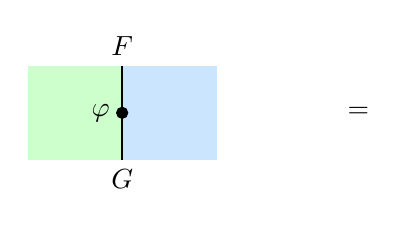
\begin{tikzpicture}[x=0.6cm,y=0.6cm, baseline=(current bounding box.center)]
        % Define colors
        \definecolor{rightcolor}{RGB}{204, 229, 255}
        \definecolor{leftcolor}{RGB}{204,255,204}
    
        % Draw background
        \fill[leftcolor] (0,0) rectangle (2,2);
        \fill[rightcolor] (2,0) rectangle (4,2);
    
        % Draw vertical line and point
        \draw[line width=0.7pt] (2,0) -- (2,2);
        \filldraw [black] (2,1) circle (2pt) node[left=1pt] {$\varphi$};
    
        % Label axes
        \draw (2,0) node[below] {$G$};
        \draw (2,2) node[above] {$F$};
        \draw (7,1) node {$=$};
    \end{tikzpicture}
    \hspace{1cm}
    \begin{tikzcd}[ampersand replacement=\&]
        \mathsf{C} \arrow[r, "F"{name=A, above}, bend left=40] \arrow[r, "G"'{name=B, below}, bend right=40] \&[+30pt] \mathsf{D}
        \arrow[Rightarrow, shorten <=5.5pt, shorten >=5.5pt, from=A.south-|B, to=B, "\varphi"]
    \end{tikzcd}
\end{center}

When we say two string diagrams are equal, we mean that the vertical compositions of natural transformations they represent are equal.

The point(0-cells), strings(1-cells), and 2-cells in a string diagram can be interpreted as follows
\begin{itemize}
    \item 2-cells: categories. 2-cells with different colors represent different categories.
    \item 1-cells: functors. Each 1-cell has exactly two adjacent 2-cells. The left and right adjacent 2-cells are the domain and codomain of the functor respectively. We can think each 1-cell has two end points connected to either a natural transformation or the point at infinity $\infty$. If an end point is connected to $\infty$, then we say that it is a \textbf{free end}. The end point on the top of a string and the end point on the bottom of a string are called the \textbf{top end} and \textbf{bottom end} respectively.
    \item 0-cells: natural transformations. Each 0-cell has exactly two adjacent 1-cells. The top and bottom adjacent 1-cells are the domain and codomain of the natural transformation respectively. 
\end{itemize}

\subsection{Basic Operations}
\subsubsection{Composition of Functors}
If two string $F:\mathsf{C}\to\mathsf{D}$ and $G:\mathsf{D}\to\mathsf{F}$ has the same top ends and bottom ends, then we can glue them together to form a new string $G\circ F$. Depending on whether the top ends and bottom ends are free or not, we can illustrate the following cases


\begin{center}
    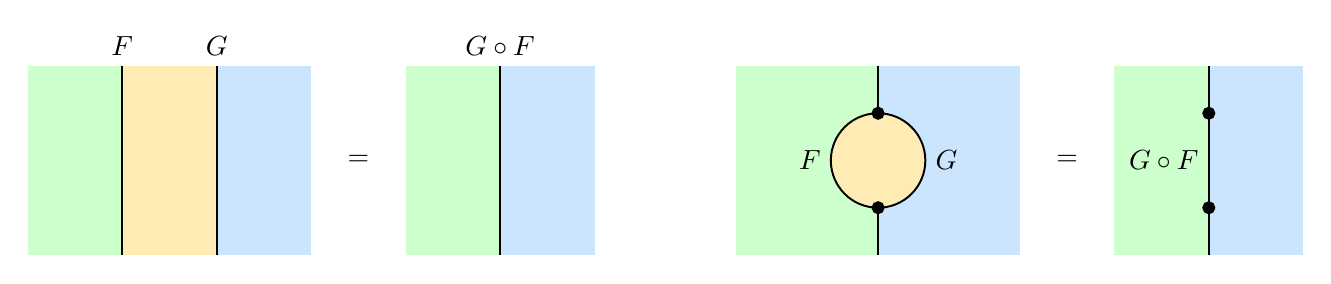
\begin{tikzpicture}[x=0.6cm,y=0.6cm, line width=0.7pt]
            % Define colors
        \definecolor{leftcolor}{RGB}{204,255,204}
        \definecolor{midcolor}{HTML}{FFEBB4} 
        \definecolor{rightcolor}{RGB}{204, 229, 255}
        \begin{scope}
                % Draw background
            \fill[leftcolor] (0,0) rectangle (2,4);
            \fill[midcolor] (2,0) rectangle (4,4);
            \fill[rightcolor] (4,0) rectangle (6,4);
        
            % Draw vertical line and point
            \draw[line width=0.7pt] (2,0) -- (2,4);
            \draw[line width=0.7pt] (4,0) -- (4,4);
    
        
            % Label axes
            \draw (2,4) node[above] {$F$};
            \draw (4,4) node[above] {$G$};
        \end{scope}

        \draw (7,2) node {$=$};

        \begin{scope}[shift={(8,0)}]
            % Draw background
            % Draw background
            \fill[leftcolor] (0,0) rectangle (2,4);
            \fill[rightcolor] (2,0) rectangle (4,4);
        
            % Draw vertical line and point
            \draw[line width=0.7pt] (2,0) -- (2,4);

        
            % Label axes
            \draw (2,4) node[above] {$G\circ F$};
        \end{scope}

        

        \begin{scope}[shift={(16,0)}]
            % Draw background
    
            \fill[leftcolor] (-1,0) rectangle (2,4);
            \fill[rightcolor] (2,0) rectangle (5,4);
            \draw[fill=midcolor, rounded corners=0.6cm, line width=0.7pt] (1,1) rectangle (3, 3);
    
            % Draw vertical line and point
            \draw[line width=0.7pt] (2,0) -- (2,1);
            \draw[line width=0.7pt] (2,3) -- (2,4);
            \filldraw [black] (2,1) circle (2pt);
            \filldraw [black] (2,3) circle (2pt);
        
            % Label axes
            \draw (1,2) node[left] {$F$};
            \draw (3,2) node[right] {$G$};
        \end{scope}
        \draw (22,2) node {$=$};
        \begin{scope}[shift={(23,0)}]
                % Draw background
            % Draw background
            \fill[leftcolor] (0,0) rectangle (2,4);
            \fill[rightcolor] (2,0) rectangle (4,4);
        
            % Draw vertical line and point
            \draw[line width=0.7pt] (2,0) -- (2,4);
            \filldraw [black] (2,1) circle (2pt);
            \filldraw [black] (2,3) circle (2pt);
        
            % Label axes
            \draw (2,2) node[left] {$G\circ F$};
        \end{scope}
    \end{tikzpicture}
\end{center}
\begin{center}
    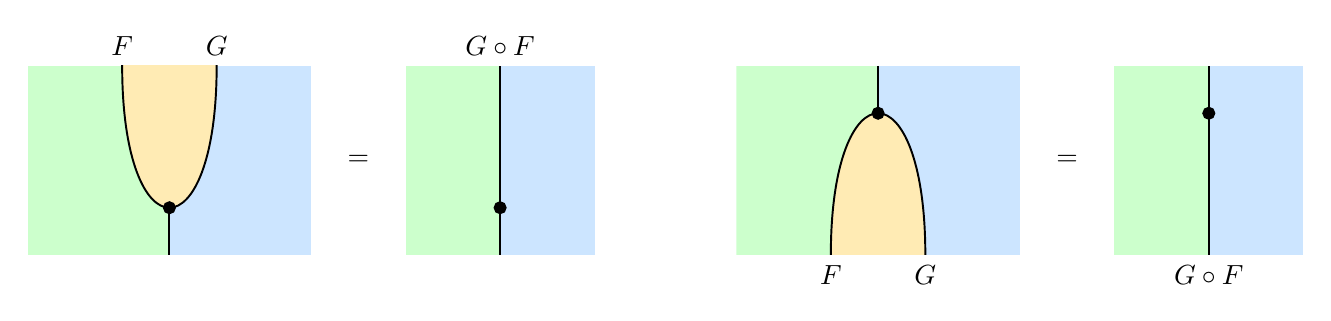
\begin{tikzpicture}[x=0.6cm,y=0.6cm, line width=0.7pt]
        \definecolor{leftcolor}{RGB}{204, 255, 204}
        \definecolor{midcolor}{HTML}{FFEBB4} 
        \definecolor{rightcolor}{RGB}{204, 229, 255}

        \begin{scope}[shift={(0,0)}]
            \begin{scope}
                \clip  (0,0) rectangle (6,4);
                    % Draw background
                \fill[leftcolor] (0,0) rectangle (3,4);
                \fill[rightcolor] (3,0) rectangle (6,4);
                \filldraw[fill=midcolor] (2,5)-- (2,4) .. controls (2,2) and (2.5, 1) .. (3,1).. controls (3.5,1) and (4, 2) .. (4,4)--(4,5)--cycle;
            \end{scope}
        
            % Draw vertical line and point
            \draw[line width=0.7pt] (3,0) -- (3,1);
            \filldraw [black] (3,1) circle (2pt);
            
        
            % Label axes
            \draw (2,4) node[above] {$F$};
            \draw (4,4) node[above] {$G$};
        \end{scope}

        \draw (7,2) node {$=$};

        \begin{scope}[shift={(8,0)}]
            % Draw background
            \fill[leftcolor] (0,0) rectangle (2,4);
            \fill[rightcolor] (2,0) rectangle (4,4);
        
            % Draw vertical line and point
            \draw[line width=0.7pt] (2,0) -- (2,4);
            \filldraw [black] (2,1) circle (2pt);
        
            % Label axes
            \draw (2,4) node[above] {$G\circ F$};
        \end{scope}

            \begin{scope}[shift={(15,0)}]
            \begin{scope}
                \clip  (0,0) rectangle (6,4);
                    % Draw background
                \fill[leftcolor] (0,0) rectangle (3,4);
                \fill[rightcolor] (3,0) rectangle (6,4);
                \filldraw[fill=midcolor] (2,-1)-- (2,0) .. controls (2,2) and (2.5, 3) .. (3,3).. controls (3.5,3) and (4, 2) .. (4,0)--(4,-1)--cycle;
            \end{scope}
        
            % Draw vertical line and point
            \draw[line width=0.7pt] (3,4) -- (3,3);
            \filldraw [black] (3,3) circle (2pt);
            
        
            % Label axes
            \draw (2,0) node[below] {$F$};
            \draw (4,0) node[below] {$G$};
        \end{scope}

        \draw (22,2) node {$=$};

        \begin{scope}[shift={(23,0)}]
            % Draw background
            \fill[leftcolor] (0,0) rectangle (2,4);
            \fill[rightcolor] (2,0) rectangle (4,4);
        
            % Draw vertical line and point
            \draw[line width=0.7pt] (2,0) -- (2,4);
            \filldraw [black] (2,3) circle (2pt);
        
            % Label axes
            \draw (2,0) node[below] {$G\circ F$};
        \end{scope}
    \end{tikzpicture}
\end{center}

\subsubsection{Vertical Composition}
The vertical composition of natural transformations $\varphi:F\Rightarrow H$ and $\psi:G\Rightarrow I$ collapses two adjacent points in a string into one single point and ``eats" the intermediate segment, which is illustrated as follows

\begin{center}
    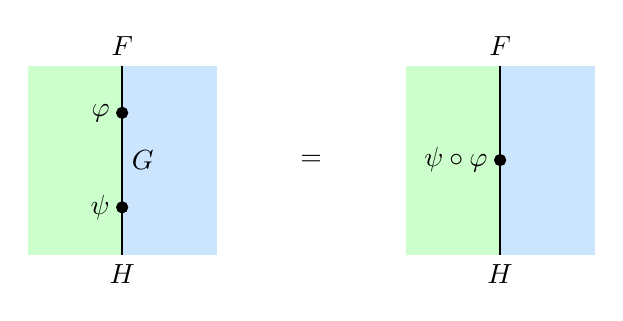
\begin{tikzpicture}[x=0.6cm,y=0.6cm, baseline=(current bounding box.center)]
        % Define colors
        \definecolor{leftcolor}{RGB}{204,255,204}
        \definecolor{rightcolor}{RGB}{204, 229, 255}
        \begin{scope}
            % Draw background
            \fill[leftcolor] (0,-2) rectangle (2,2);
            \fill[rightcolor] (2,-2) rectangle (4,2);
        
        
            % Draw vertical line and point
            \draw[line width=0.7pt] (2,-2) -- (2,2);
            \filldraw [black] (2,1) circle (2pt) node[left=1pt] {$\varphi$};
            \filldraw [black] (2,-1) circle (2pt) node[left=1pt] {$\psi$};
        
            % Label axes
            \draw (2,-2) node[below] {$H$};
            \draw (2,0) node[right] {$G$};
            \draw (2,2) node[above] {$F$};
        \end{scope}

        \draw (6,0) node {$=$};

        \begin{scope}[shift={(8,0)}]
            % Draw background
            \fill[leftcolor] (0,-2) rectangle (2,2);
            \fill[rightcolor] (2,-2) rectangle (4,2);
        
        
            % Draw vertical line and point
            \draw[line width=0.7pt] (2,-2) -- (2,2);
            \filldraw [black] (2,0) circle (2pt) node[left=1pt] {$\psi\circ \varphi$};
    
            % Label axes
            \draw (2,-2) node[below] {$H$};
            \draw (2,2) node[above] {$F$};
        \end{scope}
    \end{tikzpicture}
\end{center}
\subsubsection{Horizontal Composition}
To do horizontal composition for natural transformations $\varphi:F\Rightarrow H$ and $\theta:G\Rightarrow I$ on a horizontal line. First we can stick these two points together, which is illustrated as follows

\begin{center}
    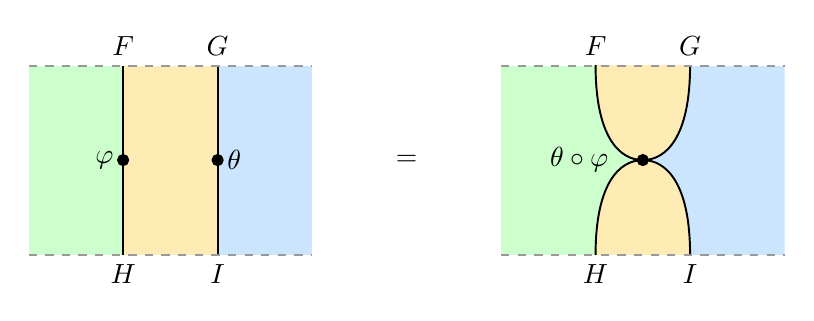
\begin{tikzpicture}[x=0.6cm,y=0.6cm, baseline=(current bounding box.center)]
        \definecolor{leftcolor}{RGB}{204, 255, 204}
        \definecolor{midcolor}{HTML}{FFEBB4} 
        \definecolor{rightcolor}{RGB}{204, 229, 255}

        \begin{scope}
             % Draw background
            \fill[leftcolor] (0,0) rectangle (2,4);
            \fill[midcolor] (2,0) rectangle (4,4);
            \fill[rightcolor] (4,0) rectangle (6,4);
        
            % Draw vertical line and point
            \draw[line width=0.7pt] (2,0) -- (2,4);
            \filldraw [black] (2,2) circle (2pt) node[anchor=east] {$\varphi$};
            \draw[line width=0.7pt] (4,0) -- (4,4);
            \filldraw [black] (4,2) circle (2pt) node[anchor=west] {$\theta$};

            % Draw dashed line
            \draw[dashed, color=black!40, line width=0.7pt] (0,0) -- (6,0);
            \draw[dashed, color=black!40, line width=0.7pt] (0,4) -- (6,4);
        
            % Label axes
            \draw (2,0) node[below] {$H$};
            \draw (2,4) node[above] {$F$};
            \draw (4,0) node[below] {$I$};
            \draw (4,4) node[above] {$G$};
        \end{scope}

        \draw (8,2) node {$=$};

        \begin{scope}[shift={(10,0)}]
             \begin{scope}
                \clip (0,0) rectangle (6,4);
                % Draw background
                \fill[leftcolor] (0,0) rectangle (3,4);
                \fill[rightcolor] (3,0) rectangle (6,4);
                \filldraw[fill=midcolor, line width=0.7pt] (2,5)-- (2,4) .. controls (2, 2.5) and (2.5, 2) .. (3,2).. controls (3.5,2) and (4, 2.5) .. (4,4)--(4,5)--cycle;
                \filldraw[fill=midcolor, line width=0.7pt] (2,-1)-- (2,0) .. controls (2,1.5) and (2.5, 2) .. (3,2).. controls (3.5,2) and (4, 1.5) .. (4,0)--(4,-1)--cycle;
            \end{scope}
        
            % Draw vertical line and point
            \filldraw [black] (3,2) circle (2pt) node[left=9pt] {$\theta\circ\varphi$};

            % Draw dashed line
            \draw[dashed, color=black!40, line width=0.7pt] (0,0) -- (6,0);
            \draw[dashed, color=black!40, line width=0.7pt] (0,4) -- (6,4);

            % Label axes
            \draw (2,0) node[below] {$H$};
            \draw (2,4) node[above] {$F$};
            \draw (4,0) node[below] {$I$};
            \draw (4,4) node[above] {$G$};
        \end{scope}
    \end{tikzpicture}
\end{center}

Then we can composite the functors $F$ and $G$ to get a new functor $G\circ F$. Also we can composite the functors $H$ and $I$ to get a new functor $I\circ H$. By gluing these strings together, we get a new natural transformation $\theta\circ\varphi:G\circ F\Rightarrow I\circ H$. This is illustrated as follows


\begin{center}
    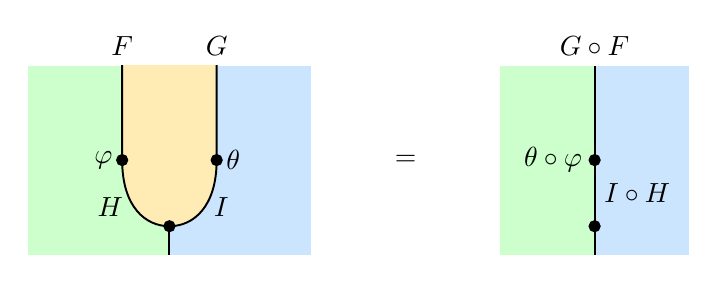
\begin{tikzpicture}[x=0.6cm,y=0.6cm]
        \definecolor{leftcolor}{RGB}{204, 255, 204}
        \definecolor{midcolor}{HTML}{FFEBB4} 
        \definecolor{rightcolor}{RGB}{204, 229, 255}

        \begin{scope}[shift={(0,0)}]
            \begin{scope}
                \clip  (0,0) rectangle (6,4);
                 % Draw background
                \fill[leftcolor] (0,0) rectangle (3,4);
                \fill[rightcolor] (3,0) rectangle (6,4);
                \filldraw[fill=midcolor, line width=0.7pt] (2,5)-- (2,2) .. controls (2,1) and (2.5, 0.6) .. (3,0.6).. controls (3.5,0.6) and (4, 1) .. (4,2)--(4,5)--cycle;
            \end{scope}
        
            % Draw vertical line and point
            \draw[line width=0.7pt] (3,0) -- (3,0.6);
            \filldraw [black] (3,0.6) circle (2pt);
            \filldraw [black] (2,2) circle (2pt) node[anchor=east] {$\varphi$};
            \filldraw [black] (4,2) circle (2pt) node[anchor=west] {$\theta$};

            % Label axes
            \draw (2,4) node[above] {$F$};
            \draw (4,4) node[above] {$G$};
            \draw (1.75,1) node {$H$};
            \draw (4.1,1) node {$I$};
        \end{scope}

        \draw (8,2) node {$=$};

        \begin{scope}[shift={(10,0)}]
            % Draw background
            \fill[leftcolor] (0,0) rectangle (2,4);
            \fill[rightcolor] (2,0) rectangle (4,4);
        
            % Draw vertical line and point
            \draw[line width=0.7pt] (2,0) -- (2,4);
            \filldraw [black] (2,0.6) circle (2pt);
            \filldraw [black] (2,2) circle (2pt) node[left=1pt] {$\theta\circ \varphi$};
            \draw (2, 1.3) node[anchor=west] {$I\circ H$};

            % Label axes
            \draw (2,4) node[above] {$G\circ F$};
        \end{scope}

    \end{tikzpicture}
\end{center}

\subsection{Morphism as Natural Transformation}
If $f:X\to Y$ is a morphism in $\mathsf{C}$, then the following string diagram should be understood as follows
\begin{center}
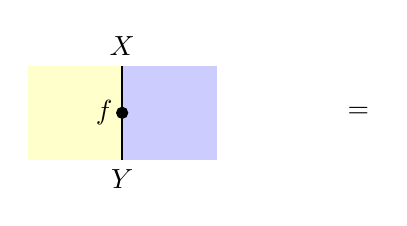
\begin{tikzpicture}[x=0.6cm,y=0.6cm, baseline=(current bounding box.center)]
    % Define colors
    \definecolor{leftcolor}{RGB}{255,255,204} % light yellow
    \definecolor{rightcolor}{RGB}{204,204,255} % light purple

    % Draw background
    \fill[leftcolor] (0,0) rectangle (2,2);
    \fill[rightcolor] (2,0) rectangle (4,2);

    % Draw vertical line and point
    \draw[line width=0.7pt] (2,0) -- (2,2);
    \filldraw [black] (2,1) circle (2pt) node[anchor=east] {$f$};

    % Label axes
    \draw (2,0) node[below] {$Y$};
    \draw (2,2) node[above] {$X$};
    \draw (7,1) node {$=$};
\end{tikzpicture}
\hspace{1cm}
\begin{tikzcd}[ampersand replacement=\&]
    \mathsf{1} \arrow[r, "\diagfunctor X"{name=A, above}, bend left=40] \arrow[r, "\diagfunctor Y"'{name=B, below}, bend right=40] \&[+30pt] \mathsf{C}
    \arrow[Rightarrow, shorten <=5.5pt, shorten >=5.5pt, from=A.south-|B, to=B, "f_{\bullet}"]
\end{tikzcd}
\end{center}
\subsubsection{Naturality}
Suppose $\varphi:F\Rightarrow G$ is a natural transformation between functors $F,G:\mathsf{C}\to \mathsf{D}$. Then the functoriality of $\varphi$ can be described by the following string diagram
\[
    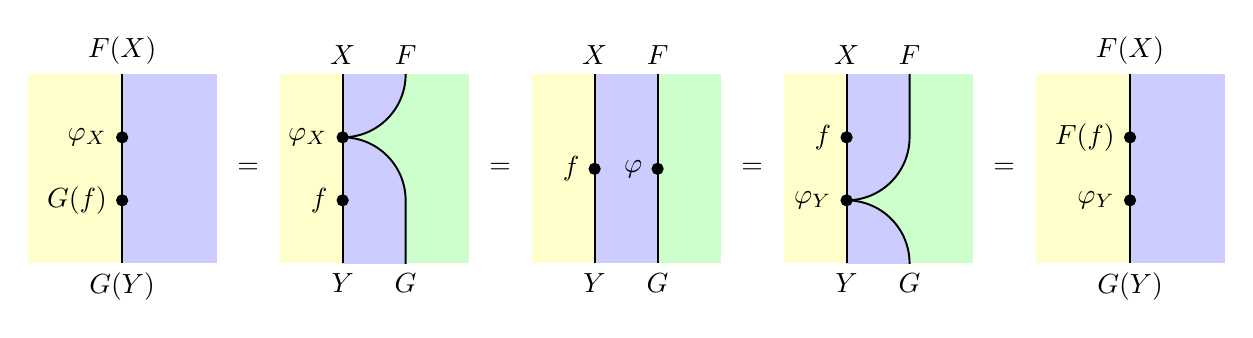
\begin{tikzpicture}[x=0.8cm,y=0.8cm, baseline=(current bounding box.center)]
        % Define colors
        \definecolor{leftcolor}{RGB}{255,255,204} % light yellow
        \definecolor{rightcolor}{RGB}{204,204,255} % light purple
        \begin{scope} [shift={(-3.5,0)}]
        % Draw background
        \fill[leftcolor] (-0.5,0) rectangle (1,3);
        \fill[rightcolor] (1,0) rectangle (2.5,3);
    
        % Draw vertical line and point
        \draw[line width=0.7pt] (1,0) -- (1,3);
        \filldraw [black] (1,1) circle (2pt) node[left=2pt] {$G(f)$};
        \filldraw [black] (1,2) circle (2pt) node[left=2pt] {$\varphi_X$};
        % Label axes
        \draw (1,0) node[below] {$G(Y)$};
        \draw (1,3) node[above] {$F(X)$};
        \draw (3,1.5) node {$=$};
    \end{scope} 
    \begin{scope} 
        % Draw background
        \fill[leftcolor] (0,0) rectangle (1,3);
        \fill[green!20] (1,0) rectangle (3,3);
        \begin{scope} 
            \clip (1,0) rectangle (3, 3); 
            \draw[fill=blue!20, rounded corners=0.8cm, line width=0.7pt] (0,2) rectangle (2, 5);
            \draw[fill=blue!20, rounded corners=0.8cm, line width=0.7pt] (0,2) rectangle (2, -1);
        \end{scope} 
    
        % Draw vertical line and point
        \draw[line width=0.7pt] (1,0) -- (1,3);
        \filldraw [black] (1,1) circle (2pt) node[left=2pt] {$f$};
        \filldraw [black] (1,2) circle (2pt) node[left=2pt] {$\varphi_X$};
        % Label axes
        \draw (1,0) node[below] {$Y$};
        \draw (1,3) node[above] {$X$};
        \draw (2,0) node[below] {$G$};
        \draw (2,3) node[above] {$F$};
        \draw (3.5,1.5) node {$=$};
    \end{scope} 
        
    \begin{scope} [shift={(4,0)}]
        % Define colors
        \definecolor{leftcolor}{RGB}{255,255,204} % light yellow
        \definecolor{rightcolor}{RGB}{204,204,255} % light purple
    
        % Draw background
        \fill[leftcolor] (0,0) rectangle (1,3);
        \fill[blue!20] (1,0) rectangle (2,3);
        \fill[green!20] (2,0) rectangle (3,3);
     
        % Draw vertical line and point
        \draw[line width=0.7pt] (1,0) -- (1,3);
        \draw[line width=0.7pt] (2,0) -- (2,3);
        \filldraw [black] (1,1.5) circle (2pt) node[left=2pt] {$f$};
        \filldraw [black] (2,1.5) circle (2pt) node[left=2pt] {$\varphi$};
        % Label axes
        \draw (1,0) node[below] {$Y$};
        \draw (1,3) node[above] {$X$};
        \draw (2,0) node[below] {$G$};
        \draw (2,3) node[above] {$F$};
        \draw (3.5,1.5) node {$=$};
    \end{scope} 
    
    \begin{scope}[shift={(8,0)}]
        % Define colors
        \definecolor{leftcolor}{RGB}{255,255,204} % light yellow
        \definecolor{rightcolor}{RGB}{204,204,255} % light purple
    
        % Draw background
        \fill[leftcolor] (0,0) rectangle (1,3);
        \fill[green!20] (1,0) rectangle (3,3);
        \begin{scope} 
            \clip (1,0) rectangle (3, 3); 
            \draw[fill=blue!20, rounded corners=0.8cm, line width=0.7pt] (0,1) rectangle (2, 4);
            \draw[fill=blue!20, rounded corners=0.8cm, line width=0.7pt] (0,1) rectangle (2, -2);
            %\fill[color=green!20] (2,0) rectangle (3,3);
            %\filldraw[fill=green!20, rounded corners=1cm] (2, 4) -- (2, 1) -- (1, 1) -- (2, 1) -- (2, -1) -- (4, -1) -- (4, 4) -- cycle;
        \end{scope} 
        % Draw vertical line and point
        \draw[line width=0.7pt] (1,0) -- (1,3);
        \filldraw [black] (1,1) circle (2pt) node[left=2pt] {$\varphi_Y$};
        \filldraw [black] (1,2) circle (2pt) node[left=2pt] {$f$};
        % Label axes
        \draw (1,0) node[below] {$Y$};
        \draw (1,3) node[above] {$X$};
        \draw (2,0) node[below] {$G$};
        \draw (2,3) node[above] {$F$};
        \draw (3.5,1.5) node {$=$};
    \end{scope} 
    
    \begin{scope} [shift={(12.5,0)}]
        % Draw background
        \fill[leftcolor] (-0.5,0) rectangle (1,3);
        \fill[rightcolor] (1,0) rectangle (2.5,3);
    
        % Draw vertical line and point
        \draw[line width=0.7pt] (1,0) -- (1,3);
        \filldraw [black] (1,2) circle (2pt) node[left=2pt] {$F(f)$};
        \filldraw [black] (1,1) circle (2pt) node[left=2pt] {$\varphi_Y$};
        % Label axes
        \draw (1,0) node[below] {$G(Y)$};
        \draw (1,3) node[above] {$F(X)$};
    \end{scope} 
    \end{tikzpicture}
    \]

Note that appending the string diagram 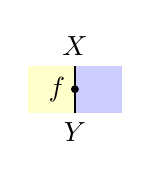
\begin{tikzpicture}[x=0.3cm,y=0.3cm, baseline=(current bounding box.center)]
    % Define colors
    \definecolor{leftcolor}{RGB}{255,255,204} % light yellow
    \definecolor{rightcolor}{RGB}{204,204,255} % light purple

    % Draw background
    \fill[leftcolor] (0,0) rectangle (2,2);
    \fill[rightcolor] (2,0) rectangle (4,2);

    % Draw vertical line and point
    \draw[line width=0.7pt] (2,0) -- (2,2);
    \filldraw [black] (2,1) circle (1.2pt) node[anchor=east] {$f$};

    % Label axes
    \draw (2,0) node[below] {$Y$};
    \draw (2,2) node[above] {$X$};
\end{tikzpicture} to the left of the string diagram of $\varphi$ is equivalent to evaluating $\varphi$ at $f:X\to Y$.

\subsubsection{Elements of Sets}
Let $X$ be a set and $x\in X$ be an element of $X$. Then we represents $x$ as a morphism $x:\{*\}\to X$ in $\mathsf{Set}$, which is illustrated as follows
\begin{center}
    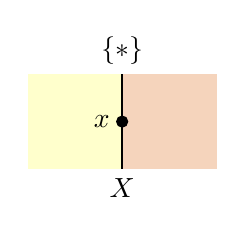
\begin{tikzpicture}[x=0.6cm,y=0.6cm, baseline=(current bounding box.center)]
        % Define colors
        \definecolor{leftcolor}{RGB}{255,255,204} % light yellow
        \definecolor{rightcolor}{HTML}{F5D4BC} % red
    
        % Draw background
        \fill[leftcolor] (0,0) rectangle (2,2);
        \fill[rightcolor] (2,0) rectangle (4,2);
    
        % Draw vertical line and point
        \draw[line width=0.7pt] (2,0) -- (2,2);
        \filldraw [black] (2,1) circle (2pt) node[left=1pt] {$x$};
    
        % Label axes
        \draw (2,0) node[below] {$X$};
        \draw (2,2) node[above] {$\{*\}$};
    \end{tikzpicture}
\end{center}
\subsubsection{Function as Element or Morphism}
If we have a function $f:X\to Y$, then we can represent $f$ as morphism $f:X\to Y$ in $\mathsf{Set}$, which is illustrated as follows
\[
    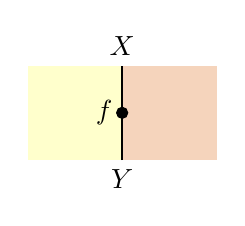
\begin{tikzpicture}[x=0.6cm,y=0.6cm, baseline=(current bounding box.center)]
        % Define colors
        \definecolor{leftcolor}{RGB}{255,255,204} % light yellow
        \definecolor{rightcolor}{HTML}{F5D4BC}  % red
    
        % Draw background
        \fill[leftcolor] (0,0) rectangle (2,2);
        \fill[rightcolor] (2,0) rectangle (4,2);
    
        % Draw vertical line and point
        \draw[line width=0.7pt] (2,0) -- (2,2);
        \filldraw [black] (2,1) circle (2pt) node[anchor=east] {$f$};
    
        % Label axes
        \draw (2,0) node[below] {$Y$};
        \draw (2,2) node[above] {$X$};
    \end{tikzpicture}
\]
And we can also represent $f$ as an element $f\in \mathrm{Hom}_{\mathsf{Set}}(X,Y)$, which is illustrated as follows
\[
    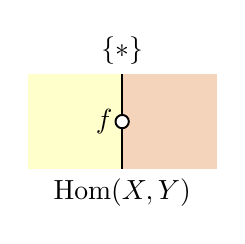
\begin{tikzpicture}[
        x=0.6cm,
        y=0.6cm,
        mydot/.style={
            circle,
            fill=white,
            draw,
            outer sep=0pt,
            inner sep=1.7pt,
            line width=0.7pt
          }]
        % Define colors
        \definecolor{leftcolor}{RGB}{255,255,204} % light yellow
        \definecolor{rightcolor}{HTML}{F5D4BC}  % red
    
        % Draw background
        \fill[leftcolor] (0,0) rectangle (2,2);
        \fill[rightcolor] (2,0) rectangle (4,2);
    
        % Draw vertical line and point
        \draw[line width=0.7pt] (2,0) -- (2,2);
        \draw (2,1) node[mydot] {};
        \draw (2,1) node[left] {$f$};
    
        % Label axes
        \draw (2,0) node[below] {$\mathrm{Hom}(X,Y)$};
        \draw (2,2) node[above] {$\{*\}$};
    \end{tikzpicture}
\]
Then we have the following equalities for Hom functor $\llbracket X , -\rrbracket:\mathsf{C}\to \mathsf{Set}$
\[
 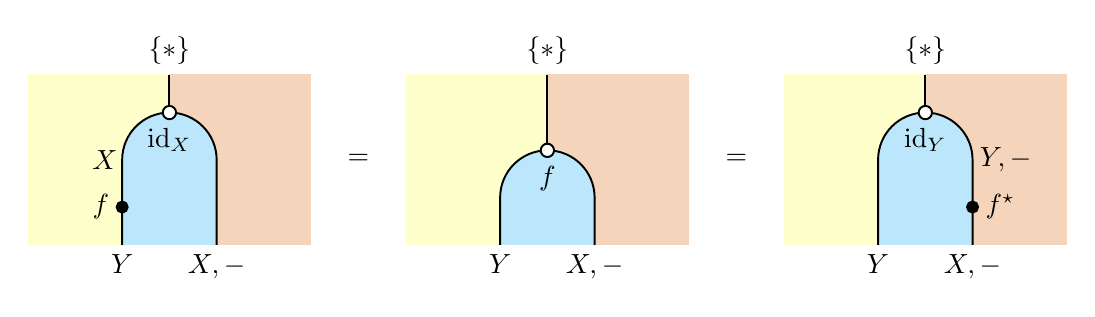
\begin{tikzpicture}[x=0.6cm,y=0.6cm,line width=0.7pt,hollow/.style={
            circle,
            fill=white,
            draw,
            outer sep=0pt,
            inner sep=1.7pt,
            line width=0.7pt
          }]
    \definecolor{leftcolor}{RGB}{255,255,204}
    \definecolor{midcolor}{HTML}{BBE6FB}
    \definecolor{rightcolor}{HTML}{F5D4BC}

    \node at (4, 1.8) {$=$};
    \node at (12, 1.8) {$=$};
    
    \begin{scope}
        \begin{scope} 
            \clip (-3,0) rectangle (3,3.6);     
            \fill[fill=leftcolor] (-3,0) rectangle (0, 4);  
            \fill[fill=rightcolor] (0,0) rectangle (3, 4);  
            \draw[fill=midcolor, rounded corners=0.6cm, line width=0.7pt] (-1, -2) rectangle (1, 2.8);
        \end{scope}
        \draw (0, 3.6) -- (0,2.8);
        \filldraw [black] (-1,0.8) circle (2pt) node[left=1pt] {$f$};
        \node[below] at (-1, 0) {$Y$};
        \node[left=-2pt] at (-1, 1.8) {$X$};
        \node[below] at (1, 0) {$\llbracket X , -\rrbracket$};
        \node[hollow] at (0, 2.8) {};
        \node[below=2pt] at (0, 2.8) {$\mathrm{id}_X$}; 
        \node[above] at (0, 3.6) {$\{*\}$};
    \end{scope}
    
    \begin{scope}[shift={(8,0)}]
        \begin{scope} 
            \clip (-3,0) rectangle (3,3.6);     
            \fill[fill=leftcolor] (-3,0) rectangle (0, 4);  
            \fill[fill=rightcolor] (0,0) rectangle (3, 4);  
            \draw[fill=midcolor, rounded corners=0.6cm, line width=0.7pt] (-1, -2) rectangle (1, 2);
        \end{scope}
        \draw (0, 3.6) -- (0,2);
        \node[below] at (-1, 0) {$Y$};
        \node[below] at (1, 0) {$\llbracket X , -\rrbracket$};
        \node[hollow] at (0, 2) {};
        \node[below=2pt] at (0, 2) {$f$}; 
        \node[above] at (0, 3.6) {$\{*\}$};
    \end{scope}
    
     \begin{scope}[shift={(16,0)}]
        \begin{scope} 
            \clip (-3,0) rectangle (3, 3.6);     
            \fill[fill=leftcolor] (-3,0) rectangle (0, 4);  
            \fill[fill=rightcolor] (0,0) rectangle (3, 4);  
            \draw[fill=midcolor, rounded corners=0.6cm, line width=0.7pt] (-1, -2) rectangle (1, 2.8);
        \end{scope}
        \draw (0, 3.6) -- (0,2.8);
        \filldraw [black] (1,0.8) circle (2pt) node[right=1pt] {$f^\star$};
        \node[below] at (-1, 0) {$Y$};
        \node[right=-1pt] at (1, 1.8) {$\llbracket Y , -\rrbracket$};
        \node[below] at (1, 0) {$\llbracket X , -\rrbracket$};
        \node[hollow] at (0, 2.8) {};
        \node[below=2pt] at (0, 2.8) {$\mathrm{id}_Y$}; 
        \node[above] at (0, 3.6) {$\{*\}$};
    \end{scope}
    
    \end{tikzpicture}
\]
Generally, given $X\xrightarrow{f}Y_1\xrightarrow{g}Y_2$ in $\mathsf{Set}$, we have the following equalities
\[
 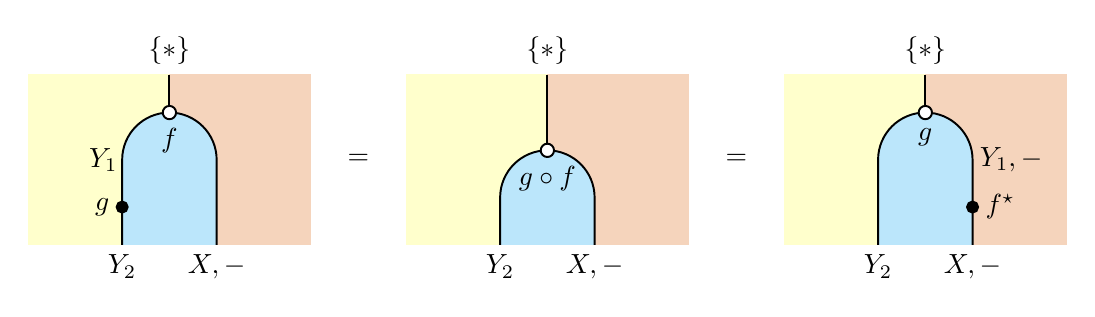
\begin{tikzpicture}[x=0.6cm,y=0.6cm,line width=0.7pt,hollow/.style={
            circle,
            fill=white,
            draw,
            outer sep=0pt,
            inner sep=1.7pt,
            line width=0.7pt
          }]
    \definecolor{leftcolor}{RGB}{255,255,204}
    \definecolor{midcolor}{HTML}{BBE6FB}
    \definecolor{rightcolor}{HTML}{F5D4BC}

    \node at (4, 1.8) {$=$};
    \node at (12, 1.8) {$=$};
    
    \begin{scope}
        \begin{scope} 
            \clip (-3,0) rectangle (3,3.6);     
            \fill[fill=leftcolor] (-3,0) rectangle (0, 4);  
            \fill[fill=rightcolor] (0,0) rectangle (3, 4);  
            \draw[fill=midcolor, rounded corners=0.6cm, line width=0.7pt] (-1, -2) rectangle (1, 2.8);
        \end{scope}
        \draw (0, 3.6) -- (0,2.8);
        \filldraw [black] (-1,0.8) circle (2pt) node[left=1pt] {$g$};
        \node[below] at (-1, 0) {$Y_2$};
        \node[left=-2pt] at (-1, 1.8) {$Y_1$};
        \node[below] at (1, 0) {$\llbracket X , -\rrbracket$};
        \node[hollow] at (0, 2.8) {};
        \node[below=2pt] at (0, 2.8) {$f$}; 
        \node[above] at (0, 3.6) {$\{*\}$};
    \end{scope}
    
    \begin{scope}[shift={(8,0)}]
        \begin{scope} 
            \clip (-3,0) rectangle (3,3.6);     
            \fill[fill=leftcolor] (-3,0) rectangle (0, 4);  
            \fill[fill=rightcolor] (0,0) rectangle (3, 4);  
            \draw[fill=midcolor, rounded corners=0.6cm, line width=0.7pt] (-1, -2) rectangle (1, 2);
        \end{scope}
        \draw (0, 3.6) -- (0,2);
        \node[below] at (-1, 0) {$Y_2$};
        \node[below] at (1, 0) {$\llbracket X , -\rrbracket$};
        \node[hollow] at (0, 2) {};
        \node[below=2pt] at (0, 2) {$g\circ f$}; 
        \node[above] at (0, 3.6) {$\{*\}$};
    \end{scope}
    
     \begin{scope}[shift={(16,0)}]
        \begin{scope} 
            \clip (-3,0) rectangle (3, 3.6);     
            \fill[fill=leftcolor] (-3,0) rectangle (0, 4);  
            \fill[fill=rightcolor] (0,0) rectangle (3, 4);  
            \draw[fill=midcolor, rounded corners=0.6cm, line width=0.7pt] (-1, -2) rectangle (1, 2.8);
        \end{scope}
        \draw (0, 3.6) -- (0,2.8);
        \filldraw [black] (1,0.8) circle (2pt) node[right=1pt] {$f^\star$};
        \node[below] at (-1, 0) {$Y_2$};
        \node[right=-1pt] at (1, 1.8) {$\llbracket Y_1 , -\rrbracket$};
        \node[below] at (1, 0) {$\llbracket X , -\rrbracket$};
        \node[hollow] at (0, 2.8) {};
        \node[below=2pt] at (0, 2.8) {$g$}; 
        \node[above] at (0, 3.6) {$\{*\}$};
    \end{scope}
    
    \end{tikzpicture}
\]
\section{Representable Functor}
\dfn{Presheaf}{
    Let $\mathsf{C}$ be a category. A \textbf{presheaf} on $\mathsf{C}$ is a functor $F:\mathsf{C}^{\mathrm{op}}\to \mathsf{Set}$.
}

\dfn[yoneda_embedding_functor]{Yoneda Embedding Functor}{
    Let $\mathsf{C}$ be a category. The \textbf{Yoneda embedding functor} is the functor $Y_\mathsf{C}:\mathsf{C}\to \left[\mathsf{C}^{\mathrm{op}},\mathsf{Set}\right]$ defined as follows
    \[
    \begin{tikzcd}[ampersand replacement=\&]
    \mathsf{C} % column 1
    \&[-25pt]  % column 2
    \&[+30pt]  % column 3
    \&[-30pt] \left[\mathsf{C}^{\mathrm{op}},\mathsf{Set}\right]    % column 4
    \&[+25pt]  % column 5
    \&[-25pt]  % column 6 
    \&         % column 7
    \\[-15pt]
    Y_1 \arrow[dd, "g"{name=L, left}] \&\&  \& \mathrm{Hom}_{\mathsf{C}}\left(-,Y_1\right) \arrow[dd, Rightarrow, "g_\star"{name=R}] \& \mathrm{Hom}_{\mathsf{C}}(X_1,Y_1) \arrow[dd, "{g_*}"'] \arrow[rr, "{f^*}"] \& \& \mathrm{Hom}_{\mathsf{C}}(X_2,Y_1) \arrow[dd, "g_*"] \\[-5pt]
    \& \phantom{.}\arrow[r, "Y_\mathsf{C}", squigarrow]\&\phantom{.} \&\phantom{.} \&\phantom{.}\&\\[-5pt]
    Y_2 \& \& \& \mathrm{Hom}_{\mathsf{C}}\left(-,Y_2\right)\& \mathrm{Hom}_{\mathsf{C}}(X_1,Y_2) \arrow[rr, "{f^*}"'] \& \& \mathrm{Hom}_{\mathsf{C}}(X_2,Y_2) 
    \arrow[from=4-5, to=2-5, dash, start anchor={[xshift=-8ex,yshift=-3ex]}, end anchor={[xshift=-8ex,yshift=3ex]},decorate,decoration={brace,amplitude=10pt,raise=4pt}] 
    \arrow[from=3-4, to=3-5, dashed, start anchor={[xshift=9pt, yshift=-2pt]}, end anchor={[xshift=-11ex, yshift=-2pt]},decorate] 
    \end{tikzcd}
    \]
    where the natural transformation $g_\star$ is defined pointwise as follows: $\left(g_\star\right)_X=g_*$ for any $X\in \mathrm{Ob}(\mathsf{C}^{\mathrm{op}})$.\\
    The contravariant version is $Y_{\mathsf{C}^{\mathrm{op}}}:\mathsf{C}^{\mathrm{op}}\to \left[\mathsf{C},\mathsf{Set}\right]$, which is defined as follows
    \[
    \begin{tikzcd}[ampersand replacement=\&]
    \mathsf{C}^{\mathrm{op}} % column 1
    \&[-25pt]  % column 2
    \&[+30pt]  % column 3
    \&[-30pt] \left[\mathsf{C},\mathsf{Set}\right]    % column 4
    \&[+25pt]  % column 5
    \&[-25pt]  % column 6 
    \&         % column 7
    \\[-15pt]
    X_1 \arrow[dd, "f"{name=L, left}] \&\&  \& \mathrm{Hom}_{\mathsf{C}}\left(X_1,-\right) \arrow[dd, Rightarrow, "f^\star"{name=R}] \& \mathrm{Hom}_{\mathsf{C}}(X_1,Y_1) \arrow[dd, "{f^*}"'] \arrow[rr, "{g_*}"] \& \& \mathrm{Hom}_{\mathsf{C}}(X_1,Y_2) \arrow[dd, "f^*"] \\[-5pt]
    \& \phantom{.}\arrow[r, "Y_{\mathsf{C}^{\mathrm{op}}}", squigarrow]\&\phantom{.} \&\phantom{.} \&\phantom{.}\&\\[-5pt]
    X_2 \& \& \& \mathrm{Hom}_{\mathsf{C}}\left(X_2,-\right)\& \mathrm{Hom}_{\mathsf{C}}(X_2,Y_1) \arrow[rr, "{g_*}"'] \& \& \mathrm{Hom}_{\mathsf{C}}(X_2,Y_2) 
    \arrow[from=4-5, to=2-5, dash, start anchor={[xshift=-8ex,yshift=-3ex]}, end anchor={[xshift=-8ex,yshift=3ex]},decorate,decoration={brace,amplitude=10pt,raise=4pt}] 
    \arrow[from=3-4, to=3-5, dashed, start anchor={[xshift=9pt, yshift=-2pt]}, end anchor={[xshift=-11ex, yshift=-2pt]},decorate] 
    \end{tikzcd}
    \]
    Here we use the fact $\mathrm{Hom}_{\mathsf{C}^{\mathrm{op}}}\left(-,X\right)=\mathrm{Hom}_{\mathsf{C}}\left(X,-\right)$.
    
}
\thm[yoneda_lemma]{Yoneda Lemma}{
    Let $\mathsf{C}$ be a locally small category. For any functor $F:\mathsf{C}^{\mathrm{op}}\to \mathsf{Set}$ and any $A\in \mathrm{Ob}(\mathsf{C})$, there is a natural bijection
    \begin{align*}
        q_{A,F}:\operatorname{Hom}_{\mathsf{Psh}(\mathsf{C})}\left(\operatorname{Hom}_{\mathsf{C}}\left(-,A\right), F\right) & \overset{\sim}{\longrightarrow} F(A) \\
        {  \left[ \begin{tikzcd}[ampersand replacement=\&]
            \mathsf{C}^{\mathrm{op}} \arrow[r, "\operatorname{Hom}_{\mathsf{C}}\left(-{,}A\right)"{name=A, above}, bend left] \arrow[r, "F"'{name=B, below}, bend right] \&[+30pt] \mathsf{Set}
            \arrow[Rightarrow, shorten <=5.5pt, shorten >=5.5pt, from=A.south-|B, to=B, "\phi"]
        \end{tikzcd}\right] } & \longmapsto \phi_A\left(\operatorname{id}_A\right)
    \end{align*}
    The naturality of $q_{A,F}$ means that 
    \[
        \begin{tikzcd}[ampersand replacement=\&]
            \mathsf{C}^{\mathrm{op}}\times \left[\mathsf{C}^{\mathrm{op}},\mathsf{Set}\right]\&[-34pt]\&[+62pt]\&[-25pt] \mathsf{Set}\&[-25pt]\&[-25pt] \\ [-15pt] 
            (A_1,F_1)  \arrow[dd, "\left(g{,} \eta\right)"{name=L, left}] 
            \&[-25pt] \& [+10pt] 
            \& [-30pt]\operatorname{Hom}_{\mathsf{Psh}(\mathsf{C})}(\mathrm{Hom}_{\mathsf{C}}(-,A_1),F_1)\arrow[dd, ""{name=R}] \& \ni \& \phi \arrow[dd,mapsto]\\ [-8pt] 
            \&  \phantom{.}\arrow[r, "\operatorname{Hom}_{\mathsf{Psh}(\mathsf{C})}\left(Y_\mathsf{C}(-){,}-\right)", squigarrow]\&\phantom{.}  \&   \\[-8pt] 
            (A_2,F_2)  \& \& \& \operatorname{Hom}_{\mathsf{Psh}(\mathsf{C})}(\mathrm{Hom}_{\mathsf{C}}(-,A_2),F_2)\& \ni \& \eta\circ \phi\circ g_\star
        \end{tikzcd}
    \]
    is a functor isomorphic to the \hyperref[th:evaluation_functor]{evaluation functor}
    \begin{align*}
        \mathrm{ev}:\mathsf{C}^{\mathrm{op}}\times \left[\mathsf{C}^{\mathrm{op}},\mathsf{Set}\right]&\longrightarrow \mathsf{Set}\\
        \left(A,F\right)&\longmapsto F(A)
    \end{align*}
    \textbf{Covariant version}\\
    For any functor $F:\mathsf{C}\to \mathsf{Set}$ and any $A\in \mathrm{Ob}(\mathsf{C})$, there is a natural bijection
    \begin{align*}
        \operatorname{Hom}_{\left[\mathsf{C},\mathsf{Set}\right]}\left(\operatorname{Hom}_{\mathsf{C}}\left(A,-\right), F\right) & \overset{\sim}{\longrightarrow} F(A) \\
        {  \left[ \begin{tikzcd}[ampersand replacement=\&]
            \mathsf{C} \arrow[r, "\operatorname{Hom}_{\mathsf{C}}\left(A{,}-\right)"{name=A, above}, bend left] \arrow[r, "F"'{name=B, below}, bend right] \&[+30pt] \mathsf{Set}
            \arrow[Rightarrow, shorten <=5.5pt, shorten >=5.5pt, from=A.south-|B, to=B, "\phi"]
        \end{tikzcd}\right] } & \longmapsto \phi_A\left(\operatorname{id}_A\right)
    \end{align*}
}
\pf{
    We break the proof into following steps.
\begin{itemize}[leftmargin=*]
    \item \textbf{$\phi$ is determined by $\phi_A\left(\operatorname{id}_A\right)$}.\\
    Suppose $\phi:\mathrm{Hom}_{\mathsf{C}}\left(-,A\right)\Rightarrow F$ is a natural transformation. Given any morphism $f:X\to A$ in $\mathsf{C}$, the naturality of $\phi$ gives the following commutative diagram
    \[
		\begin{tikzcd}[ampersand replacement=\&, row sep = 3.5em]
			\mathrm{id}_A\arrow[d, mapsto]\&[-25pt]\in\&[-25pt]\mathrm{Hom}_{\mathsf{C}}(A,A) \arrow[d, "{\phi_A}"']  \arrow[rr, "{f^*}"] \&[-20pt] \& {\mathrm{Hom}_{\mathsf{C}}(X,A)} \arrow[d, "\phi_X"]\&[-25pt]\ni\&[-25pt]f \arrow[d, mapsto]\\
			\phi_A(\mathrm{id}_A)\&\in\&{F(A)}\arrow[rr, "{F(f)}"'] \&  \& {F(X)}  \&\ni\& \phi_X(f)     
		\end{tikzcd}
	\]
    Thus we see $\phi$ is determined by $\phi_A(\mathrm{id}_A)$ as follows
    \[
        \phi_X(f)=F(f)(\phi_A(\mathrm{id}_A)),\quad\forall X\in \mathrm{Ob}(\mathsf{C}),\forall f\in \mathrm{Hom}_{\mathsf{C}}(X,A).
    \]
    This implies that the injectivity of $q_{A,F}$.
    \item \textbf{Construct the inverse of $q_{A,F}$}.\\
    Define 
    \begin{align*}
        r_{A,F}:  F(A)&\longrightarrow\operatorname{Hom}_{\mathsf{Psh}(\mathsf{C})}\left(\operatorname{Hom}_{\mathsf{C}}\left(-,A\right), F\right) \\
         u & \longmapsto \phi^u:\left[\begin{aligned}\phi_X^u: \mathrm{Hom}_{\mathsf{C}}(X,A)&\longrightarrow F(X)\\
             f&\longmapsto F(f)(u)\end{aligned}  \right]
    \end{align*}
    To ensure $r_{A,F}$ is well-defined, we need to check that $r_{A,F}(u)=\phi^u$ is always a natural transformation. In fact, given any morphism $h:X_1\to X_2$ in $\mathsf{C}$, it is easy to check the following diagram commutes
    \[
        \begin{tikzcd}[ampersand replacement=\&, row sep = 3.5em]
                g\arrow[mapsto]{d}\&[-25pt]\in\&[-25pt]\mathrm{Hom}_{\mathsf{C}}(X_2,A) \arrow[d, "{\phi_{X_2}^u}"']  \arrow[rr, "{h^*}"] \&[-20pt] \& {\mathrm{Hom}_{\mathsf{C}}(X_1,A)} \arrow[d, "\phi_{X_1}^u"]\&[-25pt]\ni\&[-25pt]g\circ h \arrow[mapsto]{d}\\
                F(g)(u)\&\in\&{F(X_2)}\arrow[rr, "{F(h)}"'] \&  \& {F(X_1)}  \&\ni\& F(g\circ h)(u)  
            \end{tikzcd}
    \]
    because the functoriality of $F$ gives the identity $F(g\circ h)=F(h)\circ F(g)$.

    For any $u\in F(A)$, we have
    \begin{align*}
        \left(q_{A,F}\circ r_{A,F}\right)(u)
        &=q_{A,F}(\phi^u)\\
        &=\phi^u_A(\mathrm{id}_A)\\
        &=F(\mathrm{id}_A)(u)\\
        &=\mathrm{id}_{F(A)}(u)\\
        &=u,
    \end{align*}
    which implies that $q_{A,F}$ is surjective. Therefore, $q_{A,F}$ is a bijection and $r_{A,F}$ is the inverse of $q_{A,F}$.

    We can also manually check that $\left(r_{A,F}\circ q_{A,F}\right)(\phi)=\phi$ for any natural transformation $\phi:\mathrm{Hom}_{\mathsf{C}}\left(-,A\right)\Rightarrow F$, by evaluating the natural transformations at $\mathrm{id}_A$,
    \begin{align*}
        \left(\left(r_{A,F}\circ q_{A,F}\right)(\phi)\right)_A(\mathrm{id}_A)&=(r_{A,F}(\phi_A(\mathrm{id}_A)))_A(\mathrm{id}_A)\\
        &=F(\mathrm{id}_A)(\phi_A(\mathrm{id}_A))\\
        &=\mathrm{id}_{F(A)}(\phi_A(\mathrm{id}_A))\\
        &=\phi_A(\mathrm{id}_A).
    \end{align*}
    \item \textbf{$q_{A,F}$ is natural in $A$ and $F$}.\\
    $\operatorname{Hom}_{\mathsf{Psh}(\mathsf{C})}\left(Y_\mathsf{C}(-){,}-\right)$ is a functor obtained by the composition 
    \[
        \mathsf{C}^{\mathrm{op}}\times \left[\mathsf{C}^{\mathrm{op}},\mathsf{Set}\right]\xrightarrow{\left(Y^{\mathrm{op}}_{\mathsf{C}},\mathrm{id}\right)}\left[\mathsf{C}^{\mathrm{op}},\mathsf{Set}\right]^{\mathrm{op}}\times \left[\mathsf{C}^{\mathrm{op}},\mathsf{Set}\right]\xrightarrow{\mathrm{Hom}_{\mathsf{Psh}(\mathsf{C})}\left(-,-\right)}\mathsf{Set}
    \]
    Given any $g:A_2\to A_1$ and $\eta:F_1\to F_2$, we should check the following diagram commutes
    \[
        \begin{tikzcd}[row sep=3.5em, column sep=2.5em, ampersand replacement=\&]
        {\operatorname{Hom}_{\mathsf{Psh}(\mathsf{C})}(Y_\mathsf{C}(A_1),F_1)} \arrow[d, "{q_{A_1,F_1}}"'] \arrow[rr, "\left(g_\star\right)^*\circ \eta_*"] \&  \& {\operatorname{Hom}_{\mathsf{Psh}(\mathsf{C})}(Y_\mathsf{C}(A_2),F_2)} \arrow[d, "q_{A_2,F_2}"] \\
        {F_1(A_1)} \arrow[rr, "F_2(g)\circ \eta_{A_1}"']      \&  \& {F_2(A_2)}               
    \end{tikzcd}
    \]
    It suffices to check that the following diagram commutes
    \[
    \begin{tikzcd}[ampersand replacement=\&, row sep = 3.5em]
        \operatorname{Hom}(Y_\mathsf{C}(A_1),F_1) \arrow[rr,"\left(g_\star\right)^*"] \arrow[dr,swap,"\eta_*"] \arrow[dd,swap,"q_{A_1,F_1}"] \&\&
        \operatorname{Hom}(Y_\mathsf{C}(A_2),F_1) \arrow[dd,swap,"q_{A_2,F_1}" near start] \arrow[dr,"\eta_*"] \\
        \& \operatorname{Hom}(Y_\mathsf{C}(A_1),F_2) \arrow[rr,crossing over,"\left(g_\star\right)^*" near start] \&\&
        \operatorname{Hom}(Y_\mathsf{C}(A_2),F_2) \arrow[dd,"q_{A_2,F_2}"] \\
        F_1(A_1) \arrow[rr,"F_1(g)" near end] \arrow[dr,swap,"\eta_{A_1}"] \&\& F_1(A_2) \arrow[dr,swap,"\eta_{A_2}"] \\
        \& F_2(A_1) \arrow[rr,"F_2(g)"] \arrow[uu,<-,crossing over,"q_{A_1,F_2}" near end]\&\& F_2(A_2)
        \end{tikzcd}
    \]
\end{itemize}
    To check the commutativity of the left square
    \[
        \begin{tikzcd}[row sep=3.5em, column sep=2.5em, ampersand replacement=\&]
        {\operatorname{Hom}_{\mathsf{Psh}(\mathsf{C})}(Y_\mathsf{C}(A_1),F_1)} \arrow[d, "{q_{A_1,F_1}}"'] \arrow[rr, "\eta_*"] \&  \& {\operatorname{Hom}_{\mathsf{Psh}(\mathsf{C})}(Y_\mathsf{C}(A_1),F_2)} \arrow[d, "q_{A_1,F_2}"] \\
        {F_1(A_1)} \arrow[rr, "\eta_{A_1}"']      \&  \& {F_2(A_1)}               
    \end{tikzcd}
    \]
    we can verify that for any $\phi\in \operatorname{Hom}_{\mathsf{Psh}(\mathsf{C})}\left(Y_\mathsf{C}(A_1),F_1\right)$, 
    \begin{align*}
        q_{A_1,F_2}\circ \eta_*\left(\phi\right)&=q_{A_1,F_2}\left(\eta\circ \phi\right)\\
        &=\left(\eta\circ \phi\right)_{A_1}\left(\mathrm{id}_{A_1}\right)\\
        &=\eta_{A_1}(\phi_{A_1}(\mathrm{id}_{A_1}))\\
        &=\eta_{A_1}\circ q_{A_1,F_1}(\phi).
    \end{align*}
    To check the commutativity of the front square
    \[
        \begin{tikzcd}[row sep=3.5em, column sep=2.5em, ampersand replacement=\&]
        {\operatorname{Hom}_{\mathsf{Psh}(\mathsf{C})}(Y_\mathsf{C}(A_1),F_2)} \arrow[d, "{q_{A_1,F_2}}"'] \arrow[rr, "\left(g_\star\right)^*"] \&  \& {\operatorname{Hom}_{\mathsf{Psh}(\mathsf{C})}(Y_\mathsf{C}(A_2),F_2)} \arrow[d, "q_{A_2,F_2}"] \\
        {F_2(A_1)} \arrow[rr, "F_2(g)"']      \&  \& {F_2(A_2)}               
    \end{tikzcd}
    \]
    we can verify that for any $\psi\in \operatorname{Hom}_{\mathsf{Psh}(\mathsf{C})}\left(Y_\mathsf{C}(A_1),F_2\right)$, we have
    \begin{align*}
        q_{A_2,F_2}\circ \left(g_\star\right)^*(\psi)&=q_{A_2,F_2}\left(\psi\circ g_\star\right)\\
        &=\left(\psi\circ g_\star\right)_{A_2}\left(\mathrm{id}_{A_2}\right)\\
        &=\psi_{A_2}\circ g_*\left(\mathrm{id}_{A_2}\right)\\
        &=\psi_{A_2}(g)\\
        &=F_2(g)(\psi_{A_1}(\mathrm{id}_{A_1}))\\
        &=F_2(g)\circ q_{A_1,F_2}(\psi).
    \end{align*}
}
\noindent For the covariant version, the following string diagram shows $\phi$ is determined by $\phi_A\left(\operatorname{id}_A\right)$
\[
        \phi_X(f)=F(f)(\phi_A(\mathrm{id}_A)),\quad\forall X\in \mathrm{Ob}(\mathsf{C}),\forall f\in \mathrm{Hom}_{\mathsf{C}}(A,X).
\]
\[
    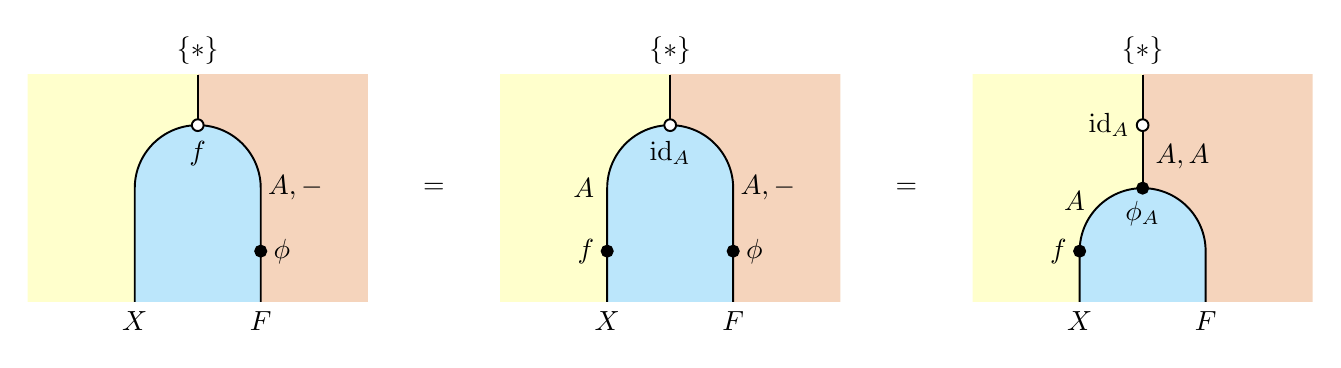
\begin{tikzpicture}[x=0.8cm,y=0.8cm, line width=0.7pt, hollow/.style={
            circle,
            fill=white,
            draw,
            outer sep=0pt,
            inner sep=1.5pt,
            line width=0.7pt
          }]
        % Define colors
         \definecolor{leftcolor}{RGB}{255,255,204}
    \definecolor{midcolor}{HTML}{BBE6FB}
    \definecolor{rightcolor}{HTML}{F5D4BC}

    \node at (-3.75, 1.8) {$=$};
    \node at (3.75, 1.8) {$=$};

    \begin{scope}[shift={(-7.5,0)}]
        \begin{scope} 
            \clip (-2.7,0) rectangle (2.7, 3.6);     
            \fill[fill=leftcolor] (-3,0) rectangle (0, 4);  
            \fill[fill=rightcolor] (0,0) rectangle (3, 4);  
            \draw[fill=midcolor, rounded corners=0.8cm, line width=0.7pt] (-1, -2) rectangle (1, 2.8);
        \end{scope}
        \draw (0, 3.6) -- (0,2.8);
        \filldraw [black] (1,0.8) circle (2pt) node[right=1pt] {$\phi$};
        \node[below] at (-1, 0) {$X$};
        \node[right=-1pt] at (1, 1.8) {$\llbracket A , -\rrbracket$};
        \node[below] at (1, 0) {$F$};
        \node[hollow] at (0, 2.8) {};
        \node[below=2pt] at (0, 2.8) {$f$}; 
        \node[above] at (0, 3.6) {$\{*\}$};
    \end{scope}

    \begin{scope}[shift={(0,0)}]
        \begin{scope} 
            \clip (-2.7,0) rectangle (2.7, 3.6);     
            \fill[fill=leftcolor] (-3,0) rectangle (0, 4);  
            \fill[fill=rightcolor] (0,0) rectangle (3, 4);  
            \draw[fill=midcolor, rounded corners=0.8cm, line width=0.7pt] (-1, -2) rectangle (1, 2.8);
        \end{scope}
        \draw (0, 3.6) -- (0,2.8);
        \filldraw [black] (1,0.8) circle (2pt) node[right=1pt] {$\phi$};
        \filldraw [black] (-1,0.8) circle (2pt) node[left=1pt] {$f$};
        \node[below] at (-1, 0) {$X$};
        \node[right=-1pt] at (1, 1.8) {$\llbracket A , -\rrbracket$};
        \node[left=1pt] at (-1, 1.8) {$A$};
        \node[below] at (1, 0) {$F$};
        \node[hollow] at (0, 2.8) {};
        \node[below=2pt] at (0, 2.8) {$\mathrm{id}_A$}; 
        \node[above] at (0, 3.6) {$\{*\}$};
    \end{scope}

    \begin{scope}[shift={(7.5,0)}]
        \begin{scope} 
            \clip (-2.7,0) rectangle (2.7, 3.6);     
            \fill[fill=leftcolor] (-3,0) rectangle (0, 4);  
            \fill[fill=rightcolor] (0,0) rectangle (3, 4);  
            \draw[fill=midcolor, rounded corners=0.8cm, line width=0.7pt] (-1, -3) rectangle (1, 1.8);
        \end{scope}
        \draw (0, 3.6) -- (0, 1.8);
        \filldraw [black] (-1,0.8) circle (2pt) node[left=1pt] {$f$};
        \filldraw [black] (0,1.8) circle (2pt) node[below=1pt] {$\phi_A$};
        \node[below] at (-1, 0) {$X$};
        \node at (-1.08, 1.6) {$A$};
        \node[below] at (1, 0) {$F$};
        \node[hollow] at (0, 2.8) {};
        \node[right=1pt] at (0, 2.3) {$\llbracket A , A\rrbracket$}; 
        \node[left=1pt] at (0, 2.8) {$\mathrm{id}_A$}; 
        \node[above] at (0, 3.6) {$\{*\}$};
    \end{scope}
    \end{tikzpicture}
\]

\noindent For any $u\in F(A)$, we can define $\phi^u:\mathrm{Hom}_{\mathsf{C}}\left(A,-\right)\Rightarrow F$ by

\[
    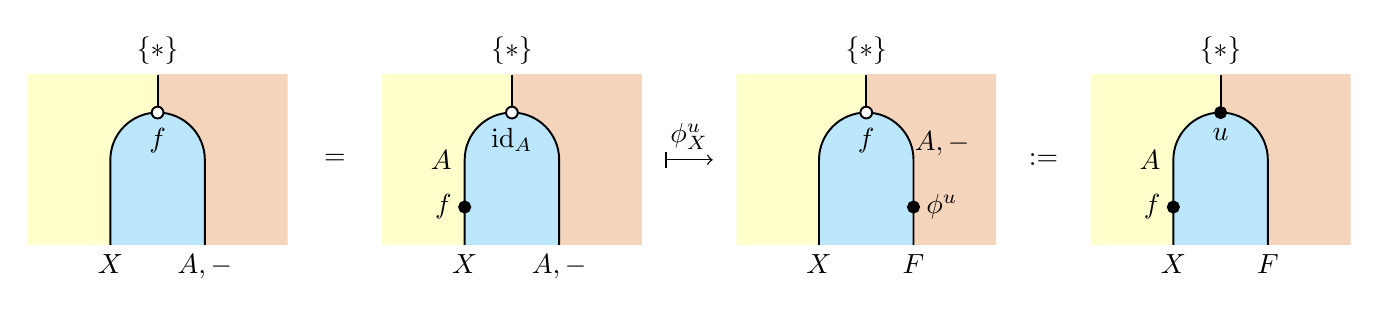
\begin{tikzpicture}[x=0.6cm,y=0.6cm, line width=0.7pt, hollow/.style={
            circle,
            fill=white,
            draw,
            outer sep=0pt,
            inner sep=1.5pt,
            line width=0.7pt
          }]
        % Define colors
    \definecolor{leftcolor}{RGB}{255,255,204}
    \definecolor{midcolor}{HTML}{BBE6FB}
    \definecolor{rightcolor}{HTML}{F5D4BC}

    \node at (-3.75, 1.8) {$=$};
    \draw [|-To, line width=0.5pt] (3.25,1.8) -- (4.25,1.8) node[midway,above] {$\phi^u_X$};
    \node at (11.25, 1.8) {$:=$};

    \begin{scope}[shift={(-7.5,0)}]
        \begin{scope} 
            \clip (-2.75,0) rectangle (2.75, 3.6);     
            \fill[fill=leftcolor] (-3,0) rectangle (0, 4);  
            \fill[fill=rightcolor] (0,0) rectangle (3, 4);  
            \draw[fill=midcolor, rounded corners=0.6cm, line width=0.7pt] (-1, -2) rectangle (1, 2.8);
        \end{scope}
        \draw (0, 3.6) -- (0,2.8);
        \node[below] at (-1, 0) {$X$};
        \node[below] at (1, 0) {$\llbracket A , -\rrbracket$};
        \node[hollow] at (0, 2.8) {};
        \node[below=2pt] at (0, 2.8) {$f$}; 
        \node[above] at (0, 3.6) {$\{*\}$};
    \end{scope}

    \begin{scope}[shift={(0,0)}]
        \begin{scope} 
            \clip (-2.75,0) rectangle (2.75, 3.6);     
            \fill[fill=leftcolor] (-3,0) rectangle (0, 4);  
            \fill[fill=rightcolor] (0,0) rectangle (3, 4);  
            \draw[fill=midcolor, rounded corners=0.6cm, line width=0.7pt] (-1, -2) rectangle (1, 2.8);
        \end{scope}
        \draw (0, 3.6) -- (0,2.8);
        \filldraw [black] (-1,0.8) circle (2pt) node[left=1pt] {$f$};
        \node[below] at (-1, 0) {$X$};
        \node[left=1pt] at (-1, 1.8) {$A$};
        \node[below] at (1, 0) {$\llbracket A , -\rrbracket$};
        \node[hollow] at (0, 2.8) {};
        \node[below=2pt] at (0, 2.8) {$\mathrm{id}_A$}; 
        \node[above] at (0, 3.6) {$\{*\}$};
    \end{scope}

    \begin{scope}[shift={(7.5,0)}]
       \begin{scope} 
            \clip (-2.75,0) rectangle (2.75, 3.6);     
            \fill[fill=leftcolor] (-3,0) rectangle (0, 4);  
            \fill[fill=rightcolor] (0,0) rectangle (3, 4);  
            \draw[fill=midcolor, rounded corners=0.6cm, line width=0.7pt] (-1, -2) rectangle (1, 2.8);
        \end{scope}
        \draw (0, 3.6) -- (0,2.8);
        \filldraw [black] (1,0.8) circle (2pt) node[right=1pt] {$\phi^u$};
        \node[below] at (-1, 0) {$X$};
        \node[right=-1.5pt] at (0.9, 2.15) {$\llbracket A , -\rrbracket$};
        \node[below] at (1, 0) {$F$};
        \node[hollow] at (0, 2.8) {};
        \node[below=2pt] at (0, 2.8) {$f$}; 
        \node[above] at (0, 3.6) {$\{*\}$};
    \end{scope}
    
    \begin{scope}[shift={(15,0)}]
       \begin{scope} 
            \clip (-2.75,0) rectangle (2.75, 3.6);     
            \fill[fill=leftcolor] (-3,0) rectangle (0, 4);  
            \fill[fill=rightcolor] (0,0) rectangle (3, 4);  
            \draw[fill=midcolor, rounded corners=0.6cm, line width=0.7pt] (-1, -2) rectangle (1, 2.8);
        \end{scope}
        \draw (0, 3.6) -- (0,2.8);
        \filldraw [black] (-1,0.8) circle (2pt) node[left=1pt] {$f$};
        \filldraw [black] (0, 2.8) circle (2pt) node[below=2pt] {$u$};
        \node[below] at (-1, 0) {$X$};
        \node[left=1pt] at (-1, 1.8) {$A$};
        \node[below] at (1, 0) {$F$};
        \node[above] at (0, 3.6) {$\{*\}$};
    \end{scope}
    \end{tikzpicture}
\]

\noindent and check that the naturality of $\phi^u$ as follows

\[
    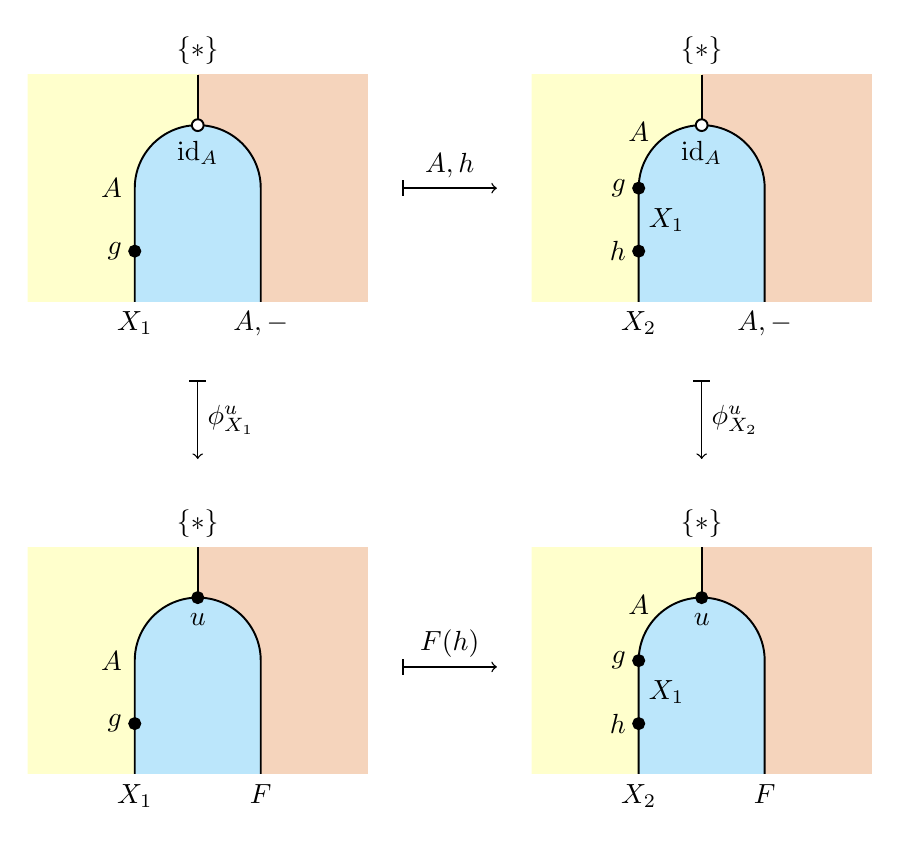
\begin{tikzpicture}[x=0.8cm,y=0.8cm, line width=0.7pt, hollow/.style={
            circle,
            fill=white,
            draw,
            outer sep=0pt,
            inner sep=1.5pt,
            line width=0.7pt
          }]
        % Define colors
         \definecolor{leftcolor}{RGB}{255,255,204}
    \definecolor{midcolor}{HTML}{BBE6FB}
    \definecolor{rightcolor}{HTML}{F5D4BC}

    \draw [|-To, line width=0.5pt] (-4.75,-5.8) -- (-3.25,-5.8) node[midway,above] {$F(h)$};
    \draw [|-To, line width=0.5pt] (0,-1.25) -- (0,-2.5) node[midway,right] {$\phi^u_{X_2}$};
    \draw [|-To, line width=0.5pt] (-4.75,1.8) -- (-3.25,1.8) node[midway,above] {$\llbracket A , h\rrbracket$};
    \draw [|-To, line width=0.5pt] (-8,-1.25) -- (-8,-2.5) node[midway,right] {$\phi^u_{X_1}$};  

    \begin{scope}[shift={(-8,0)}]
        \begin{scope} 
            \clip (-2.7,0) rectangle (2.7, 3.6);     
            \fill[fill=leftcolor] (-3,0) rectangle (0, 4);  
            \fill[fill=rightcolor] (0,0) rectangle (3, 4);  
            \draw[fill=midcolor, rounded corners=0.8cm, line width=0.7pt] (-1, -2) rectangle (1, 2.8);
        \end{scope}
        \draw (0, 3.6) -- (0,2.8);
        \filldraw [black] (-1,0.8) circle (2pt) node[left=1pt] {$g$};
        \node[below] at (-1, 0) {$X_1$};
        \node[left=1pt] at (-1, 1.8) {$A$};
        \node[below] at (1, 0) {$\llbracket A , -\rrbracket$};
        \node[hollow] at (0, 2.8) {};
        \node[below=2pt] at (0, 2.8) {$\mathrm{id}_A$}; 
        \node[above] at (0, 3.6) {$\{*\}$};
    \end{scope}

    \begin{scope}[shift={(-8,-7.5)}]
       \begin{scope} 
            \clip (-2.7,0) rectangle (2.7, 3.6);     
            \fill[fill=leftcolor] (-3,0) rectangle (0, 4);  
            \fill[fill=rightcolor] (0,0) rectangle (3, 4);  
            \draw[fill=midcolor, rounded corners=0.8cm, line width=0.7pt] (-1, -2) rectangle (1, 2.8);
        \end{scope}
        \draw (0, 3.6) -- (0,2.8);
        \filldraw [black] (-1,0.8) circle (2pt) node[left=1pt] {$g$};
        \filldraw [black] (0, 2.8) circle (2pt) node[below=2pt] {$u$};
        \node[below] at (-1, 0) {$X_1$};
        \node[left=1pt] at (-1, 1.8) {$A$};
        \node[below] at (1, 0) {$F$};
        \node[above] at (0, 3.6) {$\{*\}$};
    \end{scope}

    \begin{scope}[shift={(0,-7.5)}]
        \begin{scope} 
            \clip (-2.7,0) rectangle (2.7, 3.6);     
            \fill[fill=leftcolor] (-3,0) rectangle (0, 4);  
            \fill[fill=rightcolor] (0,0) rectangle (3, 4);  
            \draw[fill=midcolor, rounded corners=0.8cm, line width=0.7pt] (-1, -2) rectangle (1, 2.8);
        \end{scope}
        \draw (0, 3.6) -- (0,2.8);
        \node[below] at (-1, 0) {$X_2$};
        \node[right] at (-1, 1.3) {$X_1$};
        \node[below] at (-1, 3) {$A$};
        \node[below] at (1, 0) {$F$};
        % \node[hollow] at (0, 2.8) {};
        % \node[below=2pt] at (0, 2.8) {$u$}; 
        \filldraw [black] (-1,1.8) circle (2pt) node[left=1pt] {$g$};
        \filldraw [black] (-1,0.8) circle (2pt) node[left=1pt] {$h$};
        \filldraw [black] (0, 2.8) circle (2pt) node[below=2pt] {$u$};
        \node[above] at (0, 3.6) {$\{*\}$};
    \end{scope}

     \begin{scope}[shift={(0,0)}]
        \begin{scope} 
            \clip (-2.7,0) rectangle (2.7, 3.6);     
            \fill[fill=leftcolor] (-3,0) rectangle (0, 4);  
            \fill[fill=rightcolor] (0,0) rectangle (3, 4);  
            \draw[fill=midcolor, rounded corners=0.8cm, line width=0.7pt] (-1, -2) rectangle (1, 2.8);
        \end{scope}
        \draw (0, 3.6) -- (0,2.8);
        \node[below] at (-1, 0) {$X_2$};
        \node[right] at (-1, 1.3) {$X_1$};
        \node[below] at (-1, 3) {$A$};
        \node[below] at (1, 0) {$\llbracket A , -\rrbracket$};
        \node[hollow] at (0, 2.8) {};
        \node[below=2pt] at (0, 2.8) {$\mathrm{id}_A$}; 
        \filldraw [black] (-1,1.8) circle (2pt) node[left=1pt] {$g$};
        \filldraw [black] (-1,0.8) circle (2pt) node[left=1pt] {$h$};
        \node[above] at (0, 3.6) {$\{*\}$};
    \end{scope}
    
    \end{tikzpicture}    
\]
Then it is straightforward to see $\phi^u_{A}\left(\mathrm{id_A}\right)=u$ and $\phi^{\phi_A(\mathrm{id}_A)}=\phi$.


\cor{Yoneda Embedding}{
    Let $\mathsf{C}$ be a locally small category. The \hyperref[th:yoneda_embedding_functor]{Yoneda embedding functor} $Y_\mathsf{C}:\mathsf{C}\to \left[\mathsf{C}^{\mathrm{op}},\mathsf{Set}\right]$ is fully faithful. That is, for any $A_1,A_2\in\mathrm{Ob}\left(\mathsf{C}\right)$, the morphism set map 
    \begin{align*}
        \left.Y_{\mathsf{C}}\right|_{\operatorname{Hom}_{\mathsf{C}}\left(A_1,A_2\right)}:\operatorname{Hom}_{\mathsf{C}}\left(A_1,A_2\right) &\longrightarrow\operatorname{Hom}_{\mathsf{Psh}(\mathsf{C})}\left(\operatorname{Hom}_{\mathsf{C}}\left(-,A_1\right), \operatorname{Hom}_{\mathsf{C}}\left(-,A_2\right)\right) \\
         f & \longmapsto f_\star
    \end{align*}
    is a bijection. That justifies the name ``embedding'' because $\mathsf{C}$ is embedded into $\mathsf{Psh}(\mathsf{C})$ via $Y_\mathsf{C}$ as a full subcategory.
}
\pf{
    By \hyperref[th:yoneda_lemma]{Yoneda lemma}, there is a natural bijection
    \[
        \operatorname{Hom}_{\mathsf{Psh}(\mathsf{C})}\left(\operatorname{Hom}_{\mathsf{C}}\left(-,A_1\right), \operatorname{Hom}_{\mathsf{C}}\left(-,A_2\right)\right)\cong \operatorname{Hom}_{\mathsf{C}}\left(A_1,A_2\right),
    \]
    which is given by
    \begin{align*}
        r_{A_1,Y_{\mathsf{C}}(A_2)}:  \operatorname{Hom}_{\mathsf{C}}\left(A_1,A_2\right) &\xlongrightarrow{\sim}\operatorname{Hom}_{\mathsf{Psh}(\mathsf{C})}\left(\operatorname{Hom}_{\mathsf{C}}\left(-,A_1\right), \operatorname{Hom}_{\mathsf{C}}\left(-,A_2\right)\right) \\
         f & \longmapsto f_\star:\left[\begin{aligned}\left(f_\star\right)_X: \mathrm{Hom}_{\mathsf{C}}(X,A_1)&\longrightarrow \mathrm{Hom}_{\mathsf{C}}(X,A_2)\\
             g&\longmapsto f_*(g)=f\circ g\end{aligned}  \right]
    \end{align*}
    and
    \begin{align*}
        q_{A_1,Y_{\mathsf{C}}(A_2)}:\operatorname{Hom}_{\mathsf{Psh}(\mathsf{C})}\left(\operatorname{Hom}_{\mathsf{C}}\left(-,A_1\right), \operatorname{Hom}_{\mathsf{C}}\left(-,A_2\right)\right) & \xlongrightarrow{\sim}\operatorname{Hom}_{\mathsf{C}}\left(A_1,A_2\right) \\
        {  \left[ \begin{tikzcd}[ampersand replacement=\&]
            \mathsf{C}^{\mathrm{op}} \arrow[r, "\operatorname{Hom}_{\mathsf{C}}\left(-{,}A_1\right)"{name=A, above}, bend left] \arrow[r, "\operatorname{Hom}_{\mathsf{C}}\left(-{,}A_2\right)"'{name=B, below}, bend right] \&[+30pt] \mathsf{Set}
            \arrow[Rightarrow, shorten <=5.5pt, shorten >=5.5pt, from=A.south-|B, to=B, "\phi"]
        \end{tikzcd}\right] } & \longmapsto \phi_{A_1}\left(\operatorname{id}_{A_1}\right)
    \end{align*}
    Note that $r_{A_1,Y_{\mathsf{C}}(A_2)}$ is exactly the morphism set map $\left.Y_{\mathsf{C}}\right|_{\operatorname{Hom}_{\mathsf{C}}\left(A_1,A_2\right)}$.
}
Yoneda embedding allows us to regard any category $\mathsf{C}$ as a full subcategory of $\mathsf{Psh}(\mathsf{C})$. So in the sense of categorical isomorphism, we can identify any object $A\in \mathrm{Ob}(\mathsf{C})$ with a presheaf $\operatorname{Hom}_{\mathsf{C}}(-, A)$. 

An object in a category is equivalent to the collection of all arrows pointing to that object. In other words, the information we care about is which arrows from an object itself and other objects would point to this object, while the object's internals are completely regarded as a black box. 

The arrows between objects in a category are equivalent to the transformations between sets of arrows pointing to objects. Specifically, suppose $f$ is an arrow from object $A$ to object $B$, then any arrow pointing to $A$ can be transformed into an arrow pointing to $B$ by appending an $f$, which is exactly what $f_\star$ does. Conversely, if there is a way to naturally transform all arrows pointing to $A$ into arrows pointing to $B$, then this transformation must be realized by appending an arrow between $A$ and $B$.

\dfn{Representable Functor}{
    Let $\mathsf{C}$ be a locally small category. 
    \begin{itemize}
        \item A functor $F:\mathsf{C}\to \mathsf{Set}$ is called \textbf{representable} if it is naturally isomorphic to $\operatorname{Hom}_{\mathsf{C}}\left(A,-\right)$ for some $A\in \mathrm{Ob}(\mathsf{C})$.
        \item A functor $F:\mathsf{C}^{\mathrm{op}}\to \mathsf{Set}$ is called \textbf{representable} if it is naturally isomorphic to $\operatorname{Hom}_{\mathsf{C}}\left(-,A\right)$ for some $A\in \mathrm{Ob}(\mathsf{C})$.
    \end{itemize}
    A \textbf{representation of $F$} is a pair $(A,\phi)$, where $A\in \mathrm{Ob}(\mathsf{C})$ and $\phi:  \operatorname{Hom}_{\mathsf{C}}\left(A,-\right)\xRightarrow{\sim} F$ is a natural isomorphism. \\
    According to \hyperref[th:yoneda_lemma]{Yoneda lemma}, $\phi:\operatorname{Hom}_{\mathsf{C}}\left(A,-\right)\Rightarrow  F$ is 1-1 correspondence with an element $\phi_A(\mathrm{id}_A)\in F(A)$. We define an \textbf{universal element of $F$} is a pair $(A,u)$ where $A\in \mathrm{Ob}(\mathsf{C})$ and $u\in F(A)$ such that $u$ corresponds to a natural isomorphism $\phi: \operatorname{Hom}_{\mathsf{C}}\left(A,-\right)\xRightarrow{\sim} F$. Specifying a universal element of $F$ is equivalent to specifying a representation of $F$.
}
\[
 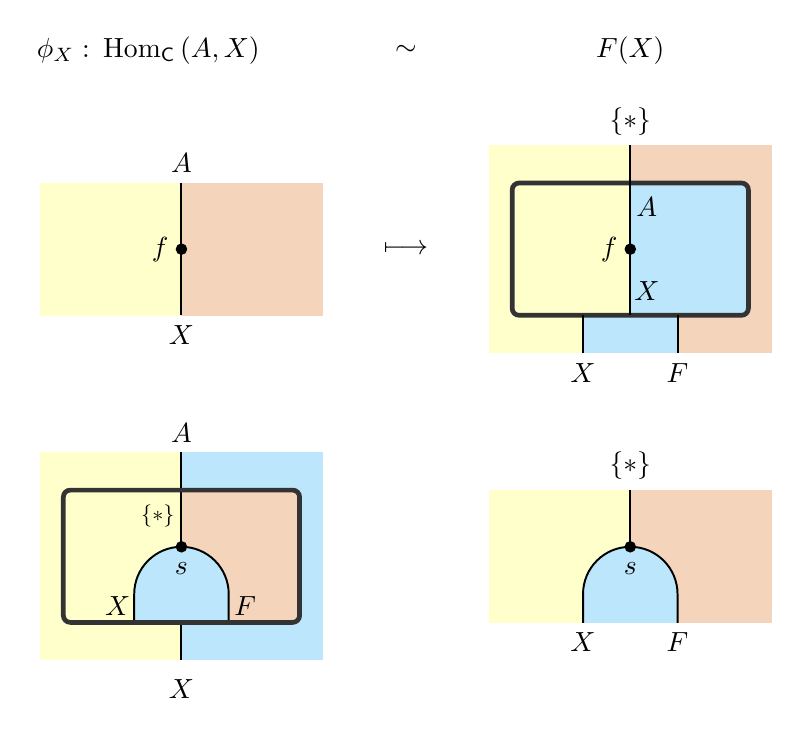
\begin{tikzpicture}[x=0.6cm,y=0.6cm, baseline=(current bounding box.center), line width=0.7pt]
    \definecolor{leftcolor}{RGB}{255,255,204}
    \definecolor{midcolor}{HTML}{BBE6FB}
    \definecolor{rightcolor}{HTML}{F5D4BC}
    \node at (-2.5, 6) {$\phi_{X}:$};
    \node at (0, 6) {$\mathrm{Hom}_{\mathsf{C}}\left(A,X\right)$};
    \node at (4.75, 6) {$\xlongrightarrow{\sim}$};
    \node at (4.75, -4.75) {$\longmapsfrom$};
    \node at (4.75, 1.8) {$\longmapsto$};
    \node at (9.5, 6) {$F(X)$};
    
    \begin{scope}[line width=0.7pt]
        \begin{scope}
            \clip (-3,0.4) rectangle (3,3.2);     
            \fill[fill=leftcolor] (-3,0) rectangle (0, 3.2);  
            \fill[fill=rightcolor] (0,0) rectangle (3, 3.2);  
        \end{scope}
        \node[below] at (0, 0.4) {$X$};
        \node[left=1pt] at (0, 1.8) {$f$};
        \draw[fill=black] (0, 1.8) circle (0.1);  
        \draw (0, 3.2) -- (0, 0.4);
        \node[above] at (0, 3.2) {$A$};
    \end{scope}

    \begin{scope}[shift={(9.5,0)}]
    \fill[fill=leftcolor] (-3,-0.4) rectangle (0,4); 
     \fill[fill=rightcolor] (0, -0.4) rectangle (3,4); 
     \fill[fill=midcolor] (-1, -0.4) rectangle (1,2); 
        \begin{scope} 
            \clip (-2.5,0.4) rectangle (2.5,3.2);     
            \fill[fill=leftcolor] (-2.5,0) rectangle (0, 3.2);  
            \fill[fill=midcolor] (0,0) rectangle (2.5, 3.2);  
        \end{scope}
        \draw[line width=1.7pt, color=black!80, rounded corners=2.5pt] (-2.5, 0.4) rectangle (2.5, 3.2); % inner rectangle
        \node[above,shift={(0.35,0.1)}] at (0, 0.4) {$X$};
        \node[left=1pt] at (0, 1.8) {$f$};
        \draw[fill=black] (0, 1.8) circle (0.1);  
        \draw (0, 4) -- (0, 0.4);
        \node[below,shift={(0.35,-0.1)}] at (0, 3.2) {$A$};
        \draw (1, 0.4) -- (1, -0.4);
        \draw (-1, 0.4) -- (-1, -0.4);
        \node[above] at (0, 4) {$\{*\}$};
        \node[below] at (-1, -0.4) {$X$};
        \node[below] at (1, -0.4) {$F$};
    \end{scope}
    
    \begin{scope}[shift={(0, -6.5)}, line width=0.7pt]
    \fill[fill=leftcolor] (-3,-0.4) rectangle (0,4); 
     \fill[fill=midcolor] (0, -0.4) rectangle (3,4); 
        \begin{scope} 
            \clip (-2.5,0.4) rectangle (2.5, 3.2);     
            \fill[fill=leftcolor] (-2.5,0) rectangle (0, 3.2);  
            \fill[fill=rightcolor] (0,0) rectangle (2.5, 3.2);  
            \draw[fill=midcolor, rounded corners=0.6cm] (-1, -2) rectangle (1, 2);
        \end{scope}
        \node[shift={(-0.35,0.35)}] at (-1, 0.4) {$X$};
        \node[shift={(0.35,0.35)}] at (1, 0.4) {$F$};
        \node[below=2pt] at (0, 2) {$s$};
        \draw[fill=black] (0, 2) circle (0.1);  
        \draw (0,4) -- (0,2);
        \draw (0, -0.4) -- (0,0.4);
        \node[below,shift={(-0.5,0.1)}] at (0, 3) {\scalebox{.8}{$\{*\}$}};
        \draw[line width=1.7pt, color=black!80, rounded corners=2.5pt] (-2.5, 0.4) rectangle (2.5, 3.2); % inner rectangle
        \node[above] at (0, 4){$A$};
        \node[below] at (0, -0.6){$X$};
    \end{scope}

    \begin{scope}[shift={(9.5, -6.5)}, line width=0.7pt]
        \begin{scope} 
            \clip (-3,0.4) rectangle (3,3.2);     
            \fill[fill=leftcolor] (-3,0) rectangle (0, 3.2);  
            \fill[fill=rightcolor] (0,0) rectangle (3, 3.2);  
            \draw[fill=midcolor, rounded corners=0.6cm] (-1, -2) rectangle (1, 2);
        \end{scope}
        \node[below] at (-1, 0.4) {$X$};
        \node[below] at (1, 0.4) {$F$};
        \node[below=2pt] at (0, 2) {$s$};
        \draw[fill=black] (0, 2) circle (0.1);  
        \draw (0,3.2) -- (0,2);
        \node[above] at (0, 3.2) {$\{*\}$};
    \end{scope}
    \end{tikzpicture}
\]

The naturality diagram of $\phi$ 
\[
    \begin{tikzcd}[ampersand replacement=\&, row sep = 3.5em]
        \mathrm{Hom}_{\mathsf{C}}(A,X) \arrow[d, "{\phi_X}"'{name=L, left}, "{\sim}"{name=R, right}]  \arrow[rr, "{h_*}"] \&[-20pt] \& {\mathrm{Hom}_{\mathsf{C}}(A,Y)} \arrow[d, "{\phi_Y}"'{name=L, right}, "{\sim}"{name=R, left}]\\
        {F(X)}\arrow[rr, "{F(h)}"'] \&  \& {F(Y)}  
    \end{tikzcd}
\]
can be translated into the following calculus rules

\[
 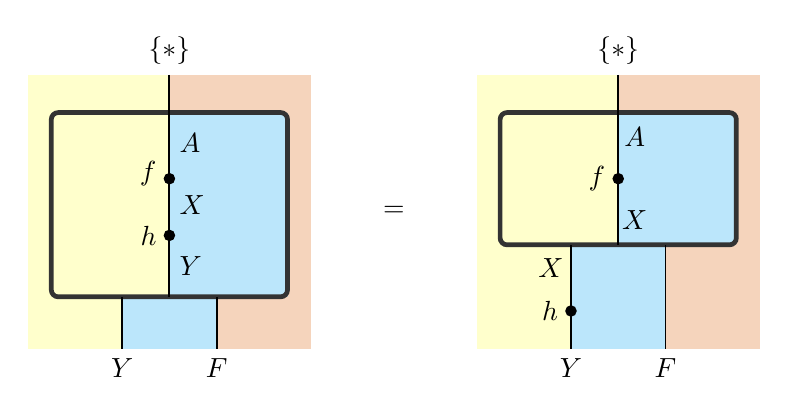
\begin{tikzpicture}[x=0.6cm,y=0.6cm, baseline=(current bounding box.center), line width=0.7pt]
    \definecolor{leftcolor}{RGB}{255,255,204}
    \definecolor{rightcolor}{HTML}{BBE6FB}
    \definecolor{midcolor}{HTML}{F5D4BC}

    \node at (4.75, 1.1) {$=$};
  
    \begin{scope}[shift={(9.5,0)}]
     \fill[fill=leftcolor] (-3,-1.8) rectangle (0,4); 
     \fill[fill=midcolor] (0, -1.8) rectangle (3,4); 
     \fill[fill=rightcolor] (-1, -1.8) rectangle (1,2); 
        \begin{scope} 
            \clip (-2.5,0.4) rectangle (2.5,3.2);     
            \fill[fill=leftcolor] (-2.5,0) rectangle (0, 3.2);  
            \fill[fill=rightcolor] (0,0) rectangle (2.5, 3.2);  
        \end{scope}
        \draw[line width=1.7pt, color=black!80, rounded corners=2.5pt] (-2.5, 0.4) rectangle (2.5, 3.2); % inner rectangle
        \node[above,shift={(0.35,0.1)}] at (0, 0.4) {$X$};
        \node[left=1pt] at (0, 1.8) {$f$};
        \draw[fill=black] (0, 1.8) circle (0.1);  
        \draw (0, 4) -- (0, 0.4);
        \node[below,shift={(0.35,-0.1)}] at (0, 3.2) {$A$};
        \draw (1, 0.4) -- (1, -1.8);
        \draw (-1, 0.4) -- (-1, -1.8);
        \node[above] at (0, 4) {$\{*\}$};
        \node[below] at (-1, -1.8) {$Y$};
        \node[below] at (1, -1.8) {$F$};
        \node[left=-1pt] at (-1, -0.1) {$X$};
        \filldraw [black] (-1, -1) circle (0.1) node[left=1pt] {$h$};
    \end{scope}

    \begin{scope}
    \fill[fill=leftcolor] (-3,-1.8) rectangle (0,4); 
     \fill[fill=midcolor] (0, -1.8) rectangle (3,4); 
     \fill[fill=rightcolor] (-1, -1.8) rectangle (1,2); 
        \begin{scope} 
            \clip (-2.5,-0.7) rectangle (2.5,3.2);     
            \fill[fill=leftcolor] (-2.5,-2) rectangle (0, 3.2);  
            \fill[fill=rightcolor] (0,-2) rectangle (2.5, 3.2);  
        \end{scope}
        \draw[line width=1.7pt, color=black!80, rounded corners=2.5pt] (-2.5, -0.7) rectangle (2.5, 3.2); % inner rectangle
        \node[right] at (0, 1.25) {$X$};
        \node[left=1pt] at (0, 1.9) {$f$};
        \draw[fill=black] (0, 1.8) circle (0.1);  
        \draw (0, 4) -- (0, -0.7);
        \node[right] at (0, 2.55) {$A$};
        \draw (1, -0.7) -- (1, -1.8);
        \draw (-1, -0.7) -- (-1, -1.8);
        \node[above] at (0, 4) {$\{*\}$};
        \node[below] at (-1, -1.8) {$Y$};
        \node[below] at (1, -1.8) {$F$};
        \node[right] at (0, -0.05) {$Y$};
        \filldraw [black] (0, 0.6) circle (0.1) node[left=1pt] {$h$};
    \end{scope}
   
    \end{tikzpicture}
\]
\[
 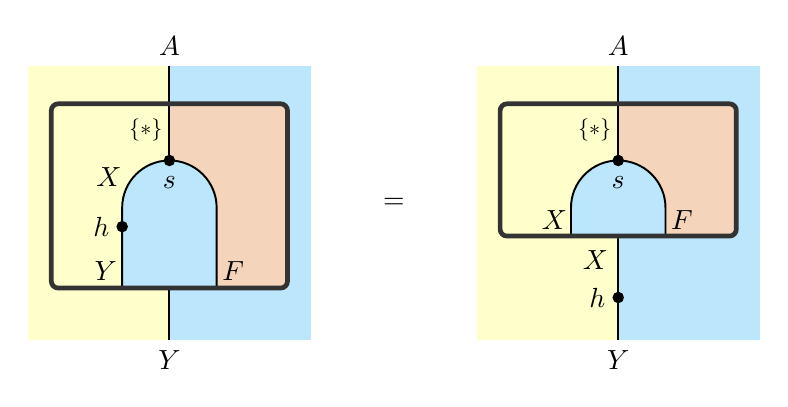
\begin{tikzpicture}[x=0.6cm,y=0.6cm, baseline=(current bounding box.center), line width=0.7pt]
    \definecolor{leftcolor}{RGB}{255,255,204}
    \definecolor{rightcolor}{HTML}{BBE6FB}
    \definecolor{midcolor}{HTML}{F5D4BC}

    \node at (4.75, 1.1) {$=$};
  
    \begin{scope}[shift={(9.5,0)}]
   \fill[fill=leftcolor] (-3,-1.8) rectangle (0,4); 
     \fill[fill=rightcolor] (0, -1.8) rectangle (3,4); 
        \begin{scope} 
            \clip (-2.5,0.4) rectangle (2.5, 3.2);     
            \fill[fill=leftcolor] (-2.5,0) rectangle (0, 3.2);  
            \fill[fill=midcolor] (0,0) rectangle (2.5, 3.2);  
            \draw[fill=rightcolor, rounded corners=0.6cm] (-1, -2) rectangle (1, 2);
        \end{scope}
        \node[shift={(-0.35,0.35)}] at (-1, 0.4) {$X$};
        \node[shift={(0.35,0.35)}] at (1, 0.4) {$F$};
        \node[below=2pt] at (0, 2) {$s$};
        \draw[fill=black] (0, 2) circle (0.1);  
        \draw (0,4) -- (0,2);
        \draw (0, -1.8) -- (0,0.4);
        \node[below,shift={(-0.5,0.1)}] at (0, 3) {\scalebox{.8}{$\{*\}$}};
        \draw[line width=1.7pt, color=black!80, rounded corners=2.5pt] (-2.5, 0.4) rectangle (2.5, 3.2); % inner rectangle
        \node[above] at (0, 4){$A$};
        \node[left] at (0, -0.1){$X$};
        \node[below] at (0, -1.8){$Y$};
        \filldraw [black] (0, -0.9) circle (0.1) node[left=1pt] {$h$};
    \end{scope}

    \begin{scope}
   \fill[fill=leftcolor] (-3,-1.8) rectangle (0,4); 
     \fill[fill=rightcolor] (0, -1.8) rectangle (3,4); 
        \begin{scope} 
            \clip (-2.5,-0.7) rectangle (2.5, 3.2);     
            \fill[fill=leftcolor] (-2.5,0) rectangle (0, 3.2);  
            \fill[fill=midcolor] (0,-1) rectangle (2.5, 3.2);  
            \draw[fill=rightcolor, rounded corners=0.6cm] (-1, -2) rectangle (1, 2);
        \end{scope}
        \node[shift={(-0.35,0.35)}] at (-1, -0.7) {$Y$};
        \node[shift={(0.35,0.35)}] at (1, -0.7) {$F$};
        \node[below=2pt] at (0, 2) {$s$};
        \draw[fill=black] (0, 2) circle (0.1);  
        \draw (0,4) -- (0,2);
        \draw (0, -1.8) -- (0, -0.7);
        \node[below,shift={(-0.5,0.1)}] at (0, 3) {\scalebox{.8}{$\{*\}$}};
        \draw[line width=1.7pt, color=black!80, rounded corners=2.5pt] (-2.5, -0.7) rectangle (2.5, 3.2); % inner rectangle
        \node[above] at (0, 4){$A$};
        \node[left] at (-0.8, 1.65){$X$};
        \node[below] at (0, -1.8){$Y$};
        \filldraw [black] (-1, 0.6) circle (0.1) node[left=1pt] {$h$};
    \end{scope}   
    \end{tikzpicture}
\]


\prop[representable_functor_by_universal_element]{Equivalent Characterizations of Representable Functor}{
    Suppose $F:\mathsf{C}\to \mathsf{Set}$ is a functor. Then the following statements are equivalent:
    \begin{enumerate}[(i)]
        \item $F$ is representable by universal element $(A,u)$ 
        \item $(A,u)$ is initial in the category \hyperref[th:category_of_elements]{$\int_{\mathsf{C}}F$}$=\left(\{*\} \downarrow F\right)$, which corresponds to $ \begin{tikzcd}[ampersand replacement=\&]
            \mathsf{1} \arrow[r, "\diagfunctor\{*\}"] \& \mathsf{Set} \& \mathsf{C}  \arrow[l, " F"']
        \end{tikzcd}$.
        \item $(A,\phi^u)$ is initial in the category $\left(  \text{\hyperref[th:yoneda_embedding_functor]{$Y_{\mathsf{C}^{\mathrm{op}}}$}}\downarrow F\right)$, which corresponds to $ \begin{tikzcd}[ampersand replacement=\&]
           \mathsf{C}^{\mathrm{op}}  \arrow[r, " Y_{\mathsf{C}^{\mathrm{op}}}"] \& \left[\mathsf{C},\mathsf{Set}\right] \&  \mathsf{1} \arrow[l, "\diagfunctor F"']
        \end{tikzcd}$.
        \item $\left(A,\diagfunctor u:\{*\}\to F(A)\right)$ is a \hyperref[th:universal_morphism]{universal morphism} from $\{*\}$ to $F$.
        \item For any $(X,x)\in \mathrm{Ob}(\int_{\mathsf{C}}F)$, there is a unique morphism $(A,u)\to (X,x)$ in $\int_{\mathsf{C}}F$ (which is a morphism $f:A\to X$ in $\mathsf{C}$ such that $F(f)(u)=x$).
    \end{enumerate}
    Suppose $F:\mathsf{C}^{\mathrm{op}}\to \mathsf{Set}$ is a functor. Then the following statements are equivalent:
    \begin{enumerate}[(i)]
        \item $F$ is representable by universal element $(A,u)$ 
        \item $(A,u)$ is initial in the category \hyperref[th:category_of_elements]{$\int_{\mathsf{C}^{\mathrm{op}}}F$}$=\left(\{*\} \downarrow F\right)$, which corresponds to $ \begin{tikzcd}[ampersand replacement=\&]
            \mathsf{1} \arrow[r, "\diagfunctor\{*\}"] \& \mathsf{Set} \& \mathsf{C}^{\mathrm{op}}  \arrow[l, " F"']
        \end{tikzcd}$.
        \item $(A,\phi^u)$ is terminal in the category $\left(  \text{\hyperref[th:yoneda_embedding_functor]{$Y_{\mathsf{C}}$}}\downarrow F\right)$, which corresponds to $ \begin{tikzcd}[ampersand replacement=\&]
           \mathsf{C} \arrow[r, " Y_{\mathsf{C}}"] \& \left[\mathsf{C}^{\mathrm{op}},\mathsf{Set}\right] \&  \mathsf{1} \arrow[l, "\diagfunctor F"']
        \end{tikzcd}$.
        \item $\left(A,\diagfunctor u:\{*\}\to F(A)\right)$ is a \hyperref[th:universal_morphism]{universal morphism} from $\{*\}$ to $F$.
        \item For any $(X,x)\in \mathrm{Ob}\left(\int_{\mathsf{C}^{\mathrm{op}} }F\right)$, there is a unique morphism $(A,u)\to (X,x)$ in $\int_{\mathsf{C}^{\mathrm{op}} }F$ (which is a morphism $f: X\to A$ in $\mathsf{C}$ such that $F(f)(x)=u$).
    \end{enumerate}
}
\pf{
    (i)$\iff$ (ii). Suppose $(A,u)$ is an object of $\int_{\mathsf{C}}F$ and $\phi^u:\operatorname{Hom}_{\mathsf{C}}\left(A,-\right)\Rightarrow F$ be the natural transformation
    \[
        \phi^u_X(f)=F(f)(u),\quad\forall f\in \mathrm{Hom}_{\mathsf{C}}(A,X),
    \]
    which can be illustrated by the following diagram
    \[
		\begin{tikzcd}[ampersand replacement=\&, row sep = 3.5em]
			\mathrm{id}_A\arrow[d, mapsto]\&[-25pt]\in\&[-25pt]\mathrm{Hom}_{\mathsf{C}}(A,A) \arrow[d, "{\phi_A^u}"']  \arrow[rr, "{f_*}"] \&[-20pt] \& {\mathrm{Hom}_{\mathsf{C}}(A,X)} \arrow[d, "\phi_X^u"]\&[-25pt]\ni\&[-25pt]f \arrow[d, mapsto]\\
			u=\phi_A^u(\mathrm{id}_A)\&\in\&{F(A)}\arrow[rr, "{F(f)}"'] \&  \& {F(X)}  \&\ni\& \phi_X^u(f)     
		\end{tikzcd}
	\]   
    Thus we have
    \begin{align*}
        (A,u)\text{ is initial in }\int_{\mathsf{C}}F&\iff \forall(X,x)\in \mathrm{Ob}\left(\int_{\mathsf{C}}F\right),\;\exists! f\in \mathrm{Hom}_{\mathsf{C}}(A,X),\;F(f)(u)=x\\
        &\iff\forall X\in \mathrm{Ob}\left(\mathsf{C}\right),\; \forall x\in F(X),\;\exists! f\in \mathrm{Hom}_{\mathsf{C}}(A,X),\;\phi_X^u(f)=x\\
        &\iff \forall X\in \mathrm{Ob}\left(\mathsf{C}\right),\;\phi_X^u \text{ is bijective}\\
        &\iff \phi^u \text{ is a natural isomorphism}\\
        &\iff (A,u) \text{ is a universal element of }F.
    \end{align*}
    \[
        \begin{tikzcd}[ampersand replacement=\&, row sep=9pt]
              \& F(A) \arrow[dd, dashed, "F(f)"]\\
            \{*\}\arrow[ru, "\diagfunctor u"]\arrow[rd, "\diagfunctor x"']\& \\
             \& F\left(X\right)
            \end{tikzcd}
    \]
    (i)$\iff$ (iii). $\left(A,\phi^u\right)$ is initial in $\left(  Y_{\mathsf{C}^{\mathrm{op}}}\downarrow F\right)$ if and only if for any $ X\in \mathrm{Ob}\left(\mathsf{C}\right)$ and any natural transformation $\psi:\mathrm{Hom}_\mathsf{C}\left(X,-\right)\implies F$, there is a unique $f\in \mathrm{Hom}_{\mathsf{C}}(A,X)$ such that $\phi^u\circ f^\star=\psi$
    \[
        \begin{tikzcd}[ampersand replacement=\&, row sep=9pt]
               \mathrm{Hom}_{\mathsf{C}}\left(A,-\right) \arrow[rd, "\phi^u"]\&\\
            \& F\\
             \mathrm{Hom}_{\mathsf{C}}\left(X,-\right) \arrow[ru, "\psi"']\arrow[uu, dashed, "f^\star"]\& 
            \end{tikzcd}
    \]
    or equivalently
    \[
        \psi_X(\mathrm{id}_X)=\left(\phi^u\circ f^\star\right)_X(\mathrm{id}_X)=\phi^u_X(f).
    \]
    Suppose $F$ is representable by universal element $(A,u)$. Then $\phi^u:\mathrm{Hom}_\mathsf{C}\left(A,-\right)\xRightarrow{\sim} F$ is a natural isomorphism. Since
    \begin{align*}
        \left.Y_{\mathsf{C}^{\mathrm{op}}}\right|_{\operatorname{Hom}_{\mathsf{C}}\left(A,X\right)}:\operatorname{Hom}_{\mathsf{C}}\left(A,X\right) &\xlongrightarrow{\sim}\operatorname{Hom}_{[\mathsf{C},\mathsf{Set}]}\left(\operatorname{Hom}_{\mathsf{C}}\left(X,-\right), \operatorname{Hom}_{\mathsf{C}}\left(A,-\right)\right) \\
         f & \longmapsto f^\star
    \end{align*}
    is a bijection, there is a unique $f\in \mathrm{Hom}_{\mathsf{C}}(A,X)$ such that $f^\star=\left(\phi^u\right)^{-1}\circ\psi$ or equivalently $\phi^u\circ f^\star=\psi$.

    Conversely, suppose $(A,\phi^u)$ is initial in $\left(  Y_{\mathsf{C}^{\mathrm{op}}}\downarrow F\right)$. Then for any $ X\in \mathrm{Ob}\left(\mathsf{C}\right)$ and any $x\in F(X)$, there exist natural transformation $\psi^x:\mathrm{Hom}_\mathsf{C}\left(X,-\right)\implies F$ and unique $f\in \mathrm{Hom}_{\mathsf{C}}(A,X)$ such that $x=\psi_X^x(\mathrm{id}_X)=\phi^u_X(f)$,
    \[
        \begin{tikzcd}[ampersand replacement=\&, row sep=9pt]
               \mathrm{Hom}_{\mathsf{C}}\left(A,X\right) \arrow[rd, "\phi^u_X"]\&\\
            \& F(X)\\
             \mathrm{Hom}_{\mathsf{C}}\left(X,X\right) \arrow[ru, "\psi_X^x"']\arrow[uu, dashed, "f^*"]\& 
            \end{tikzcd}
    \]
    which implies $\phi^u_X$ is bijective. Thus $\phi^u$ is a natural isomorphism and $(A,u)$ is a universal element of $F$.
}
\cor[initial_object_representable_functor]{Initial Object Characterized by Representable Functor}{
    Suppose $\mathsf{C}$ is a locally small category.
    \begin{itemize}
        \item $A\in\mathrm{Ob}(\mathsf{C})$ is initial in $\mathsf{C}$ if and only if the functor $\diagfunctor \{*\}:\mathsf{C}\to \mathsf{Set}$ is naturally isomorphic to $\mathrm{Hom}_\mathsf{C}\left(A,-\right)$.
        \item $A\in\mathrm{Ob}(\mathsf{C})$ is terminal in $\mathsf{C}$ if and only if the functor $\diagfunctor \{*\}:\mathsf{C}^{\mathrm{op}}\to \mathsf{Set}$ is naturally isomorphic to $\mathrm{Hom}_\mathsf{C}\left(-,A\right)$.
    \end{itemize}
}
\pf{
    Let $\diagfunctor \{*\}:\mathsf{C}\to \mathsf{Set}$ be a constant functor. It is easy to see that the category $\int_\mathsf{C}\diagfunctor \{*\}$ is isomorphic to $\mathsf{C}$ through the functor
    \begin{align*}
        p:\int_\mathsf{C}\diagfunctor \{*\}&\longrightarrow \mathsf{C}\\
        (C,*) &\longmapsto C
    \end{align*}
    As established in \Cref{th:representable_functor_by_universal_element},
    $(A,*)\in\mathrm{Ob}(\mathsf{C})$ is initial in $\int_\mathsf{C}\diagfunctor \{*\}$ if and only if $\diagfunctor \{*\}$ is a representable functor with a universal element $(A,*)$, which proves the first statement. The second statement can be obtained by applying the first statement to $\mathsf{C}^{\mathrm{op}}$.\\
    In addition, an alternative ad-hoc proof is conceivable. If $\diagfunctor \{*\}$ is naturally isomorphic to $\mathrm{Hom}_\mathsf{C}\left(A,-\right)$ through $\theta:\mathrm{Hom}_\mathsf{C}\left(A,-\right)\xRightarrow{\sim} \diagfunctor \{*\}$, we have no choice but to define $\theta_X(\mathrm{id}_X)=*$. Note that $\diagfunctor \{*\}(A)=\{*\}$.  Yoneda lemma also implies that $\theta$ must correspond to $*\in \diagfunctor \{*\}(A)$ and accordingly $\theta$ is the unique natural isomorphism from $\mathrm{Hom}_\mathsf{C}\left(A,-\right)$ to $\diagfunctor\{*\}$.
}

\prop[universal_morphism_by_representability]{Equivalent Characterizations of Universal Morphism}{
    Let $F:\mathsf{C}\to \mathsf{D}$ be a functor and $A\in \mathrm{Ob}(\mathsf{D})$. Then the following statements are equivalent:
    \begin{enumerate}[(i)]
        \item $(A,u)$ is initial in the category $\left(X \downarrow F\right)$.
        \item $\mathrm{Hom}_{\mathsf{D}}\left(X,F(-)\right)$ is representable by universal element $(A,u)$.
        \item $(A,u)$ is initial in the category $\int_{\mathsf{C}}  \mathrm{Hom}_{\mathsf{D}}\left(X,F(-)\right)=\left( \{*\}\downarrow \mathrm{Hom}_{\mathsf{D}}\left(X,F(-)\right)\right)$.
    \end{enumerate}
 Dually, the following statements are equivalent:
    \begin{enumerate}[(i)]
        \item $(A,u)$ is terminal in the category $\left(F \downarrow X\right)$.
        \item $\mathrm{Hom}_{\mathsf{D}}\left(F(-),X\right)$ is representable by universal element $(A,u)$.
        \item $(A,u)$ is initial in the category $\int_{\mathsf{C}^{\mathrm{op}}}  \mathrm{Hom}_{\mathsf{D}}\left(F(-),X\right)=\left( \{*\}\downarrow \mathrm{Hom}_{\mathsf{D}}\left(F(-),X\right)\right)$.
    \end{enumerate}
}
\pf{     
    It suffices to show (i)$\iff$ (iii).
    \[
    \begin{tikzcd}[ampersand replacement=\&]
        X \arrow[r, "u"] \arrow[rd, "g"'] \&[+20pt] F(A) \arrow[d, "F\left(h\right)", dashed]\&[+50pt] \{*\} \arrow[r, "\diagfunctor u"] \arrow[rd, "\diagfunctor g"'] \&[+15pt] \mathrm{Hom}_{\mathsf{D}}\left(X,F(A)\right)\arrow[d, "F(h)_*", dashed] \\[+15pt]\& F(B)\&\&\mathrm{Hom}_{\mathsf{D}}\left(X,F(B)\right)                                              
    \end{tikzcd}
    \]
    \begin{align*}
        (A,u)\text{ is initial in }\left(X \downarrow F\right)&\iff \forall(B,g)\in \mathrm{Ob}\left(X \downarrow F\right),\;\exists! h\in \mathrm{Hom}_{\mathsf{C}}(A,B),\;F(h)\circ u=g\\
        &\iff \forall B\in \mathrm{Ob}\left(\mathsf{C}\right),\;\forall g\in \mathrm{Hom}_{\mathsf{C}}(X,F(B)),\;\exists! h\in \mathrm{Hom}_{\mathsf{C}}(A,B),\;F(h)\circ u=g\\
        &\iff \forall (B,\diagfunctor g)\in \mathrm{Ob}\left(\int_{\mathsf{C}}  \mathrm{Hom}_{\mathsf{D}}\left(X,F(-)\right)\right),\;\exists! h\in \mathrm{Hom}_{\mathsf{C}}(A,B),\;F(h)_*\circ\diagfunctor u=\diagfunctor g\\
        &\iff (A,u)\text{ is initial in }\int_{\mathsf{C}}  \mathrm{Hom}_{\mathsf{D}}\left(X,F(-)\right)
    \end{align*}
  The dual version is similar.

}

\section{Limit and Colimit}
\dfn[cone]{Cone}{
    Let $\mathsf{J},\mathsf{C}$ be categories and $F:\mathsf{J}\to\mathsf{C}$ be a functor. Consider functors
    \[
        \begin{tikzcd}[ampersand replacement=\&]
            \mathsf{C} \arrow[r, "\diagfunctor"] \& {[\mathsf{J},\mathsf{C}]} \& \mathsf{1} \arrow[l, "\diagfunctor F"']
        \end{tikzcd}
    \]
    The comma category $\left(\diagfunctor \downarrow \diagfunctor F\right)$ is called the \textbf{cone category from $\textsf{C}$ to $F$}, denoted by $\mathsf{Cone}(\textsf{C},F)$. 
    \begin{itemize}
        \item Objects: The objects in $\mathsf{Cone}(\textsf{C},F)$ are all natural transformations 
        \[
                \begin{tikzcd}[ampersand replacement=\&]
                    \mathsf{J} \arrow[r, "\diagfunctor C"{name=A, above}, bend left] \arrow[r, "F"'{name=B, below}, bend right] \&[+30pt] \mathsf{C}
                    \arrow[Rightarrow, shorten <=5.5pt, shorten >=5.5pt, from=A.south-|B, to=B, "h"]
                \end{tikzcd}
        \]
        where $C\in \mathrm{Ob}(\mathsf{C})$. Such $h:\diagfunctor C\Rightarrow F$ is called a \textbf{cone from $C$ to $F$} because it can be viewed as a family of morphisms $\left(h_i:C\to F(i)\right)_{i\in \mathrm{Ob}(\mathsf{J})}$ in $\mathsf{C}$ such that the following diagram commutes for each morphism $\lambda:i\to j$ in $\mathsf{J}$
        \[
            \begin{tikzcd}[ampersand replacement=\&]
                \& C \arrow[ld, "h_i"'] \arrow[rd, "h_j"] \&      \\
    F(i) \arrow[rr, "F(\lambda)"'] \&                                         \& F(j)
    \end{tikzcd}
    \]  
    \item Morphisms: The morphisms in $\mathsf{Cone}(\textsf{C},F)$ are commutative triangles shown as follows
    \[
        \begin{tikzcd}[ampersand replacement=\&, row sep=9pt]
            \diagfunctor C \arrow[rd, Rightarrow, "h"] \arrow[dd, Rightarrow, "f_\bullet"'] \& \\
            \&  F\\
            \diagfunctor C' \arrow[ru, Rightarrow, "h^{\prime}"'] \&
            \end{tikzcd}
    \] 
    Equivalently, a morphism from cone $\left(h_i:C\to F(i)\right)_{i\in \mathrm{Ob}(\mathsf{J})}$ to cone $\left(h_i':C'\to F(i)\right)_{i\in \mathrm{Ob}(\mathsf{J})}$ is a morphism $f:C\to C'$ in $\mathsf{C}$ such that the following diagram commutes for each $i\in \mathrm{Ob}(\mathsf{J})$
    \[
        \begin{tikzcd}[ampersand replacement=\&, row sep=9pt]
             C \arrow[rd, "h_i"] \arrow[dd, "f"'] \& \\
            \&  F(i)\\
             C' \arrow[ru, "h^{\prime}_i"'] \&
        \end{tikzcd}
    \]
    \end{itemize}
}
\dfn{Limit}{
    Let $\mathsf{J},\mathsf{C}$ be categories and $F:\mathsf{J}\to\mathsf{C}$ be a functor. The \textbf{limit} of $F$, denoted by $\varprojlim F$, is the terminal object of $\mathsf{Cone}(\textsf{C},F)$. For each morphism $\lambda:i\to j$ in $\mathsf{J}$, we have the following commutative diagram
    \[
        \begin{tikzcd}[ampersand replacement=\&, every arrow/.append style={-latex, line width=1.1pt}]
            \&   [-1.5em]                \&[-1em] C \arrow[rdd, draw=cyan, "h_j"] \arrow[ldd, draw=cyan, "h_i"'] \arrow[d, dash pattern=on 4pt off 2pt, draw=arrowRed] \& [-1em]                  \\[+0.2cm]
            \&                   \& \varprojlim F\arrow[ld, draw=arrowBlue, shorten <=-3pt, "\ell_i" yshift=4.5pt] \arrow[rd, draw=arrowBlue, shorten <=-4.5pt, "\ell_j"' yshift=4pt]               \&                   \\[-0.1cm]
        \& F(i) \arrow[rr, "F(\lambda)"']\&   \& F(j)
        \end{tikzcd}
    \]
}
\dfn{Cocone}{
    Let $\mathsf{J},\mathsf{C}$ be categories and $F:\mathsf{J}\to\mathsf{C}$ be a functor. Consider functors
    \[
        \begin{tikzcd}[ampersand replacement=\&]
             \mathsf{1} \arrow[r, "\diagfunctor F"] \& {[\mathsf{J},\mathsf{C}]} \&\mathsf{C} \arrow[l, "\diagfunctor "']
        \end{tikzcd}
    \]
    The comma category $\left(\diagfunctor F \downarrow \diagfunctor\right)$ is called the \textbf{cocone category from $F$ to $\textsf{C}$}, denoted by $\mathsf{Cocone}(F,\textsf{C})$. 
    \begin{itemize}
        \item Objects: The objects in $\mathsf{Cocone}(F,\textsf{C})$ are all natural transformations
        \[
            \begin{tikzcd}[ampersand replacement=\&]
                \mathsf{J} \arrow[r, "F"{name=A, above}, bend left] \arrow[r, "\diagfunctor C"'{name=B, below}, bend right] \&[+30pt] \mathsf{C}
                \arrow[Rightarrow, shorten <=5.5pt, shorten >=5.5pt, from=A.south-|B, to=B, "h"]
            \end{tikzcd}
    \]
    where $C\in \mathrm{Ob}(\mathsf{C})$. Such $h:F\Rightarrow \diagfunctor C$ is called a \textbf{cocone from $F$ to $C$} because it can be viewed as a family of morphisms $\left(h_i:F(i)\to C\right)_{i\in \mathrm{Ob}(\mathsf{J})}$ in $\mathsf{C}$ such that the following diagram commutes for each morphism $\lambda:i\to j$ in $\mathsf{J}$
    \[
        \begin{tikzcd}[ampersand replacement=\&]
            \& C\&      \\
F(i)\arrow[ru, "h_i"]  \arrow[rr, "F(\lambda)"'] \&                                         \& F(j) \arrow[lu, "h_j"'] 
\end{tikzcd}
\]    
    \item Morphisms: The morphisms in $\mathsf{Cocone}(F,\textsf{C})$ are commutative triangles shown as follows
    \[
        \begin{tikzcd}[ampersand replacement=\&, row sep=9pt]
            \&\diagfunctor C \arrow[dd, Rightarrow, "f_\bullet"]  \\
            F \arrow[ru, Rightarrow, "h"]\arrow[rd, Rightarrow, "h^{\prime}"']\&  \\
            \&\diagfunctor C' 
            \end{tikzcd}
    \]
    \end{itemize}
    Equivalently, a morphism from cocone $\left(h_i:F(i)\to C\right)_{i\in \mathrm{Ob}(\mathsf{J})}$ to cocone $\left(h_i':F(i)\to C'\right)_{i\in \mathrm{Ob}(\mathsf{J})}$ is a morphism $f:C\to C'$ in $\mathsf{C}$ such that the following diagram commutes for each $i\in \mathrm{Ob}(\mathsf{J})$
    \[
        \begin{tikzcd}[ampersand replacement=\&, row sep=9pt]
            \& C \arrow[dd, "f"]  \\
            F(i) \arrow[ru, "h_i"]\arrow[rd, "h^{\prime}_i"']\&  \\
            \& C' 
            \end{tikzcd}
    \]
}

\dfn{Colimit}{
    Let $\mathsf{J},\mathsf{C}$ be categories and $F:\mathsf{J}\to\mathsf{C}$ be a functor. 
    The \textbf{colimit} of $F$, denoted by $\varinjlim F$, is the initial object of $\mathsf{Cocone}(F,\textsf{C})$. For each morphism $\lambda:i\to j$ in $\mathsf{J}$, we have the following commutative diagram
    \[
        \begin{tikzcd}[ampersand replacement=\&, every arrow/.append style={-latex, line width=1.1pt}]
            \&   [-1.5em]                \&[-1em] C \& [-1em]                  \\[+0.2cm]
            \&                   \& \varinjlim F \arrow[u, dash pattern=on 4pt off 2pt, draw=arrowRed]         \&                   \\[-0.1cm]
        \& F(i) \arrow[ruu, draw=cyan, "h_i"]\arrow[ru, draw=arrowBlue, shorten >=-3.5pt, "\ell_i"' yshift=4.5pt]        \arrow[rr, "F(\lambda)"']\&   \& F(j)\arrow[luu, draw=cyan, "h_j"']\arrow[lu, draw=arrowBlue, shorten >=-3.7pt, "\ell_j" yshift=4.5pt] 
        \end{tikzcd}
    \]
}

\prop{Limit Characterized by Representability}{
    Let $\mathsf{J},\mathsf{C}$ be categories and $F:\mathsf{J}\to\mathsf{C}$ be a functor. The limit of $F$ exists if and only if the functor $\mathrm{Hom}_{[\mathsf{J},\mathsf{C}]}\left(\diagfunctor\left(-\right), F\right)$ 
    \begin{align*}
        \begin{minipage}{.7\textwidth}
        \begin{tikzcd}[ampersand replacement=\&]
            \mathsf{C}^{\mathrm{op}}\&[-34pt]\&[+52pt]\&[-30pt] \mathsf{Set}\&[-30pt]\&[-30pt] \\ [-15pt] 
            C_1  \arrow[dd, "g"{name=L, left}] 
            \&[-25pt] \& [+10pt] 
            \& [-30pt]\mathrm{Hom}_{[\mathsf{J},\mathsf{C}]}\left(\diagfunctor C_1, F\right)\arrow[dd, "\left(\diagfunctor g\right)^*"{name=R}] \& \ni \& \left(h_i:C_1\textcolor{arrowBlue}{\boldsymbol{\longrightarrow}} F(i)\right)_{i\in \mathrm{Ob}(\mathsf{J})}\arrow[dd,mapsto,"\left(g^*\right)_{i\in \mathrm{Ob}(\mathsf{J})}"]\\ [-3pt] 
            \&  \phantom{.}\arrow[r, "{\mathrm{Hom}_{[\mathsf{J},\mathsf{C}]}\left(\diagfunctor\left(-\right), F\right)}", squigarrow]\&\phantom{.}  \&   \\[-3pt] 
            C_2  \& \& \& \mathrm{Hom}_{[\mathsf{J},\mathsf{C}]}\left(\diagfunctor C_2, F\right)\& \ni \& \left(h_i\circ g:C_2\textcolor{cyan}{\boldsymbol{\longrightarrow}} F(i)\right)_{i\in \mathrm{Ob}(\mathsf{J})}
        \end{tikzcd}
    \end{minipage}
    \begin{minipage}{.2\textwidth}
        \begin{tikzcd}[ampersand replacement=\&, every arrow/.append style={-latex, line width=1.1pt},scale=0.5]
            \\[-1pt]
            \&   [-1.5em]                \&[-1em] C_2 \arrow[rdd, draw=cyan, "h_j\circ g"] \arrow[ldd, draw=cyan, "h_i\circ g"'] \arrow[d, draw=red!50!yellow!80, "g"'] \& [-1em]                  \\[+0.1cm]
            \&                   \& C_1\arrow[ld, draw=arrowBlue, shorten <=-3pt, "h_i" yshift=3.7pt] \arrow[rd, draw=arrowBlue, shorten <=-4.5pt, "h_j"' yshift=4pt]               \&                   \\[-0.2cm]
        \& F(i) \arrow[rr, "F(\lambda)"']\&   \& F(j)
        \end{tikzcd}
    \end{minipage}
    \end{align*}
     is representable. In this case, the universal element coincides with $\left(\varprojlim F,\left(\ell_i:\varprojlim F\to F(i)\right)_{i\in \mathrm{Ob}(\mathsf{J})}\right)$ and we have
     \[
        \mathrm{Hom}_{[\mathsf{J},\mathsf{C}]}\left(\diagfunctor\left(-\right), F\right)\cong \mathrm{Hom}_{\mathsf{C}}\left(-,\varprojlim F\right).
    \]
    Dually, the colimit of $F$ exists if and only if the functor $\mathrm{Hom}_{[\mathsf{J},\mathsf{C}]}\left(F,\diagfunctor\left(-\right)\right):\mathsf{C}\to\mathsf{Set}$ is representable. In this case, the universal element coincides with $\left(\varinjlim F,\left(\ell_i:F(i)\to \varinjlim F\right)_{i\in \mathrm{Ob}(\mathsf{J})}\right)$ and we have
    \[
        \mathrm{Hom}_{[\mathsf{J},\mathsf{C}]}\left(F,\diagfunctor\left(-\right)\right)\cong \mathrm{Hom}_{\mathsf{C}}\left(\varinjlim F,-\right).
    \]
}
\pf{
    According to \Cref{th:representable_functor_by_universal_element}, $\mathrm{Hom}_{[\mathsf{J},\mathsf{C}]}\left(\diagfunctor\left(-\right), F\right)$ is representable by the universal element $(A,u)$ if and only if $(A,u)$ is initial in $\int_{\mathsf{C}^{\mathrm{op}}}\mathrm{Hom}_{[\mathsf{J},\mathsf{C}]}\left(\diagfunctor\left(-\right), F\right)$, which is equivalent to saying that for any $C\in\mathrm{Ob}\left(\mathsf{C}\right)$ and $(h_i)\in \mathrm{Hom}_{[\mathsf{J},\mathsf{C}]}\left(\diagfunctor C, F\right)$, there is a unique morphism $f:C\to A$ in $\mathsf{C}$ such that $h_i=f^*(u_i)=u_i\circ f$ for each $i\in \mathrm{Ob}(\mathsf{J})$. This is exactly the universal property of limit.
}

\dfn{Complete Category}{
    A category $\mathsf{C}$ is \textbf{complete} if it has all small limits. That is, for any functor $F:\mathsf{J}\to \mathsf{C}$ with $\mathsf{J}$ small, $\varprojlim F$ exists.
}
\dfn{Cocomplete Category}{
    A category $\mathsf{C}$ is \textbf{cocomplete} if it has all small colimits. That is, for any functor $F:\mathsf{J}\to \mathsf{C}$ with $\mathsf{J}$ small, $\varinjlim F$ exists.
}
\dfn{Bicomplete Category}{
    A category $\mathsf{C}$ is \textbf{bicomplete} if it is both complete and cocomplete.
}
\ex{Examples of Bicomplete Categories}{
    The following categories are bicomplete: $\mathsf{Set}$, $\mathsf{Grp}$, $\mathsf{Ab}$, $\mathsf{Ring}$, 
    $R\text{-}\mathsf{Mod}$, $K\text{-}\mathsf{Vect}$, $\mathsf{Top}$.
}
\dfn{Finitely Complete category}{
    A category $\mathsf{C}$ is \textbf{finitely complete} if it has all finite limits. That is, for any functor $F:\mathsf{J}\to \mathsf{C}$ with $\mathsf{J}$ a finite category, $\varprojlim F$ exists.
}
\dfn{Finitely Cocomplete category}{
    A category $\mathsf{C}$ is \textbf{finitely cocomplete} if it has all finite colimits. That is, for any functor $F:\mathsf{J}\to \mathsf{C}$ with $\mathsf{J}$ a finite category, $\varinjlim F$ exists.
}


\dfn[filtered_category]{Filtered Category}{
    A category $\mathsf{J}$ is \textbf{filtered} if 
    \begin{itemize}
        \item $\mathsf{J}$ is nonempty.
        \item For any pair of objects $j_1,j_2\in \mathrm{Ob}(\mathsf{J})$, there exists an object $j_3\in \mathrm{Ob}(\mathsf{J})$ and morphisms $j_1\to j_3$ and $j_2\to j_3$.
        \item For any pair of morphisms $f,g:j_1\to j_2$, there exists an object $j_3\in \mathrm{Ob}(\mathsf{J})$ and a morphism $h:j_2\to j_3$ such that $h\circ f=h\circ g$.
    \end{itemize}
}
\dfn{Cofiltered Category}{
    A category $\mathsf{J}$ is \textbf{cofiltered} if $\mathsf{J}^{\mathrm{op}}$ is filtered. Equivalently, $\mathsf{J}$ is cofiltered if
    \begin{itemize}
        \item $\mathsf{J}$ is nonempty.
        \item For any pair of objects $j_1,j_2\in \mathrm{Ob}(\mathsf{J})$, there exists an object $j_3\in \mathrm{Ob}(\mathsf{J})$ and morphisms $j_3\to j_1$ and $j_3\to j_2$.
        \item For any pair of morphisms $f,g:j_1\to j_2$, there exists an object $j_3\in \mathrm{Ob}(\mathsf{J})$ and a morphism $h:j_3\to j_2$ such that $f\circ h=g\circ h$.
    \end{itemize}
}
\dfn{Filtered Colimit}{
    A \textbf{filtered colimit} is a colimit of a functor $F: \mathsf{J} \rightarrow \mathsf{C}$ where $\mathsf{J}$ is a filtered category.
}

\dfn[thin_category]{Thin Category}{
    A \textbf{thin category} or \textbf{$(0,1)$-category} is a category in which any two objects have at most one morphism between them. 

    A preorder set $(X,\leq)$ can be regarded as a thin category $\mathsf{X}$ with objects being elements of $X$ and morphisms being
    \begin{align*}
        \mathrm{Hom}(x,y)=\begin{cases}
            \{*\} & \text{if }x\leq y\\
            \varnothing & \text{otherwise}
        \end{cases}
    \end{align*}
    Therefore, we obtain a category isomorphism between the category of preorder sets and the category of thin categories
    \begin{align*}
        F:\mathsf{PreOrdSet}&\longrightarrow (0,1)\text{-}\mathsf{Cat}\\
        (X,\leq)&\longmapsto \mathsf{X}
    \end{align*}
}

\ex{Filtered Set}{
    A filtered set can be regarded as a filtered (0,1)-category with objects being elements of the set and morphisms being
    \begin{align*}
        \mathrm{Hom}(x,y)=\begin{cases}
            \{*\} & \text{if }x\leq y\\
            \varnothing & \text{otherwise}
        \end{cases}
    \end{align*}
}

\ex{Pushforward Cone by Functor}{
    Let $\mathsf{J},\mathsf{C},\mathsf{D}$ be categories and $K:\mathsf{J}\to\mathsf{C}$, $F:\mathsf{C}\to\mathsf{D}$ be a functor. $F$ induces the following pushforward functor between \hyperref[th:cone]{cone} categories
    \[
        \begin{tikzcd}[ampersand replacement=\&]
            \mathsf{Cone}\left(\mathsf{C},K\right) \&[-25pt]\&[+10pt]\&[-30pt]\mathsf{Cone}\left(\mathsf{C},F\circ K\right)\&[-30pt]\&[-30pt] \\ [-15pt] 
            \diagfunctor C\xRightarrow{h} K  \arrow[dd, "\diagfunctor f"{name=L, left}] 
            \&[-25pt] \& [+10pt] 
            \& [-30pt]\diagfunctor F(C)\xRightarrow{\mathrm{id}_F\circ h} F\circ K\arrow[dd, "\diagfunctor F(f)"{name=R}] \\ [-10pt] 
            \&  \phantom{.}\arrow[r, "F_*", squigarrow]\&\phantom{.}  \&   \\[-10pt] 
            \diagfunctor C'\xRightarrow{h'} K  \& \& \& \diagfunctor F\left(C'\right)\xRightarrow{\mathrm{id}_F\circ h'} F\circ K 
        \end{tikzcd}
    \]
    
}


\dfn{Preserve, Reflect, Create Limits}{
    Suppose $\mathsf{J}$, $\mathsf{C}$, $\mathsf{D}$ are categories and $\mathcal{K}\subseteq\mathrm{Ob}\left([\mathsf{J}, \mathsf{C}]\right)$ is a class of diagrams  valued in $\mathsf{C}$. $K: \mathsf{J} \rightarrow \mathsf{C}$. A functor $F: \mathsf{C} \rightarrow \mathsf{D}$ is said to
    \begin{itemize}
        \item \textbf{preserves} limits for $\mathcal{K}$ if for any diagram $K: \mathsf{J} \rightarrow \mathsf{C}$ in $\mathcal{K}$ and limit cone over $K$, the image of this cone defines a limit cone over the composite diagram $F\circ K: \mathsf{J} \rightarrow \mathsf{D}$;
        \item \textbf{reflects} limits for $\mathcal{K}$ if any cone over a diagram $K: \mathsf{J} \rightarrow \mathsf{C}$ in $\mathcal{K}$, whose image upon applying $F$ is a limit cone for the diagram $F\circ K: \mathsf{J} \rightarrow \mathsf{D}$, is a limit cone over $K$;
        \item \textbf{creates} limits for $\mathcal{K}$ if whenever $K: \mathsf{J} \rightarrow \mathsf{C}$ is a diagram in $\mathcal{K}$ and $F\circ K: \mathsf{J} \rightarrow \mathsf{D}$ has a limit in $\mathsf{D}$, there exists some limit cone over $F\circ K$ that can be lifted to a limit cone over $K$, and moreover $F$ reflects the limits for $\mathcal{K}$.
    \end{itemize}
}

\prop{}{
    If $F:\mathsf{C}\to \mathsf{D}$ creates limits for $\mathcal{K}$ and $\varprojlim F\circ K$ exists for all $K\in\mathcal{K}$, then $\varprojlim K$ exists for all $K\in\mathcal{K}$ and $F$ preserves limits for $\mathcal{K}$.
}
\pf{
    For any $K\in\mathcal{K}$, since $\varprojlim F\circ K$ exists and $F$ creates limits for $\mathcal{K}$, there exists a limit cone 
    \[
       \left(\ell_i:\varprojlim K\to K(i)\right)_{i\in \mathrm{Ob}(\mathsf{J})}\in\mathrm{Cone}\left(\mathsf{C},K\right)    
    \]
    such that
    \[
        \left(F(\ell_i):F\left(\varprojlim K\right)\to F\circ K(i)\right)_{i\in \mathrm{Ob}(\mathsf{J})}\in \mathrm{Cone}\left(\mathsf{D},F\circ K\right)
    \]
    is terminal in $\mathrm{Cone}\left(\mathsf{D},F\circ K\right)$, i.e it is a limit cone over $F\circ K$. Given any limit cone in $\mathrm{Cone}\left(\mathsf{C},K\right) $, it is isomorphic to $\left(\ell_i\right)_{i\in \mathrm{Ob}(\mathsf{J})}$, which implies that its image under $F$ is isomorphic to $\left(F(\ell_i)\right)_{i\in \mathrm{Ob}(\mathsf{J})}$. Thus we show $F$ preserves limits for $\mathcal{K}$.
}

\thm{Existance Theorem for Limits}{
    Let $\mathsf{C}$ be a category and $F:\mathsf{J}\to\mathsf{C}$ be a functor. If a category $\mathsf{C}$ has equalizers and all products indexed by the classes $\mathrm{Ob}(\mathsf{J})$ and $\mathrm{Hom}(\mathsf{J})$, then $\mathsf{C}$ has all limits of shape $\mathsf{J}$.
}

The next result shows that functor categories inherit limits and colimits, defined ``objectwise" in the target category: that is, given a $\mathsf{J}$-indexed diagram in $[\mathsf{A},\mathsf{C}]$ whose objects are functors $F_j : A \to C$, the value of the limit functor $\lim_{j\in J} F_j : A \to C$ at an object $a \in \mathsf{A}$ is the limit of the $\mathsf{J}$-indexed diagram in $\mathsf{C}$ whose objects are the objects $F_j(a) \in \mathrm{Ob}(C)$.

\prop[ev_functor_preserves_limits]{Evaluation Functor Preserves Limits}{
    Let $\mathsf{A}$ be a small category and $\mathsf{C}$ be a category. Given a diagram $F: \mathsf{J} \to\left[\mathsf{A},\mathsf{C}\right]$ with $\mathsf{J}$ small, if for any $a\in \mathsf{A}$, the diagram 
    \[
        \mathrm{ev}_a \circ F:\mathsf{J}\xrightarrow{\quad F\quad}\left[\mathsf{A},\mathsf{C}\right]\xrightarrow{\quad\mathrm{ev}_a\quad}\mathsf{C}
    \]
    has a limit, then
    \begin{enumerate}[(i)]
        \item $\varprojlim F$ exists.
        \item For any $a\in \mathsf{A}$, $\mathrm{ev}_a$ preserves $\varprojlim F$.
    \end{enumerate}
}

\prop{Limits Commute with Limits}{
    Let $\mathsf{C}$ be a category and $F:\mathsf{I}\times \mathsf{J}\to\mathsf{C}$ be a diagram. If $\varprojlim\limits_{i\in \mathsf{I}}\varprojlim\limits_{j\in \mathsf{J}}F(i,j)$ and $\varprojlim\limits_{j\in \mathsf{J}}\varprojlim\limits_{i\in \mathsf{I}}F(i,j)$ exist, then they are naturally isomorphic.
}
\ex{Limit in $\mathsf{Set}$}{
    Let $F:\mathsf{J}\to \mathsf{Set}$ be a functor. Then
    \begin{align*}
        \varprojlim F&\cong\left\{(x_i)_{i\in \mathrm{Ob}(\mathsf{J})}\in \prod\limits_{i\in \mathrm{Ob}(\mathsf{J})}F(i)\;\midv \;\forall \lambda:i\to j\text{ in }\mathrm{Hom}_\mathsf{J}(i,j),\,F(\lambda)(x_i)=x_j\right\}
    \end{align*}
    where $\alpha$ and $\beta$ are defined by 
    and the map $\ell_i:\varprojlim F\to F(i)$ is given by the composition
    \[
        \varprojlim F\xrightarrow{\quad\iota\quad}\prod\limits_{i\in \mathrm{Ob}(\mathsf{J})}F(i)\xrightarrow{\quad\pi_i\quad}F(i).
    \]
    $\varprojlim F$ also can be constructed from product and equalizer 
    \begin{align*}
        \varprojlim F\cong \ker\left[
            \begin{tikzcd}[ampersand replacement=\&]
                \prod\limits_{i\in \mathrm{Ob}(\mathsf{J})}F(i)  \arrow[r, "\alpha", shift left] \arrow[r, "\beta"', shift right] \& \prod\limits_{\lambda \in \mathrm{Mor}(\mathsf{J})}F(\mathrm{codom}\left(\lambda\right))
                \end{tikzcd}
        \right]
    \end{align*}
    where $\alpha$ and $\beta$ are induced by the following diagrams
    \[
        \begin{tikzcd}[ampersand replacement=\&]
            F\left(\mathrm{dom}\left(\lambda\right)\right) \arrow[d, "F(\lambda)"'] \&[+25pt] \prod\limits_{i\in \mathrm{Ob}(\mathsf{J})}F(i)  \arrow[l, "\pi_{\mathrm{dom}\left(\lambda\right)}"'] \arrow[d, "\alpha", dashed] \&[-15pt]\ni \& [-15pt]      (x_i)_{i\in \mathrm{Ob}(\mathsf{J})}   \arrow[d, "\alpha", mapsto]                    \\ [+10pt]
            F\left(\mathrm{codom}\left(\lambda\right)\right)        \& {\prod\limits_{\lambda \in \mathrm{Mor}(\mathsf{J})}F(\mathrm{codom}\left(\lambda\right))} \arrow[l, "{\pi_{\lambda}}"]\&\ni\& (F(\lambda)(x_i))_{\lambda:i\to j\in \mathrm{Mor}(\mathsf{J})}
            \end{tikzcd}
    \]
    \[
        \begin{tikzcd}[ampersand replacement=\&]
             \&[+25pt] \prod\limits_{i\in \mathrm{Ob}(\mathsf{J})}F(i)  \arrow[ld, "\pi_{\mathrm{codom}\left(\lambda\right)}"'] \arrow[d, "\beta", dashed]    \&[-15pt]\ni \&[-15pt]   (x_i)_{i\in \mathrm{Ob}(\mathsf{J})}   \arrow[d, "\beta", mapsto]                                 \\ [+10pt]
            F\left(\mathrm{codom}\left(\lambda\right)\right)        \& {\prod\limits_{\lambda \in \mathrm{Mor}(\mathsf{J})}F(\mathrm{codom}\left(\lambda\right))} \arrow[l, "{\pi_{\lambda}}"]\&\ni\& (x_j)_{\lambda:i\to j\in \mathrm{Mor}(\mathsf{J})}
            \end{tikzcd}
    \]
}


\ex{Colimit in $\mathsf{Set}$}{
    Let $F:\mathsf{J}\to \mathsf{Set}$ be a functor. Define a relation $\sim^*$ on $\coprod\limits_{i\in \mathrm{Ob}(\mathsf{J})}F(i)$: for any $(i,x),(j,y)\in \coprod\limits_{i\in \mathrm{Ob}(\mathsf{J})}F(i)$,
    \[
        (i,x)\sim^* (j,y)\iff \text{there exists }\lambda:i\to j\text{ in }\mathrm{Hom}_\mathsf{J}(i,j)\text{ such that }F(\lambda)(x)=y.
    \]
    Let $\sim$ denote the equivalence relation generated by $\sim^*$. Then 
    \[
        \varinjlim F\cong\coprod_{i\in \mathrm{Ob}(\mathsf{J})}F(i)/\sim
    \]
    and the map $\ell_i:F(i)\to \varinjlim F$ is given by the composition
    \[
        F(i)\xrightarrow{\quad\iota_i\quad}\coprod_{i\in \mathrm{Ob}(\mathsf{J})}F(i)\xrightarrow{\quad\pi\quad}\coprod_{i\in \mathrm{Ob}(\mathsf{J})}F(i)/\sim.
    \]
    If $\mathsf{J}$ is a filtered category, then the equivalence relation $\sim$ has a explicit description: for any $(i,x),(j,y)\in \coprod\limits_{i\in \mathrm{Ob}(\mathsf{J})}F(i)$,
    \[
        (i,x)\sim (j,y)\iff \text{there exists }\lambda_1:i\to k\text{ and }\lambda_2:j\to k\text{ such that }F(\lambda_1)(x)=F(\lambda_2)(y).
    \]
}
\pf{ 
    It is easy to show 
    \[
        \varinjlim F\cong\coprod_{i\in \mathrm{Ob}(\mathsf{J})}F(i)/\sim
    \]
    by checking the universal property of $\varinjlim F$. If $\mathsf{J}$ is a filtered category, first we can check 
    \[
        (i,x)\approx (j,y)\iff \text{there exists }\lambda_1:i\to k\text{ and }\lambda_2:j\to k\text{ such that }F(\lambda_1)(x)=F(\lambda_2)(y).
    \]
    is an equivalence relation. To show $\approx\;=\;\sim$, let's assume $\backsimeq$ is any equivalence relation containing $\sim^*$. If $(i,x)\approx(j,y)$, then there exists $\lambda_1:i\to k$ and $\lambda_2:j\to k$ such that $F(\lambda_1)(x)=F(\lambda_2)(y)=z$. Hence 
    \[
        (i,x)\sim^* (k,z)\text{ and }(j,y)\sim^* (k,z)\implies(i,x)\backsimeq (k,z)\text{ and }(j,y)\backsimeq (k,z)\implies (i,x)\backsimeq (j,y).
    \]
    This implies $\backsimeq$ contains $\approx$. Therefore, $\approx$ is the smallest equivalence relation containing $\sim^*$, which means $\approx$ coincides with $\sim$.
}


\section{Adjoint Functor}
\dfn{Adjoint Pair of Functors}{
    An \textbf{adjoint pair of functors} is a tuple $\left(L,R,\Phi\right)$ consisting of a pair of functors $\begin{tikzcd}[ampersand replacement=\&]
        \mathsf{C} \arrow[r, "L", bend left] \& \mathsf{D} \arrow[l, "R", bend left]
        \end{tikzcd}$
    and a natural isomorphism 
    \[
            \begin{tikzcd}[ampersand replacement=\&]
                \mathsf{C}^{\mathrm{op}}\times\mathsf{D} \arrow[r, "\scalebox{1.2}{$\mathrm{Hom}_{\mathsf{D}}\left(L(-){,}-\right)$}"{name=A, above}, bend left] \arrow[r, "\scalebox{1.2}{$\mathrm{Hom}_{\mathsf{C}}\left(-{,}R(-)\right)$}"'{name=B, below}, bend right] \&[+60pt] \mathsf{Set}
                \arrow[Rightarrow, shorten <=5.5pt, shorten >=5.5pt, from=A.south-|B, to=B, "\Phi", "\sim\hspace{1.5pt}"']
            \end{tikzcd}
    \]
    which means for any $X\in \mathrm{Ob}(\mathsf{C})$ and $Y\in \mathrm{Ob}(\mathsf{D})$, there is a bijection
    \begin{align*}
        \Phi_{X,Y}:\mathrm{Hom}_{\mathsf{D}}\left(L(X),Y\right)&\xlongrightarrow{\sim} \mathrm{Hom}_{\mathsf{C}}\left(X,R(Y)\right)\\
        \Big(L(X)\xlongrightarrow{f}Y\Big)&\longmapsto \Big(X\xlongrightarrow{f^{\triangleright}}R(Y)\Big)
    \end{align*}
    natural in $X$ and $Y$. $L$ is called the \textbf{left adjoint} of $R$, and $R$ is called the \textbf{right adjoint} of $L$. We write $L\dashv R$ to denote that $L$ is left adjoint to $R$.
}
The naturality square of $\Phi$ means that for any morphism $g:X_2\to X_1$ in $\mathsf{C}$ and $h:Y_1\to Y_2$ in $\mathsf{D}$, the following diagram commutes
\[
    \begin{tikzcd}[ampersand replacement=\&]
        \mathrm{Hom}_{\mathsf{D}}\left(L(X_1),Y_1\right) \arrow[r, "{\mathrm{Hom}_{\mathsf{D}}\left(L(g){,}h\right)}"] \arrow[d, "\Phi_{X_1,Y_1}"', "\sim"] \&[+50pt] \mathrm{Hom}_{\mathsf{D}}\left(L(X_2),Y_2\right) \arrow[d, "\Phi_{X_2,Y_2}", "\sim"'] \\[+20pt]
        \mathrm{Hom}_{\mathsf{C}}\left(X_1,R(Y_1)\right) \arrow[r, "{\mathrm{Hom}_{\mathsf{C}}\left(g{,}R(h)\right)}"'] \& \mathrm{Hom}_{\mathsf{C}}\left(X_2,R(Y_2)\right)
    \end{tikzcd}
\]
which in turn can be explicitly written as for any $f:L(X_1)\to Y_1$ in $\mathsf{D}$,
\[
    \Phi_{X_2,Y_2}\left(h\circ f\circ L(g)\right)=R(h)\circ\Phi_{X_1,Y_1}(f)\circ g.
\]

\dfn{Adjunction Unit and Counit}{
Let $\left(L,R,\Phi\right)$ be an adjoint pair of functors. The \textbf{adjunction unit} $\eta$ of this adjunction is a natural transformation
\begin{center}
    \begin{tikzcd}[ampersand replacement=\&]
        \mathsf{C} \arrow[r, "\scalebox{1.2}{$\mathrm{id}_{\mathsf{C}}$}"{name=A, above}, bend left=40] \arrow[r, "\scalebox{1.2}{$R\circ L$}"'{name=B, below}, bend right=40] 
        \&[+25pt] \mathsf{C}
        \arrow[Rightarrow, shorten <=3.5pt, shorten >=3.5pt, from=A.south-|B, to=B, "\eta"]
    \end{tikzcd}
    \hspace{3cm}
    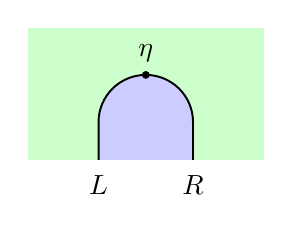
\begin{tikzpicture}[x=0.6cm,y=0.6cm, baseline=(current bounding box.center)]
        \begin{scope}       
            \clip (-2.5,0.2) rectangle (2.5,3);     
            \fill[fill=green!20] (-2.5,0.2) rectangle (2.5,3);  
            \draw[fill=blue!20, rounded corners=0.6cm, line width=0.7pt] (-1,-1) rectangle (1, 2); 
        \end{scope}
        \node[below=2pt] at (-1,0.2) {$L$};
        \node[below=2pt] at (1,0.2) {$R$};
        \node[above=1pt] at (0,2) {$\eta$};
        \draw[fill=black] (0, 2) circle (0.07);
    \end{tikzpicture}
\end{center}
defined by $\eta_X:=\Phi_{X,L(X)}\left(\mathrm{id}_{L(X)}\right)$ for any $X\in \mathrm{Ob}(\mathsf{C})$, where $\Phi_{X,L(X)}$ is the natural bijection
$$
\begin{aligned}
    \Phi_{X,L(X)}:\operatorname{Hom}_{\mathsf{D}}\left(L(X), L(X)\right) & \xlongrightarrow{\sim}\operatorname{Hom}_{\mathsf{C}}(X, RL(X)) \\
\operatorname{id}_{F(X)} & \longmapsto \eta_X 
\end{aligned}
$$
The \textbf{adjunction counit} $\varepsilon$ of this adjunction is a natural transformation
\begin{center}
    \begin{tikzcd}[ampersand replacement=\&]
        \mathsf{D} \arrow[r, "\scalebox{1.2}{$L\circ R$}"{name=A, above}, bend left=40] \arrow[r, "\scalebox{1.2}{$\mathrm{id}_{\mathsf{D}}$}"'{name=B, below}, bend right=40] 
        \&[+25pt] \mathsf{D}
        \arrow[Rightarrow, shorten <=3.5pt, shorten >=3.5pt, from=A.south-|B, to=B, "\varepsilon"]
    \end{tikzcd}
    \hspace{3cm}
    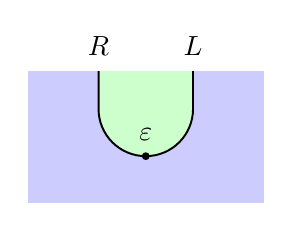
\begin{tikzpicture}[x=0.6cm,y=0.6cm, baseline=(current bounding box.center)]
        \begin{scope} 
            \clip (-2.5,0) rectangle (2.5,2.8);     
            \fill[fill=blue!20] (-2.5,0) rectangle (2.5,2.8);  
            \draw[fill=green!20, rounded corners=0.6cm, line width=0.7pt] (-1,1) rectangle (1, 4);
        \end{scope}
        \node[above=2pt] at (-1,2.8) {$R$};
        \node[above=2pt] at (1,2.8) {$L$};
        \node[above=2pt] at (0,1) {$\varepsilon$};
        \draw[fill=black] (0, 1) circle (0.07);  
    \end{tikzpicture}
\end{center}
defined by $\varepsilon_Y:=\Phi_{R(Y),Y}^{-1}\left(\mathrm{id}_{R(Y)}\right)$ for any $Y\in \mathrm{Ob}(\mathsf{D})$, where $\Phi_{R(Y),Y}^{-1}$ is the natural bijection
$$
\begin{aligned}
    \Phi_{R(Y),Y}^{-1}:\operatorname{Hom}_{\mathsf{D}}\left(R(Y), R(Y)\right) & \xlongrightarrow{\sim}\operatorname{Hom}_{\mathsf{C}}(LR(Y), R(Y)) \\
\mathrm{id}_{R(Y)} & \longmapsto \varepsilon_Y
\end{aligned}
$$
}
\pf{
    By naturality of $\Phi$, for any morphism $g:X_2\to X_1$ in $\mathsf{C}$, we have the following commutative diagram
    \[
    \begin{tikzcd}[ampersand replacement=\&]
        \mathrm{id}_{L(X_1)}\arrow[d,mapsto]\&[-30pt]\ni\&[-29pt]{\operatorname{Hom}_{\mathsf{D}}\left(L(X_1), L(X_1)\right) } \arrow[d, "{\Phi_{X_1,L(X_1)}}"'] \arrow[r,"{\left(L(g)\right)^*}"] \& [+12pt]{\operatorname{Hom}_{\mathsf{D}}\left(L(X_2), L(X_1)\right) } \arrow[d, "{\Phi_{X_2,L(X_1)}}"] \&[+12pt] {\operatorname{Hom}_{\mathsf{D}}\left(L(X_2), L(X_2)\right) } \arrow[d, "{\Phi_{X_2,L(X_2)}}"] \arrow[l,"{\left(L(g)\right)_*}"'] \&[-28pt]\in\&[-28pt]\mathrm{id}_{L(X_2)}\arrow[d,mapsto]\\[+20pt]
        \eta_{X_1}\&\ni\&{\operatorname{Hom}_{\mathsf{C}}(X_1, RL(X_1))} \arrow[r,"g^*"]                                                    \& {\operatorname{Hom}_{\mathsf{C}}(X_2, RL(X_1))}                                                   \& {\operatorname{Hom}_{\mathsf{C}}(X_2, RL(X_2))} \arrow[l, "\left(RL(g)\right)_*"']            \&[-30pt]\in\&[-30pt]\eta_{X_2}       
        \end{tikzcd}
        \]
        Since
        \[
        (L(g))^*\left(\mathrm{id}_{L(X_1)}\right)=L(g)=(L(g))_*\left(\mathrm{id}_{L(X_2)}\right),
        \]
        we have
        \[
        g^*(\eta_{X_1})=\Phi_{X_2,L(X_1)}(L(g))=\left(RL(g)\right)_*(\eta_{X_2}),
        \]   
    which implies the naturality square of $\eta$ commutes
\[
    \begin{tikzcd}[ampersand replacement=\&]
        X_2 \arrow[d, "{\eta_{X_2}}"'] \arrow[r, "g"] \&[+18pt]X_1\arrow[d, "{\eta_{X_1}}"]    \\[+15pt]
         RL(X_2)\arrow[r, "RL(g)"']\& RL(X_1)
    \end{tikzcd}
\] 
Similarly, we can show that for any morphism $h:Y_1\to Y_2$ in $\mathsf{D}$, the naturality square of $\varepsilon$ commutes
\[
    \begin{tikzcd}[ampersand replacement=\&]
        LR(Y_1) \arrow[d, "{\varepsilon_{Y_1}}"'] \arrow[r, "LR(h)"] \&[+18pt]LR(Y_2)\arrow[d, "{\varepsilon_{Y_2}}"]    \\[+15pt]
         Y_1\arrow[r, "h"']\& Y_2
    \end{tikzcd}
\]
}
\prop{Adjunction Isomorphism Determined by Unit or Counit}{
    Let $\left(L,R,\Phi\right)$ be an adjoint pair of functors and $\eta$ and $\varepsilon$ be the adjunction unit and counit respectively. Then 
   \begin{align*}
\Phi_{X,Y}(f) & =R(f) \circ \eta_X: X \rightarrow R(Y), \quad \forall f: L(X) \rightarrow Y , \\
\Phi_{X,Y}^{-1}(g) & =\varepsilon_Y \circ L(g): L(X) \rightarrow Y, \quad \forall g: X \rightarrow R(Y) .
   \end{align*}
}
\pf{
    For any object $X\in \mathrm{Ob}(\mathsf{C})$ and any morphism $f:L(X)\to Y$ in $\mathsf{D}$, we have the following commutative diagram
    \[
		\begin{tikzcd}[ampersand replacement=\&, row sep = 3.5em]
			\mathrm{id}_{L(X)}\arrow[d, mapsto]\&[-25pt]\in\&[-25pt]\mathrm{Hom}_{\mathsf{C}}(L(X),L(X)) \arrow[d, "{\Phi_{X,L(X)}}"']  \arrow[rr, "{f_*}"] \&[-15pt] \& {\mathrm{Hom}_{\mathsf{C}}(L(X),Y)}\arrow[d, "\Phi_{X,Y}"]\&[-25pt]\ni\&[-25pt]f \arrow[d, mapsto]\\
			\eta_X\&\in\&{\mathrm{Hom}_{\mathsf{C}}(X,RL(X))} \arrow[rr, "{\left(R(f)\right)_*}"'] \&  \& {\mathrm{Hom}_{\mathsf{C}}(X,R(Y))}  \&\ni\& \Phi_{X,Y}(f)     
		\end{tikzcd}
	\]
    For any object $Y\in \mathrm{Ob}(\mathsf{D})$ and any morphism $g:X\to R(Y)$ in $\mathsf{C}$, we have the following commutative diagram
    \[
        \begin{tikzcd}[ampersand replacement=\&, row sep = 3.5em]
            \mathrm{id}_{R(Y)}\arrow[d, mapsto]\&[-25pt]\in\&[-25pt]\mathrm{Hom}_{\mathsf{D}}(R(Y),R(Y)) \arrow[d, "{\Phi_{R(Y),Y}^{-1}}"']  \arrow[rr, "{g^*}"] \&[-15pt] \& {\mathrm{Hom}_{\mathsf{D}}(X,R(Y))}\arrow[d, "\Phi_{R(Y),Y}^{-1}"]\&[-25pt]\ni\&[-25pt]g \arrow[d, mapsto]\\
            \varepsilon_Y\&\in\&{\mathrm{Hom}_{\mathsf{C}}(LR(Y),Y)} \arrow[rr, "{\left(L(g)\right)^*}"'] \&  \& {\mathrm{Hom}_{\mathsf{C}}(L(X),Y)}  \&\ni\& \Phi_{X,Y}^{-1}(g)
        \end{tikzcd}
    \]
}
\lemm{Snake Equations}{
    Let $\left(L,R,\Phi\right)$ be an adjoint pair of functors and $\eta$ and $\varepsilon$ be the adjunction unit and counit respectively. Then we have the following equalities of natural transformations
    \begin{center}
        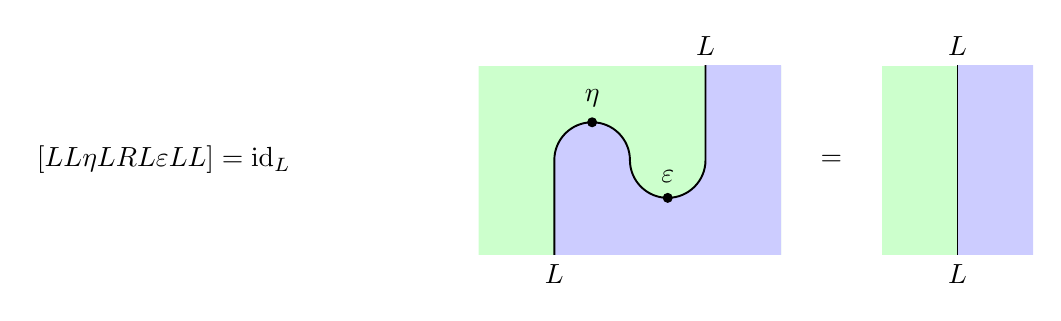
\begin{tikzpicture}[x=0.8cm,y=0.8cm]
            \node at (-7.4,1.5) {${\left[L \xRightarrow{L \eta}LR L\xRightarrow{\varepsilon L} L\right]=\mathrm{id}_L}$};
            \begin{scope} 
                \clip (-2.4,0) rectangle (2.4,3);     
                \fill[fill=green!20] (-2.5,0) rectangle (2.5,3);  
                \filldraw[fill=blue!20, rounded corners=0.48cm, line width=0.7pt] (-1.2,-1) -- (-1.2, 2.1)-- (0,2.1)-- (0,0.9)-- (1.2,0.9)
                   -- (1.2,4)-- (4,4)-- (4,-1)--cycle;
            \end{scope}
        
            \node[above] at (1.2,3) {$L$};
            \node[below] at (-1.2,0) {$L$};
        
            \draw[fill=black] (0.6, 0.9) circle (0.07);  
            \node[above=2pt] at (0.6, 0.9) {$\varepsilon$};
            
            \draw[fill=black] (-0.6, 2.1) circle (0.07); 
            \node[above=2pt] at (-0.6, 2.1) {$\eta$};
        
            \node at (3.2, 1.5) {$=$};
        
            \begin{scope} 
                \clip (4,0) rectangle (6.4,3); 
                \fill[fill=green!20] (4,0) rectangle (6.4,3); 
                \filldraw[fill=blue!20, line width=0.7pt] (5.2,-1) rectangle (7,4);  
            \end{scope} 
            
            \node[below] at (5.2,0) {$L$};
            \node[above] at (5.2,3) {$L$};
        \end{tikzpicture}
    \end{center}
    \begin{center}
        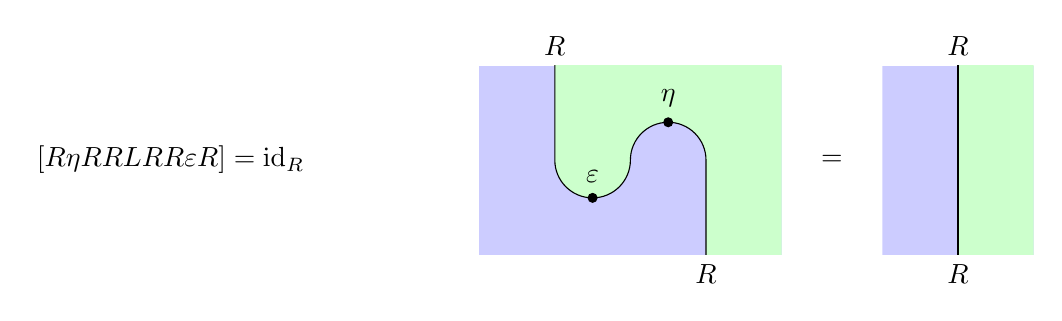
\begin{tikzpicture}[x=0.8cm,y=0.8cm]
            \node at (-7.3,1.5) {${\left[R \xRightarrow{\eta R}RLR \xRightarrow{R \varepsilon}R\right]=\mathrm{id}_R}$};
            \begin{scope} 
                \clip (-2.4, 0) rectangle (2.4, 3);     
                \fill[fill=blue!20] (-2.5, 0) rectangle (2.5,3);  
                \filldraw[fill=green!20, rounded corners=0.48cm] (-1.2, 4) -- (-1.2, 0.9)-- (0, 0.9)-- (0, 2.1)-- (1.2, 2.1)
                -- (1.2, -1)-- (4, -1)-- (4, 4)--cycle;
            \end{scope}
        
            \node[below] at (1.2,0) {$R$};
            \node[above] at (-1.2,3) {$R$};
        
            \draw[fill=black] (0.6, 2.1) circle (0.07);  
            \node[above=2pt] at (0.6, 2.1) {$\eta$};
            
            \draw[fill=black] (-0.6, 0.9) circle (0.07); 
            \node[above=2pt] at (-0.6, 0.9) {$\varepsilon$};
        
            \node at (3.2, 1.5) {$=$};
        
            \begin{scope} 
                \clip (4,0) rectangle (6.4,3); 
                \fill[fill=blue!20] (4,0) rectangle (6.4,3); 
                \filldraw[fill=green!20] (5.2,-1) rectangle (7,4);  
            \end{scope} 
            
            \node[below] at (5.2,0) {$R$};
            \node[above] at (5.2,3) {$R$};
        \end{tikzpicture}
    \end{center}
}
\dfn{Wire Bending}{
Let $\mathsf{C}$, $\mathsf{D}$, $\mathsf{C'}$, $\mathsf{D'}$ be categories and $L,R,L',R',H,K$ be functors shown in the following diagram
\[
    \begin{tikzcd}[ampersand replacement=\&]
        \mathsf{C} \arrow[dd, "L"', bend right=38] \arrow[r, "H"]  \&[+36pt] \mathsf{C'} \arrow[dd, "L'"', bend right=38] \\[-5pt]
        \dashv                                                  \& \dashv                                    \\[-5pt]
        \mathsf{D} \arrow[uu, "R"', bend right=38] \arrow[r, "K"'] \& \mathsf{D'} \arrow[uu, "R'"', bend right=38]
        \end{tikzcd}    
\]
There are bijections between the following sets of natural transformations
\[
    \begin{tikzcd}[ampersand replacement=\&]
        {\mathrm{Hom}_{[\mathsf{C}, \mathsf{D'}]}\left(L'H, KL\right) } \arrow[r, shift left=1pt, rightharpoonup, "\triangleright"]\arrow[r, shift right=1pt,leftharpoondown, "\triangleleft"']  \& {\mathrm{Hom}_{[\mathsf{C}, \mathsf{C'}]}(H, R'KL) } \arrow[d, shift left=1pt, rightharpoonup, "\triangleright"]\arrow[d, shift right=1pt,leftharpoondown, "\triangleleft"']   \\[+15pt]
        { \mathrm{Hom}_{[\mathsf{D}, \mathsf{D'}]}\left(L'HR, K\right)} \arrow[u, shift left=1pt, rightharpoonup, "\triangleright"]\arrow[u, shift right=1pt,leftharpoondown, "\triangleleft"'] \& {\mathrm{Hom}_{[\mathsf{D}, \mathsf{C'}]}(HR, R'K) } \arrow[l, shift left=1pt, rightharpoonup, "\triangleright"]\arrow[l, shift right=1pt,leftharpoondown, "\triangleleft"'] 
        \end{tikzcd}    
\]
natural in both $H$ and $K$ such that $\triangleleft=\triangleright^{-1}$ and $\triangleright\triangleright\triangleright\hspace{2.15pt}\triangleright=\triangleright^4=\mathrm{id}$. $\triangleright$ is called \textbf{wire bending} because its action can be visualized as bending the wires of adjoint pairs in the following string diagrams

\begin{center}
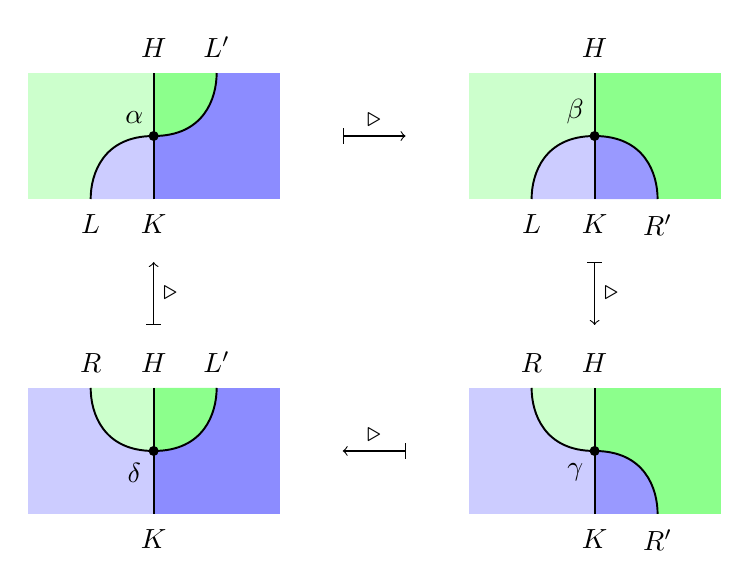
\begin{tikzpicture}[x=0.8cm,y=0.8cm, baseline=(current bounding box.center)]
    \draw [|-To] (3,1) -- (4,1) node[midway,above] {$\triangleright$};
    \draw [|-To] (7,-1) -- (7,-2) node[midway,right] {$\triangleright$};
    \draw [|-To] (4,-4) -- (3,-4) node[midway,above] {$\triangleright$};
    \draw [|-To] (0,-2) -- (0,-1) node[midway,right] {$\triangleright$};
    \begin{scope}      
        \fill[fill=green!20] (-2,0) rectangle (0,2);  
        \fill[fill=blue!45] (0,0) rectangle (2,2); 
        \fill[fill=blue!20] (-1,0) .. controls (-1,0.4) and (-0.8, 1) .. (0,1)--(0,0)--cycle;
        \fill[fill=green!45] (1,2) .. controls (1,1.6) and (0.8, 1) .. (0,1)--(0,2)--cycle;
    \end{scope}
    \draw[line width=0.7pt] (0,0) -- (0,2);
    \draw[line width=0.7pt] (-1,0) .. controls (-1, 0.4) and (-0.8, 1) .. (0, 1) .. controls (0.8, 1) and (1, 1.6) .. (1, 2);
    
    \node[above=2pt] at (0, 2) {$H$};
    \node[below=2pt] at (0, 0) {$K$};
    \node[below=2pt] at (-1, 0) {$L$};
    \node[above=2pt] at (1, 2) {$L'$};

    \draw[fill=black] (0, 1) circle (0.07);  
    \node[left=7pt, above=1pt] at (0, 1)  {$\alpha$};

\begin{scope}[shift={(7,0)}]
     \begin{scope}     
        \fill[fill=green!20] (-2,0) rectangle (0,2);  
        \fill[fill=green!45] (0,0) rectangle (2,2); 
        \fill[fill=blue!20] (-1,0) .. controls (-1, 0.4) and (-0.8, 1) .. (0,1)--(0,0)--cycle;
        \fill[fill=blue!40] (1,0) .. controls (1, 0.4) and (0.8, 1) .. (0,1)--(0,0)--cycle;
    \end{scope}
    \draw[line width=0.7pt] (0,0) -- (0,2);
    \draw[line width=0.7pt] (-1,0) .. controls (-1, 0.4) and (-0.8, 1) .. (0, 1) .. controls (0.8, 1) and (1, 0.4) .. (1, 0);
    
    \node[above=2pt] at (0, 2) {$H$};
    \node[below=2pt] at (0, 0) {$K$};
    \node[below=2pt] at (-1, 0) {$L$};
    \node[below=2pt] at (1, 0) {$R'$};

    \draw[fill=black] (0, 1) circle (0.07);  
    \node[left=7pt, above=1pt] at (0, 1)  {$\beta$};
\end{scope}
\begin{scope}[shift={(0,-5)}]
     \begin{scope}     
        \fill[fill=blue!20] (-2,0) rectangle (0,2);  
        \fill[fill=blue!45] (0,0) rectangle (2,2); 
        \fill[fill=green!20] (-1,2) .. controls (-1, 1.6) and (-0.8, 1) .. (0,1)--(0,2)--cycle;
        \fill[fill=green!45] (1,2) .. controls (1, 1.6) and (0.8, 1) .. (0,1)--(0,2)--cycle;
    \end{scope}
    \draw[line width=0.7pt] (0,0) -- (0,2);
    \draw[line width=0.7pt] (-1,2) .. controls (-1, 1.6) and (-0.8, 1) .. (0, 1) .. controls (0.8, 1) and (1, 1.6) .. (1, 2);
    
    \node[above=2pt] at (0, 2) {$H$};
    \node[below=2pt] at (0, 0) {$K$};
    \node[above=2pt] at (-1, 2) {$R$};
    \node[above=2pt] at (1, 2) {$L'$};

    \draw[fill=black] (0, 1) circle (0.07);  
    \node[left=7pt, below=1pt] at (0, 1)  {$\delta$};
\end{scope}
\begin{scope}[shift={(7,-5)}]
     \begin{scope}     
        \fill[fill=blue!20] (-2,0) rectangle (0,2);  
        \fill[fill=green!45] (0,0) rectangle (2,2); 
        \fill[fill=green!20] (-1,2) .. controls (-1, 1.6) and (-0.8, 1) .. (0,1)--(0,2)--cycle;
        \fill[fill=blue!40] (1,0) .. controls (1, 0.4) and (0.8, 1) .. (0,1)--(0,0)--cycle;
    \end{scope}
    \draw[line width=0.7pt] (0,0) -- (0,2);
    \draw[line width=0.7pt] (-1,2) .. controls (-1, 1.6) and (-0.8, 1) .. (0, 1) .. controls (0.8, 1) and (1, 0.4) .. (1, 0);
    
    \node[above=2pt] at (0, 2) {$H$};
    \node[below=2pt] at (0, 0) {$K$};
    \node[above=2pt] at (-1, 2) {$R$};
    \node[below=2pt] at (1, 0) {$R'$};

    \draw[fill=black] (0, 1) circle (0.07);  
    \node[left=7pt, below=1pt] at (0, 1)  {$\gamma$};
\end{scope}
\end{tikzpicture}
\end{center}
}
We only explicit define $\alpha^\triangleright$ here. The other wire bendings are defined similarly using the unit or counit of the adjunctions.
\begin{center} 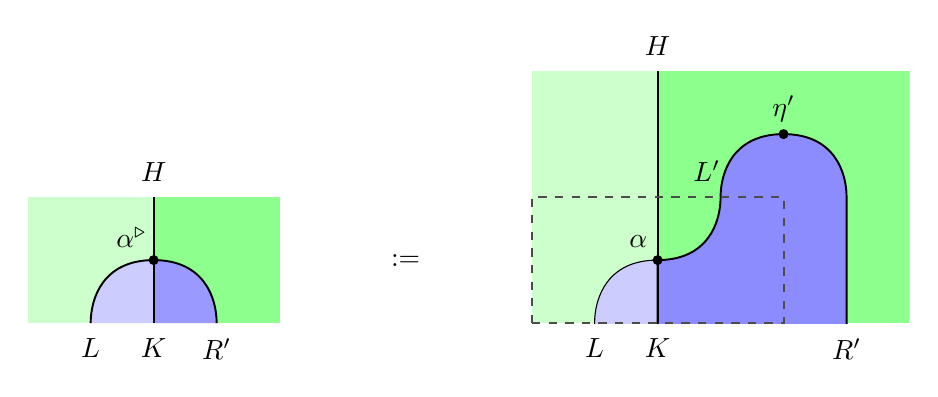
\begin{tikzpicture}[x=0.8cm,y=0.8cm, baseline=(current bounding box.center)]
    \begin{scope}     
        \fill[fill=green!20] (-2,0) rectangle (0,2);  
        \fill[fill=green!45] (0,0) rectangle (2,2); 
        \fill[fill=blue!20] (-1,0) .. controls (-1, 0.4) and (-0.8, 1) .. (0,1)--(0,0)--cycle;
        \fill[fill=blue!40] (1,0) .. controls (1, 0.4) and (0.8, 1) .. (0,1)--(0,0)--cycle;
    
    \draw[line width=0.7pt] (0,0) -- (0,2);
    \draw[line width=0.7pt] (-1,0) .. controls (-1, 0.4) and (-0.8, 1) .. (0, 1) .. controls (0.8, 1) and (1, 0.4) .. (1, 0);
    
    \node[above=2pt] at (0, 2) {$H$};
    \node[below=2pt] at (0, 0) {$K$};
    \node[below=2pt] at (-1, 0) {$L$};
    \node[below=2pt] at (1, 0) {$R'$};

    \draw[fill=black] (0, 1) circle (0.07);  
    \node[left=8pt, above=1pt] at (0, 1)  {$\alpha^{\triangleright}$};
    \end{scope}
    
    \node at (4, 1) {$:=$};
    
    \begin{scope} [shift={(8,0)}]
    \begin{scope} 
            \clip (-2,0) rectangle (4,4);     
            \fill[fill=green!20] (-2,0) rectangle (0,4);  
            \fill[fill=green!45] (0,0) rectangle (4,4);  
            \filldraw[fill=blue!20] (-1,-1) -- (-1,0) .. controls (-1,0.4) and (-0.8, 1) .. (0,1)--(0,-1)--cycle;
            \filldraw[fill=blue!45, line width=0.7pt] (0, -1) -- 
            (0, 1) .. controls (0.8, 1) and (1, 1.6) ..  
            (1, 2) .. controls (1, 2.4) and (1.2, 3) .. 
            (2, 3) .. controls (2.8, 3) and (3, 2.4) .. 
            (3, 2)--(3, -1)--cycle;
    \end{scope}
        \draw[line width=0.7pt] (0,0) -- (0,4);

        \node[above=2pt] at (0, 4) {$H$};
        \node[below=2pt] at (0, 0) {$K$};
        \node[below=2pt] at (-1, 0) {$L$};
        \node[left=5pt,above=2pt] at (1, 2) {$L'$};
        \node[below=2pt] at (3, 0) {$R'$};
    
        \draw[fill=black] (0, 1) circle (0.07);  
        \node[left=7pt, above=1pt] at (0, 1)  {$\alpha$};

        \draw[fill=black] (2, 3) circle (0.07);  
        \node[above=1pt] at (2, 3)  {$\eta'$};

        \draw[dashed, color=black!70, line width=0.7pt] (-2,0) rectangle (2,2);
    \end{scope}
    \end{tikzpicture}    
\end{center}
The fact that $\triangleleft$ is the inverse of $\triangleright$ follows from the snake equations.


\prop{Equivalent Definition of Adjoint Functor Using Unit and Counit}{
    Given pair of functors $\begin{tikzcd}[ampersand replacement=\&]
        \mathsf{C} \arrow[r, "L", bend left] \& \mathsf{D} \arrow[l, "R", bend left]
        \end{tikzcd}$
    there is a bijection between the following sets 
    \begin{align*}
        T:\left\{\text{adjoint pair }\left(L,R,\Phi\right)\right\}&\xrightleftharpoons{\;\sim\;}\left\{\left(L,R,\eta,\varepsilon\right)\text{ that satisfies snake equations}\right\}\\
        \Phi&\longmapsto\left(\eta_X:=\Phi\left(\mathrm{id}_{L(X)}\right), \varepsilon_Y:=\Phi^{-1}\left(\mathrm{id}_{R(Y)}\right)\right)\\
        \Phi_{X,Y}(f):=R(f) \circ \eta_X&\longmapsfrom(\eta, \varepsilon)
    \end{align*}
}
\pf{
    Suppose $\left(L,R,\eta,\varepsilon\right)$ satisfies snake equations. Consider the diagram
    \[
        \begin{tikzcd}[ampersand replacement=\&]
            \mathsf{1} \arrow[dd, "\mathrm{id}"', bend right=38] \arrow[r, "\diagfunctor X"]  \&[+36pt] \mathsf{C} \arrow[dd, "L"', bend right=38] \\[-5pt]
            \dashv                                                  \& \dashv                                    \\[-5pt]
            \mathsf{1} \arrow[uu, "\mathrm{id}"', bend right=38] \arrow[r, "\diagfunctor Y"'] \& \mathsf{D} \arrow[uu, "R"', bend right=38]
            \end{tikzcd}    
    \]

    \begin{center}
        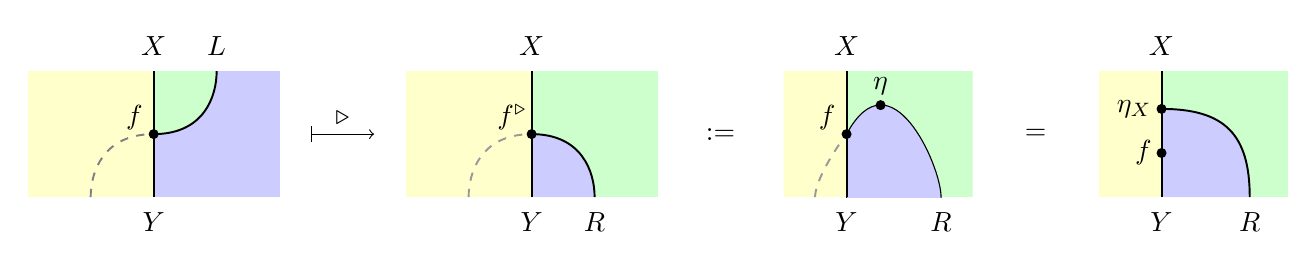
\begin{tikzpicture}[x=0.8cm,y=0.8cm, baseline=(current bounding box.center)]
        \definecolor{leftcolor}{RGB}{255,255,204}
            \draw [|-To] (2.5,1) -- (3.5,1) node[midway,above] {$\triangleright$};
            \node at (9, 1) {$:=$};
            \node at (14, 1) {$=$};
          
            \begin{scope}     
                \fill[fill=leftcolor] (-2,0) rectangle (0,2);  
                \fill[fill=blue!20] (0,0) rectangle (2,2); 
                \fill[fill=green!20] (1,2) .. controls (1,1.6) and (0.8, 1) .. (0,1)--(0,2)--cycle;
            \end{scope}
            \draw[line width=0.7pt] (0,0) -- (0,2);
            \draw[dashed, color=black!50, line width=0.7pt] (-1,0) .. controls (-1, 0.4) and (-0.8, 1) .. (0, 1) ;
            \draw[line width=0.7pt]  (0, 1) .. controls (0.8, 1) and (1, 1.6) .. (1, 2);
            
            \node[above=2pt] at (0, 2) {$X$};
            \node[below=2pt] at (0, 0) {$Y$};
            \node[above=2pt] at (1, 2) {$L$};
        
            \draw[fill=black] (0, 1) circle (0.07);  
            \node[left=7pt, above=-2pt] at (0, 1)  {$f$};
        
        \begin{scope}[shift={(6,0)}]
             \begin{scope} 
                    
                \fill[fill=leftcolor] (-2,0) rectangle (0,2);  
                \fill[fill=green!20] (0,0) rectangle (2,2); 
              
                \fill[fill=blue!20] (1,0) .. controls (1, 0.4) and (0.8, 1) .. (0,1)--(0,0)--cycle;
            \end{scope}
            \draw[line width=0.7pt] (0,0) -- (0,2);
            \draw[dashed, color=black!40, line width=0.7pt] (-1,0) .. controls (-1, 0.4) and (-0.8, 1) .. (0, 1);
            \draw[line width=0.7pt] (0, 1) .. controls (0.8, 1) and (1, 0.4) .. (1, 0);
            \node[above=2pt] at (0, 2) {$X$};
            \node[below=2pt] at (0, 0) {$Y$};
            \node[below=2pt] at (1, 0) {$R$};
        
            \draw[fill=black] (0, 1) circle (0.07);  
            \node[left=7pt, above=-2pt] at (0, 1)  {$f^{\hspace{0.2pt}\triangleright}$};
        \end{scope}
      \begin{scope}[shift={(11,0)}]
             \begin{scope} 
                \clip (-1,0) rectangle (2,2);     
                \fill[fill=leftcolor] (-2,0) rectangle (0,2);  
                \fill[fill=green!20] (0,0) rectangle (2,2); 
                \filldraw[fill=blue!20] (1.5,-1)--(1.5,0) .. controls (1.5, 0.5) and (0.7, 2.3) .. (0,1)--(0,-1)--cycle;
            \end{scope}
            \draw[line width=0.7pt] (0,0) -- (0,2);
            \draw[dashed, color=black!40, line width=0.7pt] (-0.5,0) .. controls (-0.5, 0.2) and (-0.3, 0.6) .. (0, 1);
            \node[above=2pt] at (0, 2) {$X$};
            \node[below=2pt] at (0, 0) {$Y$};
            \node[below=2pt] at (1.5, 0) {$R$};
        
            \draw[fill=black] (0, 1) circle (0.07);  
            \draw[fill=black] (0.54, 1.46) circle (0.07) node[above=0pt] {$\eta$}; 
            \node[left=7pt, above=-2pt] at (0, 1)  {$f$};
        \end{scope}

        \begin{scope}[shift={(16,0)}]
             \begin{scope}     
                \fill[fill=leftcolor] (-1,0) rectangle (0,2);  
                \fill[fill=green!20] (0,0) rectangle (2,2); 
         
                \fill[fill=blue!20] (1.4,0) .. controls (1.4,1) and (1, 1.4) .. (0,1.4)--(0,0)--cycle;
            \end{scope}
            \draw[line width=0.7pt] (0,0) -- (0,2);
         
            \draw[line width=0.7pt] (0, 1.4) .. controls (1, 1.4) and (1.4, 1) .. (1.4, 0);
            \node[above=2pt] at (0, 2) {$X$};
            \node[below=2pt] at (0, 0) {$Y$};
            \node[below=2pt] at (1.4, 0) {$R$};
        
            \draw[fill=black] (0, 0.7) circle (0.07) node[left=0pt] {$f$};  
            \draw[fill=black] (0, 1.4) circle (0.07) node[left=0pt] {$\eta_X$};  
        \end{scope}
        
        \end{tikzpicture}
    \end{center}
    As the string diagram shows, we find $\Phi_{X,Y}$ conincides with the wire bending map
    \[
        \triangleright: \mathrm{Hom}_{\mathsf{D}}\left(L(X), Y\right)\xlongrightarrow{\sim} \mathrm{Hom}_{\mathsf{C}}(X, R(Y)) 
    \]
    which is natural in both $X$ and $Y$. Hence $\Phi$ is a natural isomorphism. It is straightforward to check that $T$ is a bijection.
}

\prop{Uniqueness of Adjunction}{
    If $\left(L,R,\eta,\varepsilon\right)$ and $\left(L,R',\eta', \varepsilon\right)$ are two adjoint pairs of functors, then there is a unique natural isomorphism $\psi:R\xRightarrow{\sim} R'$ such that 
    \[
        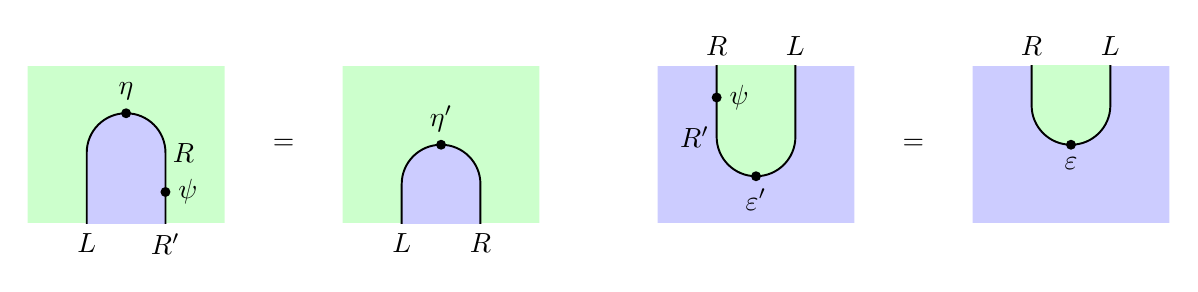
\begin{tikzpicture}[x=0.5cm,y=0.5cm,line width=0.7pt,hollow/.style={
                   circle,
                   fill=white,
                   draw,
                   outer sep=0pt,
                   inner sep=1.7pt,
                   line width=0.7pt
                 }]
           \definecolor{leftcolor}{RGB}{204, 255, 204}
           \definecolor{midcolor}{RGB}{204, 204, 255}
           
       
           \node at (4, 2) {$=$};
          \node at (20, 2) {$=$};
           
           
            \begin{scope}
               \begin{scope} 
                   \clip (-2.5,0) rectangle (2.5, 4);     
                   \fill[fill=leftcolor] (-3,0) rectangle (3, 4);  
                    
                   \draw[fill=midcolor, rounded corners=0.5cm, line width=0.7pt] (-1, -2) rectangle (1, 2.8);
               \end{scope}
             
               \filldraw [black] (1,0.8) circle (0.1) node[right=1pt] {$\psi$};
               \node[below] at (-1, 0) {$L$};
               \node[right=-1pt] at (1, 1.8) {$R$};
               \node[below] at (1, 0) {$R'$};
               \draw[fill=black] (0, 2.8) circle (0.1);
               \node[above=1pt] at (0, 2.8) {$\eta$}; 
             
           \end{scope}
           
           \begin{scope}[shift={(8,0)}]
               \begin{scope} 
                   \clip (-2.5,0) rectangle (2.5, 4); 
                   \fill[fill=leftcolor] (-3,0) rectangle (3, 4);  
                   \draw[fill=midcolor, rounded corners=0.5cm, line width=0.7pt] (-1, -2) rectangle (1, 2);
               \end{scope}
               \node[below] at (-1, 0) {$L$};
               \node[below] at (1, 0) {$R$};
               \draw[fill=black] (0, 2) circle (0.1);
               \node[above=1pt] at (0, 2) {$\eta'$}; 
           
           \end{scope}
           
           \begin{scope}[shift={(16,0)}]
               \begin{scope} 
                   \clip (-2.5,0) rectangle (2.5, 4);     
                   \fill[fill=midcolor] (-3,0) rectangle (3, 4);  
                    
                   \draw[fill=leftcolor, rounded corners=0.5cm, line width=0.7pt] (-1, 6) rectangle (1, 1.2);
               \end{scope}
             
               \filldraw [black] (-1,3.2) circle (0.1) node[right=1pt] {$\psi$};
               \node[above] at (-1, 4) {$R$};
               \node[left=-1pt] at (-1, 2.2) {$R'$};
               \node[above] at (1, 4) {$L$};
               \draw[fill=black] (0, 1.2) circle (0.1);
               \node[below=1pt] at (0, 1.2) {$\varepsilon'$}; 
             
           \end{scope}
           
           \begin{scope}[shift={(24,0)}]
               \begin{scope} 
                   \clip (-2.5,0) rectangle (2.5, 4); 
                   \fill[fill=midcolor] (-3,0) rectangle (3, 4);  
                   \draw[fill=leftcolor, rounded corners=0.5cm, line width=0.7pt] (-1, 6) rectangle (1, 2);
               \end{scope}
               \node[above] at (1, 4) {$L$};
               \node[above] at (-1, 4) {$R$};
               \draw[fill=black] (0, 2) circle (0.1);
               \node[below=1pt] at (0, 2) {$\varepsilon$}; 
           
           \end{scope}
           
        \end{tikzpicture}
    \]
}
\pf{
    Consider the diagram
    \[
        \begin{tikzcd}[ampersand replacement=\&]
            \mathsf{C} \arrow[dd, "L"', bend right=38] \arrow[r, "\mathrm{id}_{\mathsf{C}}"]  \&[+36pt] \mathsf{C} \arrow[dd, "L"', bend right=38] \\[-5pt]
            \dashv                                                  \& \dashv                                    \\[-5pt]
            \mathsf{D} \arrow[uu, "R"', bend right=38] \arrow[r, "\mathrm{id}_{\mathsf{D}}"'] \& \mathsf{D} \arrow[uu, "R'"', bend right=38]
            \end{tikzcd}    
    \]
    Define $\psi:=\mathrm{id}_L^{\:\triangleright\triangleright}$, which is illustrated by the following string diagram
    \begin{center}
        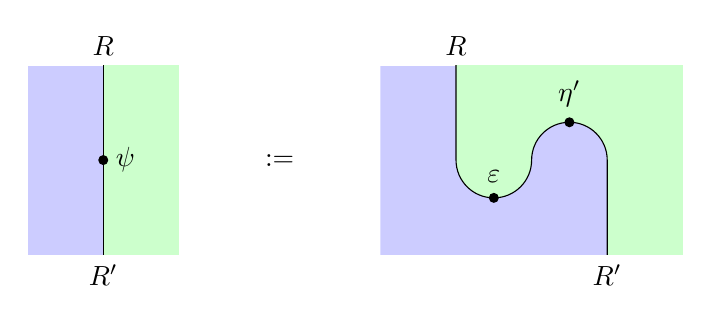
\begin{tikzpicture}[x=0.8cm,y=0.8cm]
            \node at (8, 1.5) {$:=$};
            \begin{scope}
                \begin{scope} 
                    \clip (4,0) rectangle (6.4,3); 
                    \fill[fill=blue!20] (4,0) rectangle (6.4,3); 
                    \filldraw[fill=green!20] (5.2,-1) rectangle (7,4);  
                \end{scope} 
                \draw[fill=black] (5.2, 1.5) circle (0.07) node[right=1pt] {$\psi$};
                \node[below] at (5.2,0) {$R'$};
                \node[above] at (5.2,3) {$R$};
            \end{scope}
            \begin{scope}[shift={(12,0)}] 
                \begin{scope}
                    \clip (-2.4, 0) rectangle (2.4, 3);     
                    \fill[fill=blue!20] (-2.5, 0) rectangle (2.5,3);  
                    \filldraw[fill=green!20, rounded corners=0.48cm] (-1.2, 4) -- (-1.2, 0.9)-- (0, 0.9)-- (0, 2.1)-- (1.2, 2.1)
                    -- (1.2, -1)-- (4, -1)-- (4, 4)--cycle;
                \end{scope}
        
                \node[below] at (1.2,0) {$R'$};
                \node[above] at (-1.2,3) {$R$};
            
                \draw[fill=black] (0.6, 2.1) circle (0.07);  
                \node[above=2pt] at (0.6, 2.1) {$\eta'$};
                
                \draw[fill=black] (-0.6, 0.9) circle (0.07); 
                \node[above=2pt] at (-0.6, 0.9) {$\varepsilon$};
              
            \end{scope}   
        \end{tikzpicture}
    \end{center}
    $\psi$ is a natural isomorphism since it has inverse $\mathrm{id}_L^{\:\triangleleft\triangleleft}$. The first equality in the statement of the proposition follows from $\psi^{\triangleleft}=\psi^{\triangleright\triangleright\triangleright}=\mathrm{id}_L^{\:\triangleright}=\eta'$. The uniqueness of $\psi$ follows from the injectivity of 
    $$
    \triangleleft:\mathrm{Hom}_{\left[\mathsf{D},\mathsf{C}\right]}\left(R,R'\right)\xlongrightarrow{\sim} \mathrm{Hom}_{\left[\mathsf{C},\mathsf{C}\right]}\left(\mathrm{id}_{\mathsf{C}},R'L\right).
    $$
    Similarly, the second equality follows from $\psi^{\triangleright}=\psi^{\triangleleft\triangleleft\triangleleft}=\mathrm{id}_L^{\:\triangleleft}=\varepsilon$. And the uniqueness of $\psi$ follows from the injectivity of
    $$
    \triangleright:\mathrm{Hom}_{\left[\mathsf{C},\mathsf{D}\right]}\left(L',L\right)\xlongrightarrow{\sim} \mathrm{Hom}_{\left[\mathsf{D},\mathsf{D}\right]}\left(LR,\mathrm{id}_{\mathsf{D}}\right).
    $$
}


\prop[adjunction_by_representability]{Equivalent Definition of Adjoint Functor Using Representable Functor}{
    \begin{enumerate}[(i)]
        \item A functor $L:\mathsf{C}\to\mathsf{D}$ has right adjoint if and only for each $Y\in \mathrm{Ob}(\mathsf{D})$, $\mathrm{Hom}_{\mathsf{D}}\left(L(-),Y\right)$ is representable. If so, the universal element of $\mathrm{Hom}_{\mathsf{D}}\left(L(-),Y\right)$ is $\left(R(Y), \varepsilon_Y\right)$.
        \item A functor $R:\mathsf{D}\to\mathsf{C}$ has left adjoint if and only for each $X\in \mathrm{Ob}(\mathsf{C})$, $\mathrm{Hom}_{\mathsf{C}}\left(X,R(-)\right)$ is representable. If so, the universal element of $\mathrm{Hom}_{\mathsf{C}}\left(X,R(-)\right)$ is $\left(L(X), \eta_X\right)$.
    \end{enumerate}
}
\pf{
    We only prove (i) here. The proof of (ii) is similar. 
    If $(L, R, \Phi)$ is an adjoint pair of functors, then for each $Y\in \mathrm{Ob}(\mathsf{D})$, we have an isomorphism 
    $$
    \Phi_{\text{-},Y}:\mathrm{Hom}_{\mathsf{D}}\left(L(-),Y\right)\xRightarrow{\sim} \mathrm{Hom}_{\mathsf{D}}\left(-,R(Y)\right).
    $$
    where $\Phi_{\text{-},Y}$ is the horizontal composition
    \[
        \begin{tikzcd}[ampersand replacement=\&]
            \mathsf{C}^{\mathrm{op}}\times\mathsf{1}\arrow[r,"{\mathrm{id}\times\diagfunctor Y}"]\&[+15pt]\mathsf{C}^{\mathrm{op}}\times\mathsf{D} \arrow[r, "\scalebox{1.2}{$\mathrm{Hom}_{\mathsf{D}}\left(L(-){,}-\right)$}"{name=A, above}, bend left] \arrow[r, "\scalebox{1.2}{$\mathrm{Hom}_{\mathsf{C}}\left(-{,}R(-)\right)$}"'{name=B, below}, bend right] \&[+60pt] \mathsf{Set}
            \arrow[Rightarrow, shorten <=5.5pt, shorten >=5.5pt, from=A.south-|B, to=B, "\Phi", "\sim\hspace{1.5pt}"']
        \end{tikzcd}
\]
    Since 
    \[
        \left(\Phi_{-,Y}^{-1}\right)_{R(Y)}\left(\mathrm{id}_{R(Y)}\right)=\Phi_{R(Y),Y}^{-1}\left(\mathrm{id}_{R(Y)}\right)=\varepsilon_Y,
    \]
    we see $\mathrm{Hom}_{\mathsf{D}}\left(L(-),Y\right)$ is representable by $\left(R(Y), \varepsilon_Y\right)$.

    Conversely, suppose for each $Y\in \mathrm{Ob}(\mathsf{D})$, $\mathrm{Hom}_{\mathsf{D}}\left(L(-),Y\right)$ is representable. Then for each $Y\in \mathrm{Ob}(\mathsf{D})$, there exist a natural isomorphism 
    $$
    \phi(Y):\mathrm{Hom}_{\mathsf{D}}\left(-,R_Y\right)\xRightarrow{\sim} \mathrm{Hom}_{\mathsf{D}}\left(L(-),Y\right)
    $$
    for some $R_Y\in \mathrm{Ob}(\mathsf{D})$. \Cref{th:representable_functor_by_universal_element} implies that $(R_Y,\phi(Y))$ is terminal in the category $\left(Y_{\mathsf{C}}\downarrow \mathrm{Hom}_{\mathsf{D}}\left(L(-),Y\right)\right)$, which corresponds to 
    $$ 
    \begin{tikzcd}[ampersand replacement=\&]
        \mathsf{C} \arrow[r, " Y_{\mathsf{C}}"] \& \left[\mathsf{C}^{\mathrm{op}},\mathsf{Set}\right] \&[+45pt]  \mathsf{1} \arrow[l, "{\diagfunctor \mathrm{Hom}_{\mathsf{D}}\left(L(-),Y\right)}"']
    \end{tikzcd}
    $$ 
    Given any morphism $h:Y_1\to Y_2$ in $\mathsf{D}$, since $(R_{Y_2},\phi(Y_2))$ is terminal in $\left(Y_{\mathsf{C}}\downarrow \mathrm{Hom}_{\mathsf{D}}\left(L(-),Y\right)\right)$, there exists a unique morphism $R_h:R_{Y_1}\to R_{Y_2}$  in $\mathsf{C}$ such that the following diagram commutes
     \[
     \begin{tikzcd}[ampersand replacement=\&]
        Y_{\mathsf{C}}\left(R_{Y_1}\right) \arrow[d, "Y_{\mathsf{C}}(R_h)"', dashed] \arrow[r, "\phi\left(Y_1\right)"] \&[+10pt] {\mathrm{Hom}_{\mathsf{D}}\left(L(-),Y_1\right)} \arrow[d, "h_\star"] \\[+15pt]
        Y_{\mathsf{C}}\left(R_{Y_2}\right) \arrow[r, "\phi\left({Y_2}\right)"']                                                   \& {\mathrm{Hom}_{\mathsf{D}}\left(L(-),Y_2\right)}                 
    \end{tikzcd}\hspace{3em}=\hspace{3em}
    \begin{tikzcd}[ampersand replacement=\&]
        \mathrm{Hom}_{\mathsf{C}}\left(-,R_{Y_1}\right)\arrow[d, "\left(R_h\right)_\star"', dashed] \arrow[r, "\phi\left(Y_1\right)"] \&[+10pt] {\mathrm{Hom}_{\mathsf{D}}\left(L(-),Y_1\right)} \arrow[d, "h_\star"] \\[+15pt]
        \mathrm{Hom}_{\mathsf{C}}\left(-,R_{Y_2}\right) \arrow[r, "\phi\left({Y_2}\right)"']                                                   \& {\mathrm{Hom}_{\mathsf{D}}\left(L(-),Y_2\right)}                 
    \end{tikzcd}
    \]
    Thus we can define a functor $R:\mathsf{D}\to\mathsf{C}$ by $R(Y):=R_Y$ and $R(h):= R_h$. We can also define a natural isomorphism $\Phi: \mathrm{Hom}_{\mathsf{D}}\left(L(-),-\right)\xRightarrow{\sim} \mathrm{Hom}_{\mathsf{D}}\left(-,R(-)\right)$ by
    \begin{align*}
        \Phi_{X,Y}:\mathrm{Hom}_{\mathsf{D}}\left(L(X),Y\right)&\xlongrightarrow{\sim} \mathrm{Hom}_{\mathsf{C}}\left(X,R(Y)\right)\\
        \Big(L(X)\xlongrightarrow{f}Y\Big)&\longmapsto \Big(X\xlongrightarrow{\left(\phi(Y)_X\right)^{-1}(f)}R(Y)\Big)
    \end{align*}
    The naturality of $\Phi$ can be check as follows: for any morphism $g:X_2\to X_1$ in $\mathsf{C}$ and $h:Y_1\to Y_2$ in $\mathsf{D}$, the following diagram commutes
    \[
        \begin{tikzcd}[ampersand replacement=\&]
            \mathrm{Hom}_{\mathsf{D}}\left(L(X_1),Y_1\right) \arrow[r, "L(g)^*"] \arrow[d, "\Phi_{X_1,Y_1}"', "\left(\phi(Y_1)_{X_1}\right)^{-1}"] \&[+40pt]\mathrm{Hom}_{\mathsf{D}}\left(L(X_2),Y_1\right) \arrow[r, "{h_*}"]\arrow[d, "\Phi_{X_2,Y_1}"', "\left(\phi(Y_1)_{X_2}\right)^{-1}"] \&[+40pt] \mathrm{Hom}_{\mathsf{D}}\left(L(X_2),Y_2\right) \arrow[d, "\Phi_{X_2,Y_2}"', "\left(\phi(Y_2)_{X_2}\right)^{-1}"] \\[+20pt]
            \mathrm{Hom}_{\mathsf{C}}\left(X_1,R(Y_1)\right) \arrow[r, "{g^*}"'] \&\mathrm{Hom}_{\mathsf{C}}\left(X_2,R(Y_1)\right) \arrow[r, "{R(h)_*}"']\& \mathrm{Hom}_{\mathsf{C}}\left(X_2,R(Y_2)\right)
        \end{tikzcd}
    \]
    Therefore, $(L,R,\Phi)$ is an adjoint pair of functors.
}

\cor{Equivalent Definition of Adjoint Functor Using Universal Morphism}{
    Given pair of functors $\begin{tikzcd}[ampersand replacement=\&]
        \mathsf{C} \arrow[r, "L", bend left] \& \mathsf{D} \arrow[l, "R", bend left]
        \end{tikzcd}$, then the following are equivalent
    \begin{enumerate}[(i)]
        \item $L \dashv R$.
        \item For every object $X\in\mathrm{Ob}(\mathsf{C})$, there exists $\left(L(X), X\xrightarrow{\eta_X} R(L(X))\right)$ initial in $\left(X\downarrow R\right)$, i.e. there exists a \hyperref[th:universal_morphism]{universal morphism} from $X$ to $R$.
        \item For every object $Y\in\mathrm{Ob}(\mathsf{D})$, there exists $\left(R(Y), L(R(Y))\xrightarrow{\varepsilon_Y} Y\right)$ terminal in $\left(L\downarrow Y\right)$, i.e. there exists a \hyperref[th:universal_morphism]{universal morphism} from $L$ to $Y$.
    \end{enumerate} 
}
\pf{
    This is a direct consequence of \Cref{th:adjunction_by_representability}. According to \Cref{th:universal_morphism_by_representability}, for each $X\in\mathrm{Ob}(\mathsf{C})$, $\mathrm{Hom}_{\mathsf{C}}\left(X,R(-)\right)$ is representable by $\left(L(X),\eta_X\right)$ is equivalent to that $\left(L(X), X\xrightarrow{\eta_X} R(L(X))\right)$ is initial in $\left(X\downarrow R\right)$.

    \[
        \begin{tikzcd}[ampersand replacement=\&]
            X \arrow[r, "\eta_X"] \arrow[rd, "g"'] \&[+20pt] R(L(X)) \arrow[d, "R\left(g^{\triangleleft}\right)", dashed] \&[+50pt]    \{*\} \arrow[r, "\diagfunctor \eta_X"] \arrow[rd, "\diagfunctor g"'] \&[+15pt] \mathrm{Hom}_{\mathsf{C}}\left(X,R(L(X))\right) \arrow[d, "R\left(g^{\triangleleft}\right)_*", dashed] \\[+20pt]
            \& R(Y) \&\& \mathrm{Hom}_{\mathsf{C}}\left(X,R(Y)\right)     
        \end{tikzcd}
    \]

    Similarly, for each $Y\in\mathrm{Ob}(\mathsf{D})$, $\mathrm{Hom}_{\mathsf{D}}\left(L(-),Y\right)$ is representable by $\left(R(Y), \varepsilon_Y\right)$ is equivalent to that $\left(R(Y), \varepsilon_Y\right)$ is terminal in $\left(L\downarrow Y\right)$.
    \[
        \begin{tikzcd}[ampersand replacement=\&]
            L(X) \arrow[d, "L\left(f^{\triangleright}\right)"', dashed] \arrow[rd, "f"] \&[+20pt]   \&[+50pt]   {\mathrm{Hom}_{\mathsf{D}}\left(L(X),Y\right)}     \&[+15pt]  \\[+20pt]
            L(R(Y)) \arrow[r, "\eta_Y"']   \& Y \&  {\mathrm{Hom}_{\mathsf{D}}\left(L(R(Y)),Y\right)} \arrow[u, "L\left(f^{\triangleright}\right)^*", dashed] \& \{*\} \arrow[lu, "\diagfunctor f"'] \arrow[l, "\diagfunctor\eta_Y"]
        \end{tikzcd}
    \]
}

\section{Monoidal Category}
\dfn{Monoidal Category}{
    A monoidal category is a category $\mathsf{V}$ equipped with
    \begin{enumerate}[(i)]
        \item Tensor product: a functor $\otimes:\mathsf{V}\times\mathsf{V}\to\mathsf{V}$.
        \[
            \begin{tikzcd}[ampersand replacement=\&]
                \mathsf{V}\times \mathsf{V}\&[-25pt]\&[+10pt]\&[-30pt] \mathsf{V}\&[-30pt]\&[-30pt] \\ [-15pt] 
                (X_1,Y_1)  \arrow[dd, "f\times g"{name=L, left}] 
                \&[-25pt] \& [+10pt] 
                \& [-30pt]X_1\otimes Y_1\arrow[dd, "f\otimes g"{name=R}] \\ [-10pt] 
                \&  \phantom{.}\arrow[r, "\otimes", squigarrow]\&\phantom{.}  \&   \\[-10pt] 
                (X_2,Y_2)  \& \& \& X_2\otimes Y_2
            \end{tikzcd}
            \]
        \item Associator: a natural isomorphism $a$
        \[
            \begin{tikzcd}[ampersand replacement=\&]
                \mathsf{V}\times\mathsf{V}\times\mathsf{V} \arrow[r, "(-\otimes-)\otimes-"{name=A, above}, bend left] \arrow[r, "-\otimes(-\otimes-)"'{name=B, below}, bend right] \&[+30pt] \mathsf{V}
                \arrow[Rightarrow, shorten <=5.5pt, shorten >=5.5pt, from=A.south-|B, to=B, "a", "\sim\hspace{1pt}"']
            \end{tikzcd}
        \]
        \item Unit object: an object $1\in \mathrm{Ob}(\mathsf{V})$ 
        \item An isomorphism in $\mathsf{V}$: $\iota:1\otimes 1\to 1$
    \end{enumerate}
    such that the following two condition holds
    \begin{enumerate}[(i)]
        \item The pentagon axiom: the following diagram commutes
    \[
        \begin{tikzcd}[ampersand replacement=\&, column sep=small]
            \& [-50pt]                  \&[-25pt]    ((A\otimes B)\otimes C)\otimes D \arrow[lld, "{a_{(A,B,C)}\otimes \mathrm{id}_D}"'] \arrow[rrd, "{a_{(A\otimes B,C,D)}}"] \& [-25pt]                  \&   [-50pt]                                                                      \\[+20pt]
(A\otimes( B\otimes C))\otimes D \arrow[rd, "{a_{(A,B\otimes C,D)}}"'] \&                                                                                    \&    \&       \& (A\otimes B)\otimes (C\otimes D) \arrow[ld, "{a_{(A, B, C\otimes D)}}"] \\[+35pt]
            \& A\otimes( (B\otimes C)\otimes D) \arrow[rr, "{\mathrm{id}_A\otimes a_{(B,C,D)}}"'] \&    \& A\otimes( B\otimes (C\otimes D)) \&                                                                        
\end{tikzcd}
    \]
    \item Unit axiom: the functors $1\otimes -:\mathsf{V}\to\mathsf{V}$ and $-\otimes 1:\mathsf{V}\to\mathsf{V}$ are category equivalences.
    \end{enumerate}
}

A strict monoidal category is one for which the natural isomorphisms $a$, $\lambda$ and $\rho$ are identities. Every monoidal category is monoidally equivalent to a strict monoidal category.

\dfn{Cartesian/Cocartesian Monoidal Category}{
    \begin{itemize}[leftmargin=8pt]
        \item A \textbf{cartesian monoidal category} is a monoidal category with finite products endowed with a where the tensor product is the categorical product and the unit object is the terminal object. If a category has all finite products, then we say it is \textbf{cartesian monoidal}. 
        \item A \textbf{cocartesian monoidal category} is a monoidal category where the tensor product is the categorical coproduct and the unit object is the initial object. If a category has all finite coproducts, then we say it is \textbf{cocartesian monoidal}.
    \end{itemize}
}

\ex{Category of Endofunctors is a Monoidal Category}{
    Let $\mathsf{C}$ be a category. The \textbf{category of endofunctors} $\left[\mathsf{C},\mathsf{C}\right]$ is a monoidal category with the following structure
    \begin{enumerate}[(i)]
        \item Tensor product: composition of functors.
        \item Associator: the natural isomorphism $a$ is the identity.
        \item Unit object: the identity functor $\mathrm{id}_{\mathsf{C}}$.
        \item Unit isomorphism: the natural isomorphism $\iota$ is the identity.
    \end{enumerate}
}

\dfn{Braided Monoidal Category}{
    A \textbf{braided monoidal category} is a monoidal category $\mathsf{V}$ equipped with an isomorphism natural in $X,Y\in \mathrm{Ob}(\mathsf{V})$
    \[
        B_{X,Y} : X \otimes Y \to Y \otimes X
    \]
    called the \textbf{braiding} such that the following two conditions hold:
    \begin{enumerate}[(i)]
        \item The hexagon axiom: the following diagram commutes
        \[
            \begin{tikzcd}[ampersand replacement=\&, column sep=small]
                \&[-50pt] (X\otimes Y)\otimes Z\arrow[rr, "{B_{X\otimes Y,Z}}"]\&[+45pt]  \&[-25pt] Z\otimes (X\otimes Y) \arrow[rd, "{a_{Z,X,Y}^{-1}}"] \&[-50pt] \\[+20pt]
                X\otimes (Y\otimes Z)\arrow[ru, "{a_{X,Y,Z}^{-1}}"] \arrow[rd, "{\mathrm{id}_X\otimes B_{Y,Z}}"'] \& \& \& \& (Z\otimes X)\otimes Y \\[+35pt]
                \& X\otimes (Z\otimes Y) \arrow[rr, "{a_{X,Z,Y}^{-1}}"'] \& \& (X\otimes Z)\otimes Y\arrow[ru, "{B_{X,Z}\otimes\mathrm{id}_Y}"']  \& 
            \end{tikzcd}
        \]
    \end{enumerate}
}

\dfn{Symmetric Monoidal Category}{
    A \textbf{symmetric monoidal category} is a braided monoidal category $\mathsf{V}$ satisfying the following condition:
    \[
        B_{Y,X}\circ B_{X,Y}=\mathrm{id}_{X\otimes Y}.
    \]
}
\section{Enriched Category}
\dfn{Enriched Category}{
    Let $\mathsf{V}$ be a monoidal category. An \textbf{$\mathsf{V}$-enriched category} $\mathsf{C}$ consists of
    \begin{enumerate}[(i)]
        \item Object set: a set of objects $\mathrm{Ob}(\mathsf{C})$.
        \item $\mathrm{Hom}$-object: for each pair of objects $A,B\in \mathrm{Ob}(\mathsf{C})$, an object $\mathrm{Hom}_{\mathsf{C}}(A,B)\in \mathrm{Ob}(\mathsf{V})$.
        \item Composition: for each triple of objects $A,B,C\in \mathrm{Ob}(\mathsf{C})$, a morphism in $\mathsf{V}$
        \[
            \circ:\mathrm{Hom}_{\mathsf{C}}(B,C)\otimes \mathrm{Hom}_{\mathsf{C}}(A,B)\longrightarrow \mathrm{Hom}_{\mathsf{C}}(A,C)
        \]
        \item Identity: for each object $A\in \mathrm{Ob}(\mathsf{C})$, a morphism ${\mathcal{I}d}_A:1 \to \mathrm{Hom}_{\mathsf{C}}(A,A)$ in $\mathsf{V}$.
    \end{enumerate}
    such that the following conditions hold
    \begin{enumerate}[(i)]
        \item For each quadruple of objects $A,B,C,D\in \mathrm{Ob}(\mathsf{C})$, the following diagram in $\mathsf{V}$ commutes
        \[
            \begin{tikzcd}[ampersand replacement=\&, column sep=small]
                    \&[-130pt] {\left(\mathrm{Hom}(C,D)\otimes \mathrm{Hom}(B,C)\right)\otimes \mathrm{Hom}(A,B) } \arrow[ld, "\circ\;\otimes \,\mathrm{id}_{\mathrm{Hom}(A,B)}"'] \arrow[rr, "\cong"] \&  [-30pt]   \&  [-30pt]{\mathrm{Hom}(C,D)\otimes \left(\mathrm{Hom}(B,C)\otimes \mathrm{Hom}(A,B)\right) } \arrow[rd, "\mathrm{id}_{\mathrm{Hom}(C,D)}\,\otimes\;\circ "] \&  [-130pt]  \\[+35pt]
{\mathrm{Hom}(B,D)\otimes \mathrm{Hom}(A,B) } \arrow[rrd, "\circ"'] \&                                                                                                                                    \&                                               \&                                                                                                               \& {\mathrm{Hom}(C,D)\otimes \mathrm{Hom}(A,C) } \arrow[lld, "\circ"] \\[+20pt]
                    \&                                                                                                                                    \& {\mathrm{Hom}(A,D)} \&                                                                                                               \&                                                                   
\end{tikzcd}
    \]
    \item For each pair of objects $A,B\in \mathrm{Ob}(\mathsf{C})$, the following diagrams in $\mathsf{V}$ commute
    \[
    \begin{tikzcd}[ampersand replacement=\&, column sep=small]
        {1\otimes \mathrm{Hom}_{\mathsf{C}}(A,B)} \arrow[rr, "{{\mathcal{I}d}_B\otimes\,\mathrm{id}_{\mathrm{Hom}_{\mathsf{C}}(A,B)}}"] \arrow[rd, "\cong"'] \&                     \& {\mathrm{Hom}_{\mathsf{C}}(B,B)\otimes \mathrm{Hom}_{\mathsf{C}}(A,B)} \arrow[ld, "\circ"] \\[+10pt]
        \& {\mathrm{Hom}_{\mathsf{C}}(A,B)} \&   
\end{tikzcd}
    \]
    \[
        \begin{tikzcd}[ampersand replacement=\&, column sep=small]
            {\mathrm{Hom}_{\mathsf{C}}(A,B)\otimes 1} \arrow[rr, "\mathrm{id}_{\mathrm{Hom}_{\mathsf{C}}(A,B)}\otimes\,{\mathcal{I}d}_A "] \arrow[rd, "\cong"'] \&                     \& {\mathrm{Hom}_{\mathsf{C}}(A,B)\otimes \mathrm{Hom}_{\mathsf{C}}(A,A)} \arrow[ld, "\circ"] \\[+10pt]
            \& {\mathrm{Hom}_{\mathsf{C}}(A,B)} \&
    \end{tikzcd}
        \]
    \end{enumerate}
}

\section{2-Category}

\dfn{Strict 2-Category}{
    Let $\mathsf{Cat}$ be the Cartesian monoidal category consisting of all small categories. A \textbf{strict 2-category} is a $\mathsf{Cat}$-enriched category. We define the following sets
    \begin{itemize}
        \item 0-morphism set: $\mathrm{Ob}(\mathsf{C})$
        \item 1-morphism set: $\mathrm{Hom}_{\mathsf{C}}(X,Y)$ for any $X,Y\in \mathrm{Ob}(\mathsf{C})$
        \item 2-morphism set: $\mathrm{Hom}_{\mathsf{C}}(f,g)$ for any $X,Y\in \mathrm{Ob}(\mathsf{C})$ and $f,g\in \mathrm{Hom}_{\mathsf{C}}(X,Y)$
    \end{itemize}

    For any $X,Y,Z\in\mathrm{Ob}(\mathsf{C})$, we have the following composition bifunctor
    \begin{align*}
        \begin{tikzcd}[ampersand replacement=\&]
            \mathrm{Hom}_{\mathsf{C}}(Y,Z)\times \mathrm{Hom}_{\mathsf{C}}(X,Y)\&[-25pt]\&[+10pt]\&[-30pt] \mathrm{Hom}_{\mathsf{C}}(X,Z)\&[-30pt]\&[-30pt] \\ [-15pt] 
            (f',f)  \arrow[dd, "{(\theta', \theta)}"{name=L, left},Rightarrow] 
            \&[-25pt] \& [+10pt] 
            \& [-30pt]f'\circ f\arrow[dd, "\theta'\circ \theta"{name=R},Rightarrow] \\ [-10pt] 
            \&  \phantom{.}\arrow[r, "\Theta", squigarrow]\&\phantom{.}  \&   \\[-10pt] 
            (g',g)  \& \& \& g'\circ g
        \end{tikzcd}
    \end{align*}
    which are called the horizontal composition of 2-morphisms. The functoriality of $\Theta$ means that given any vertical composition of 2-morphisms
    \[
        \begin{tikzcd}[ampersand replacement=\&]
            { (f',f)} \arrow[d, "{(\theta', \theta)}"', Rightarrow] \\
            { (g',g)} \arrow[d, "{(\psi', \psi)}"', Rightarrow]     \\
            { (h',h)}                                              
        \end{tikzcd}
    \]
    we have the following equality
    \begin{align*}
        \Theta\left(\left(\psi'\circ\theta'\right),\left(\psi\circ\theta\right)\right)=\left(\psi'\circ\theta'\right)\circ\left(\psi\circ\theta\right)=\Theta\left(\psi',\psi\right)\circ\Theta\left(\theta',\theta\right)=\left(\psi'\circ\psi\right)\circ\left(\theta'\circ\theta\right)
    \end{align*}
    which is called the \textbf{interchange law}.
}

\ex{$\mathsf{Cat}$ as 2-category}{
    The category $\mathsf{Cat}$ is a strict 2-category with the following structure
    \begin{itemize}
        \item 0-morphism set: $\mathrm{Ob}(\mathsf{Cat})$
        \item 1-morphism set: $\mathrm{Hom}_{\mathsf{Cat}}(\mathsf{C},\mathsf{D}):=[\mathsf{C},\mathsf{D}]$ for any $\mathsf{C},\mathsf{D}\in \mathrm{Ob}(\mathsf{Cat})$
        \item 2-morphism set: $\mathrm{Hom}_{\mathsf{Cat}}(F,G):=\mathrm{Hom}_{[\mathsf{C},\mathsf{D}]}\left(F,G\right)$ for any $\mathsf{C},\mathsf{D}\in \mathrm{Ob}(\mathsf{Cat})$ and $F,G\in [\mathsf{C},\mathsf{D}]$
    \end{itemize}
}
\section{Internalization}
Traditional Bourbaki-style mathematical structures are formulated within set theory, or put differently, within the ambient category $\mathsf{Set}$. The concept of \textbf{Internalization} entails reformulating these mathematical structures in a broader ambient category $\mathsf{C}$, which typically need some extra structures to express the correponding mathematics. The extra structure required on an ambient category $\mathsf{C}$ is referred to as a \textbf{doctrine} for internalization.

\subsection{Monoid Object}
Monoids can be internalized in the doctrine of monoidal categories.

\ex{Monoid Objects in Monoidal Categories}{
    Monoid objects internal to Cartesian monoidal categories
    \begin{itemize}
        \item $\mathsf{Set}$: traditional monoid.
        \item $\mathsf{Cat}$: (small) strict monoidal category.
        \item $\mathsf{Top}$: topological monoid.
        \item $\mathsf{Mon}$: commutative monoid.
    \end{itemize}
    Monoid objects internal to general monoidal categories
    \begin{itemize}
        \item $(R\text{-}\mathsf{Mod},\otimes_{R}, R)$ for $R\in \mathrm{Ob}(\mathsf{CRing})$: associative $R$-algebra.
        \item $(\mathsf{Ab},\otimes_{\mathbb{Z}}, \mathbb{Z})$: ring.
        \item $\left(\mathsf{Ch}\left(R\text{-}\mathsf{Mod}\right),\otimes_{R}, (R)_{n\in\mathbb{Z}}\right)$ for $R\in \mathrm{Ob}(\mathsf{CRing})$:  differential graded $R$-algebra.
        \item $\left([\mathsf{C},\mathsf{C}], \circ, \mathrm{id}_{\mathsf{C}}\right)$ for $\mathsf{C}\in \mathrm{Ob}(\mathsf{Cat})$: monad on $\mathsf{C}$.
    \end{itemize}
}
Commutative monoids can be internalized in the doctrine of symmetric monoidal categories.


\subsection{Internal Category}

\dfn{Internal Category}{
    Let $\mathsf{C}$ be a category with pullbacks. A \textbf{category internal to $\mathsf{C}$} consists of
    \begin{enumerate}[(i)]
        \item Object of 0-morphisms: an object $C_0\in \mathrm{Ob}(\mathsf{C})$.
        \item Object of 1-morphisms: an object $C_1\in \mathrm{Ob}(\mathsf{C})$.
        \item Source and target morphisms: two morphisms $s,t:C_1\to C_0$.
        \item Identity assignment: a morphism $e:C_0\to C_1$.
        \item Composition: a morphism $c:C_1\times_{C_0}C_1\to C_1$.
    \end{enumerate}
    such that the following diagrams commute
    \begin{enumerate}[(i)]
        \item Source and target of identity morphisms
        \[
            \begin{tikzcd}[ampersand replacement=\&]
                \& C_0\arrow[rd, "\mathrm{id}_{C_0}"]  \arrow[ld, "\mathrm{id}_{C_0}"']\arrow[d, "e"] \&   \\
                C_0  \& C_1  \arrow[l, "s"] \arrow[r, "t"']    \&   C_0
            \end{tikzcd}
        \]
        \item Source and target of composition
        \[
            \begin{tikzcd}[ampersand replacement=\&]
                C_1\arrow[d, "s"'] \&C_1\times_{C_0}C_1 \arrow[d, "c"]\arrow[l, "\pi_1"']\arrow[r, "\pi_2"] \& C_1 \arrow[d, "t"] \\
                C_0\&C_1 \arrow[l, "s"]\arrow[r, "t"'] \& C_0                  
            \end{tikzcd}
        \]
        \item Associativity of composition 
        \item Left and right unit laws       
    \end{enumerate}
}

\dfn{Double Category}{
    A \textbf{double category} $\mathsf{D}$ is a category internal to $\mathsf{Cat}$.
}

\section{Abelian Category}
Some literature refers to $\mathsf{Ab}$-categories as preadditive categories. We will not use this term in this note.



\dfn{Biproduct}{
    Let $\mathsf{C}$ be an $\mathsf{Ab}$-category and $X_1$, $X_2$ be objects in $\mathsf{C}$. A \textbf{biproduct} of $X_1$ and $X_2$ is a diagram
    \[
    \begin{tikzcd}[ampersand replacement=\&]
            X_1 \arrow[r, "i_1", shift left] \& X_1\oplus X_2 \arrow[l, "p_1", shift left] \arrow[r, "p_2"', shift right] \& X_2 \arrow[l, "i_2"', shift right]
    \end{tikzcd}
    \]
    such that
    \begin{itemize}
        \item $p_1\circ i_1=\mathrm{id}_{X_1}$, $p_2\circ i_2=\mathrm{id}_{X_2}$.
        \item $i_1\circ p_1+ i_2\circ p_2=\mathrm{id}_{X_1\oplus X_2}$.
    \end{itemize}
    Empty biproduct is defined to be the zero object.
}

\prop{Equivalent Conditions of Existance of Biproduct}{
    Let $\mathsf{C}$ be an $\mathsf{Ab}$-category and $X_1$, $X_2$ be objects in $\mathsf{C}$. Then the following are equivalent
    \begin{enumerate}[(i)]
        \item Product $X_1\times X_2$ exists.
        \item Coproduct $X_1\amalg X_2$ exists.
        \item Biproduct $X_1\oplus X_2$ exists.
    \end{enumerate}
}
\prop{Equivalent Conditions of Existance of Zero Object}{
    Let $\mathsf{C}$ be an $\mathsf{Ab}$-category. Then the following are equivalent
    \begin{enumerate}[(i)]
        \item Initial object (empty product) exists.
        \item Terminal object (empty coproduct) exists.
        \item Zero object (empty biproduct) exists.
    \end{enumerate}
}
\prop{$\mathsf{Ab}$-enriched functors preserve biproducts}{
    $\mathsf{Ab}$-enriched functors preserve finite biproducts.
}
\dfn{Additive Category}{
    An $\mathsf{Ab}$-category is \textbf{additive} if it has all finite biproducts.
}

\dfn{Kernel and Cokernel}{
    Suppose $\mathsf{C}$ is an abelian category with zero object and $f:X\to Y$ is a morphism in $\mathsf{C}$. The \textbf{kernel} of $f$ is the equalizer of $f$ and the zero morphism, which is denoted by $\ker f$. The universal property of kernel is given by the following diagram
    \[
    \begin{tikzcd}[ampersand replacement=\&]
        \& M \arrow[d, "g"] \arrow[rd, "0"] \arrow[ld, "\exists!\widetilde{g}"', dashed] \&   \\
        \ker f \arrow[r] \& X \arrow[r, "f"']                                                             \& Y
    \end{tikzcd}
    \]
    The \textbf{cokernel} of $f$ is the coequalizer of $f$ and the zero morphism, which is denoted by $\operatorname{coker}f$. The universal property of cokernel is given by the following diagram
    \[
    \begin{tikzcd}[ampersand replacement=\&]
        \& M                           \&                                                                     \\
        X \arrow[r, "f"'] \arrow[ru, "0"] \& Y \arrow[u, "g"'] \arrow[r] \& \operatorname{coker} f \arrow[lu, "\exists!\widetilde{g}"', dashed]
        \end{tikzcd}
    \]

}

\dfn{Abelian Category}{
    An additive category $\mathsf{C}$ is \textbf{abelian} if 
    \begin{enumerate}[(i)]
        \item Every morphism has both a kernel and a cokernel.
        \item Every monomorphism and every epimorphism is normal. This means that every monomorphism is a kernel of some morphism, and every epimorphism is a cokernel of some morphism.
    \end{enumerate}
}

\prop{}{
    If $\mathsf{A}$ is an abelian category, then $\left[\mathsf{C}^\mathrm{op}, \mathsf{A}\right]$ is abelian for any small category $\mathsf{C}$.
}
